\documentclass[11pt,a4paper]{article}

\setlength{\marginparwidth}{2cm}
\usepackage[colorinlistoftodos,prependcaption,textsize=tiny]{todonotes}

%% The xcolor package is required to highlight table rows with 
%% different colors. 
\usepackage{longtable}
\usepackage{multirow}
% Sideway figures and tables. 
\usepackage{rotating}


% ----------- Miscellaneous packages
\usepackage{enumitem}
\usepackage{chemformula}
\usepackage[version=4]{mhchem}

\usepackage[ampersand,sharp]{easylist}


% ----------- ADD COMMENT COMMANDS --------------------
\newcommand{\ruby}[1]{\todo[color=green!40]{#1 - Ruby}}
\newcommand{\studentX}[1]{\todo[color=green!40]{#1 - studentX}} % replace studentX with your name. 
\newcommand{\vicente}[1]{\todo[color=purple!40]{#1 - vicente}}
\newcommand{\david}[1]{\todo[color=yellow]{#1 - david}}
% -----------------------------------------------------
\usepackage[margin=2.5cm]{geometry}
\usepackage[T1]{fontenc}
\usepackage{lmodern}
\usepackage{amsmath,amssymb}
\usepackage[round,authoryear]{natbib}
\usepackage[hidelinks]{hyperref}
\usepackage{enumitem}
\setlist[itemize]{itemsep=2pt,topsep=4pt}
\setlist[enumerate]{itemsep=3pt,topsep=4pt}

\newcommand{\R}{\mathbb{R}}
\newcommand{\Z}{\mathbb{Z}}
\newcommand{\N}{\mathbb{N}}
\newcommand{\Q}{\mathbb{Q}}
\newcommand{\C}{\mathbb{C}}
\newcommand{\F}{{\mathbb F}}
\newcommand{\Pb}{{\mathbb P}}
\newcommand{\E}{{\mathbb E}}
\newcommand{\Frac}[2]{\left(\frac{#1}{#2}\right)}
\newcommand{\Eval}[2]{\big|_{#1}^{#2}}
\newcommand{\intinf}{\int_{-\infty}^{\infty}}

\newenvironment{theorem}[2][Theorem]{\begin{trivlist}
\item[\hskip \labelsep {\bfseries #1}\hskip \labelsep {\bfseries #2.}]}{\end{trivlist}}
\newenvironment{lemma}[2][Lemma]{\begin{trivlist}
\item[\hskip \labelsep {\bfseries #1}\hskip \labelsep {\bfseries #2.}]}{\end{trivlist}}
\newenvironment{exercise}[2][Exercise]{\begin{trivlist}
\item[\hskip \labelsep {\bfseries #1}\hskip \labelsep {\bfseries #2.}]}{\end{trivlist}}
\newenvironment{problem}[2][Problem]{\begin{trivlist}
\item[\hskip \labelsep {\bfseries #1}\hskip \labelsep {\bfseries #2.}]}{\end{trivlist}}
\newenvironment{question}[2][Question]{\begin{trivlist}
\item[\hskip \labelsep {\bfseries #1}\hskip \labelsep {\bfseries #2.}]}{\end{trivlist}}
\newenvironment{corollary}[2][Corollary]{\begin{trivlist}
\item[\hskip \labelsep {\bfseries #1}\hskip \labelsep {\bfseries #2.}]}{\end{trivlist}}

\newenvironment{solution}{\begin{proof}[Solution]}{\end{proof}}

\title{Continuous-Time Stochastic Processes\\\large Advanced Course --- Bariloche, 2026}
\author{David Alonso}
\date{}

\begin{document}
\maketitle
\tableofcontents
% % ================================================================
% Drop-in section for notes.tex
% Requires \usepackage{amsmath,amssymb} and \usepackage{natbib}.
% Bibliography entries: advanced_stochastic_processes_readings.bib
% ================================================================

\section{Basic Concepts, Definitions, and Examples}
\subsection{Random variables and Probability Distributions}

\subsubsection{Review Random Variables }
Review the definition of integer-value random variables -- conceptually, as variables that take values as the result of an experiment. 

\subsubsection{Probability Generating Functions} 
Probability generating functions are an extremely useful way to describe random variables. For an integer-valued random variable $X$ such that $\Pb[X=j] = p_j$, the probability generating function is defined as 

$$ G(x) = \sum_{j=0}^{\infty}p_j x^j. $$

Note that we can easily calculate the expected value

$$G'(1) = \sum_{n=1}^{\infty} p_n n x^{n-1} = \sum_{n=0}^{\infty} n p_n = \E[X]$$,

and similarly higher moments (variance, etc.). 

u\ruby{More explanation here. Explicit description of how the equation for variance can be found using the generating function.}

\bigskip

\textbf{Some useful facts:} \\

\begin{easylist}[itemize]
  & Example: Convolution (sums)
      && Let $X$ and $Y$ be random variables with probability generating functions $G_X(u)$ and $G_Y(u)$ respectively. Consider the random variable $Z = X + Y$. A useful fact is that $G_Z(u) = G_X(u)G_Y(u)$. 
      && Suppose $Z_n = X_1 + \cdots + X_n$ is the sum of $n$ independent identically distributed random variables, with generating function $G_X(u)$. Then $G_{Z_n}(u) = [G_X(u)]^n$. For example, consider Bernoulli distributed $X_i$. Using the form of the generating function, we find that $Z_n$ is binomially distributed.
& Example: Compound (composite)
	&& Suppose $Z_N = X_1 + \cdots + X_n$ is the sum of $N$ independent identically distributed random variables $X_i$. Now let $N$ be a random variable with generating function $G_N(u)$. Then $G_{Z_N}(u) = G_N(G_X(u))$. 
\end{easylist}
 
\subsection{The Poisson Process}
\label{subsection:Poisson_Process}
The following is a derivation of the Poisson process as a \textbf{counting process}. Let $X$ be an integral-valued random variable that changes stochastically in time. For example, let $X(t) = n$ describe the number of people that have arrived in a line, where the only event that can occur is the arrival of another person. The dynamics of the system are thus described by the rate parameter $\lambda$, where the probability that another person arrives in a small amount of time $dt$ is given by $\Pb[n \rightarrow n+1] = \lambda dt$.

Now consider a set \david{Good idea. Notice now the footnote} \vicente{The idea of statistical ensemble is presented in section 2, maybe it would be better to move that explanation here or reformulate this phrase}of $M$ independent but identical systems $X_i (i = 1, ..., M)$\footnote{This set is usually called a {\em statistical ensemble}. This concept is central in statistical physics and is carefully presented in section 2.} with the same rate parameter $\lambda$. Let $N(n, t)$ be the number of systems that have had $n$ arrivals at time $t$. To understand how $N$ changes in a small amount of time $dt$, we do some accounting. Since $N(n, t + dt) = \Pb[\textrm{arrival occurs}] N(n-1, t) + \Pb[\textrm{no arrival}] N(n,t)$, we begin with the following equation.

\begin{align}
	N(n, t + dt) &= \lambda dt N(n-1, t) + (1- \lambda dt) N(n,t). \\
\intertext{Rearranging, we get}
	\frac{N(n, t+dt) - N(n,t)}{dt} &= \lambda N(n-1, t) - \lambda N(n,t)
\intertext{so we can describe the system with the differential equations}
  \frac{dN(n,t)}{dt} &= \lambda N(n-1, t) - \lambda N(n,t),  &n > 0 \\
  \frac{dN(0,t)}{dt} &= - \lambda N(0,t),  &n = 0 
\intertext{We aim to find a description for the probability distribution $\Pb[n,t]$. For the case in which $n=0$, we have an easy solution: $N(0,t) = N_0 e^{-\lambda t}$,  where 	$N_0 = N(0,0)$ is the initial condition of the ensemble. If we assume we start with M systems with no arrivals at time zero, $N_0 = M$. We can then write }
	\frac{dN(1,t)}{dt} &= \lambda N(0,t) - \lambda N(1,t) \\
	& = \lambda M e^{-\lambda t } - \lambda N(1,t).\\ 
\intertext{Note that this differential equation is non-homogenous. The first term, dependent on $t$ but not on $N$, can be thought of as external forcing on the system. In this case, we can find an exact solution through variation of parameters. We proceed by dropping the first term, and solving the homogenous system} 
	\frac{dN(1,t)}{dt} &= - \lambda N(1,t) \ldots \quad \Rightarrow \quad \frac{d\tilde{N}}{dt} = -\lambda \tilde{N}. \\
\intertext{We know this differential equation has a solution of the form $\tilde{N}(t) = 	\tilde{N_0}e^{-\lambda t}$; in particular, $\tilde{N}(t) = e^{-\lambda t}$ satisfies (7). We then define a function $F(t)$ such that }
	N(1,t) &= \tilde{N}(t) F(t) =  e^{-\lambda t} F(t)\\
\intertext{Differentiating, we find that}
	\frac{dN(1,t)}{dt} &= \tilde{N}(t) \frac{dF}{dt} + F(t) \frac{d\tilde{N}}{dt} \\
		&= e^{-\lambda t} \frac{dF}{dt}  - \lambda  e^{-\lambda t} F(t). \\
\intertext{Comparing this to (7) and canceling terms, we find }
	\lambda M e^{-\lambda t } - \lambda N(1,t) &=  e^{-\lambda t} \frac{dF}{dt}  - \lambda  e^{-\lambda t} F(t). \\
    \frac{dF}{dt} = \lambda N_0 \quad &\Rightarrow \quad F(t) = \lambda M t + F_0.\\
\intertext{Using the particular solution where $F_0 = 0$, we find that}
	N(1,t) &=\tilde{N}(t) F(t) = \lambda t M e^{-\lambda t}.
\intertext{If we repeat this process to find $N(2,t), N(3, t), \ldots$, we find that}
	N(n) &= M \frac{(\lambda t)^n}{n!} e^{-\lambda t}. 
\intertext{Now consider the random variable $ Y = \frac{N(n)}{M}$, the fraction of systems in the statistical ensemble with $n$ arrivals. It follows that} 
 \Pb(n, t) &= \lim_{M \rightarrow \infty} \frac{N(n)}{M} = \frac{(\lambda t)^n}{n!} e^{-\lambda t}.
 \end{align}
Thus as the number of systems in the stochastic ensemble goes to infinity, the fraction of systems with \david{corrected} \vicente{typo: with} $n$ arrivals approaches a Poission distribution with rate parameter $\lambda t$.

\subsection{Deterministic {\em vs} Stochastic Dynamics}
See Assignment 1. 
\textbf{Example 1. }Suppose you have an island with a certain number of species $n$. The probability a new species arrives in time $dt$ is given by $\Pb[n \rightarrow n+1] = \lambda\ dt$. The probability of loosing a species to extinction is dependent on the current number of species and is given by $\Pb[n \rightarrow n -1] = \mu\ n\ dt$. By accounting, we have the following differential equations for the probability distribution describing $n$:\vicente{In the following text, I took the liberty of adding command "limits" to command "sum" to make it prettier (see ..."it must satisfy..."}
\begin{align*}
	\frac{dP(n,t)}{dt}	&= \lambda P(n-1, t) - \lambda P(n, t) - \mu n P(n, t) + \mu (n + 1) P(n+1, t) \\
    					&= \lambda P(n-1, t) + \mu( n + 1) P(n+1, t) - (\lambda + \mu\ n) P(n,t) \\
\intertext{While hard to find a close form solution, we are able to find a stationary probability distribution.}
	\frac{dP(n,t)}{dt}	&= \lambda P(n-1, t) - \mu n P(n,t) - (\lambda P(n, t) - \mu(n+1) P(n+1,t)) \\
\intertext{Assuming the system is at steady state (*), we then have}
    P^*(n) &= \frac{\lambda}{\mu n} P^*(n-1) \\
    P^*(n) &= \Frac{\lambda}{\mu n} \Frac{\lambda}{\mu (n+1)}P^*(n-2) \\    
    		 &\vdots \\
    P^*(n) &= \frac{\lambda}{\mu n}^n \Frac{1}{n!} P_0 \\
\intertext{Since $P(n)$ describes a probability distribution, it must satisfy $\sum\limits_{n=0}^{\infty} P^*(n) = 1$. Thus, it follows that }
	P_0 &= \frac{1}{\sum\limits_{n=0}^{\infty}\Frac{\lambda}{\mu}^n \Frac{1}{n!}}.
\intertext{Recall that $\sum\limits_{n=0}^{\infty} \frac{1}{n!} x^n = e^x$, so we recover }
	P^*(n) &= \Frac{\lambda}{\mu}^n \Frac{1}{n!} e^{-\lambda/\mu}
\intertext{which describes the Poisson process. Note that the expected value of $n$, the number of species on the island, is the rate parameter $\frac{\lambda}{\mu}$. This means that the stationary distribution is controlled by the composite parameter $\frac{\lambda}{\mu}$, describing the number of species that arrive in the average time that it takes for a species to leave (or become locally extinct).}
\end{align*}

We can contrast this stochastic model with its deterministic counterpart, described by the following differential equation: 
	$$ \frac{dN}{dt} = \lambda - \mu N.$$
Solving this equation for steady states results in the solution 
	$$\frac{dN^*}{dt} = 0 \Rightarrow N^* = \frac{\lambda}{\mu}. $$
Thus the expected value of the stochastic system is the same as the single solution to the deterministic system. 

\subsection{Models and Data: the Likelihood Approach}
See Assignment 1. Chapter 7 of \textit{The Ecological Detective.}
% \textbf{Example 2.} Consider a system of $S$ islands where species dynamics behave as in \textbf{Example 1.} (i.e., species numbers on each island $N_1, N_2, \ldots, N_S$ follow a Poisson distribution). Suppose that on each island, there are exactly $N_i$ species but you only observe $n_i$ with detection probability $\alpha \leq 1$ (i.e. $n_i = \alpha N_i$). 
% -----------------------------------------------------
% First problem
% -----------------------------------------------------
% % -----------------------------------------------------
% Notes from Class 
% -----------------------------------------------------

\section{Stochastic Methods}
\subsection{The Master Equation Approach}
This section is an introduction to the use of the master equation and related methods in the context of population and community ecology. We focus on one-step stochastic process in continuous time. These processes ---also known as birth-death processes--- are a special class of Markov processes with many applications in Physics, Chemistry and Biology \cite{vanKampen92}. The application of these type of stochastic processes in population biology started long time ago. The seminal paper by Kendall \cite{Kendall48} can be considered to be the starting point. In Kendall's work, the main mathematical concepts discussed in this section are already used: the master equation (section \ref{master_equation}) ---which did not receive such a name until later \cite{vanKampen92}, the equation for the probability generating function (section \ref{master_equation}), and the search for stationary states (section \ref{stationary_distribution}). A review of early achievements in the application of this formalism to different problems in ecology and epidemiology can be found in \cite{Barlett60}.
\smallskip

In the last decades, this formalism has been used to build a strong theoretical foundation for population and community ecology. On the one hand, it represents an extension of classical deterministic approaches. On the other hand, it emphasizes the natural continuous flow of time and the essential discreteness of individuals and ecological events, such as birth, death, and immigration events. In addition, unlike complicated individual-based stochastic simulations, models based on this kind of stochastic processes are usually amenable to mathematical analysis, which provides complementary insights to those obtained by using the deterministic approach. Here we also insist on the importance of both deterministic and stochastic approach in modeling biological populations \cite{Nisbet82,Renshaw91}. In this section, we present a general derivation of the master equation based on the idea of statistical ensemble, as well as the general expression for the stationary distribution in terms of elemental transition rates. We also introduce the basic idea underlying the Gillespie algorithm, which allows the generation of exact replicates of the stochastic temporal dynamics of a given system. In addition, we introduce the quasi-stationary state to provide a simple, approximated method to calculate mean times to extinction in systems lacking true stationary behavior. Finally, we present a natural, formal link between deterministic and stochastic models by means of the expansion of the master equation (see subsection \ref{expansion}). Throughout this section, we present the theoretical material through simple examples.

\subsection{The idea of statistical ensemble}
\label{master_equation}
Biologists are used to design experiments in which several replicates of the experimental system under study are set up. Although replicates are assumed to be identical or, at least, interchangeable, each of them may yield slightly different results. Results of a replicated experiment are always given in terms of the distribution of certain measured variables across replicates. Physicists instead are used to mental experiments. In particular, suppose our system is a biological population represented by $n_0$ individuals at at a given time $t_0$, physicists assume a large number of identical and independent replicates of this system, all of them containing exactly $n_0$ individuals at at a given time $t_0$. This set of ideal replicates is called {\em statistical ensemble}\footnote{This theoretical idea is a powerful tool in statistical mechanics}. If there are dynamic processes affecting the number of individuals in the population, after some time, each replica will have evolved independently and show different population numbers. Here, we build a set of equations to study the temporal evolution of the whole ensemble \citep{Allen87}. 
\smallskip

One-dimensional, one-step processes apply to systems whose state at any given time $t$ is totally determined by an integer $n$. They are fully defined by the probabilities of increasing or decreasing this number in a small time interval, $dt$:
\begin{eqnarray}
\Pb\{ n \longrightarrow n+1 \} & = & g_n dt \nonumber\\
\Pb\{ n \longrightarrow n-1 \} & = & r_n dt
\label{eq:pb}
\end{eqnarray}
where $g_n$ and $r_n$ are called transition rates. 
\smallskip

We note by $\Omega$ the total number of replicas in our ensemble. At the initial time ($t=0$, for convenience), all our replicas are identical. They are copies of our biological population and all of them are represented by $n_0$ individuals. If we note by $\Omega(n,t)$ the number of replicas with $n$ individuals at time $t$, then the initial condition can be written as $\Omega(n_0,0)=\Omega$. Our goal is to trace the temporal evolution of this number, $\Omega(n,t)$, for $n=0, \dots, \infty$. If we wait for a small time interval, the number of systems in each category changes according to probabilities given above (see Eqs \ref{eq:pb}):
\begin{eqnarray}
\Omega(n,t+dt) \,\, = \,\, \Omega(n,t)  & + & g_{n-1} dt \Omega(n-1,t) \,\, + \,\, r_{n+1} dt \Omega(n+1,t) \nonumber \\
                              & - & g_n dt \Omega(n,t) \,\, - \,\,r_n dt \Omega(n,t)                        \nonumber \\
\textup{for} \,\, n > 0,      &   &                                                                         \nonumber \\        
\textup{and for} \,\, n = 0,  &   &                                                                         \nonumber \\
\Omega(0,t+dt) \,\, = \,\, \Omega(0,t)  & + & r_1 dt \Omega(1,t) \,\, - \,\, g_0 dt \Omega(0,t)             
\end{eqnarray}
The rate of change in the number of systems in each category can be then written as:
\begin{eqnarray}
\frac{\Omega(n,t+dt) - \Omega(n,t)}{dt} & = & g_{n-1} \Omega(n-1,t) \,\, + \,\, r_{n+1} \Omega(n+1,t) \nonumber \\
                                        & - & g_n \Omega(n,t) \,\, - \,\, r_n  \Omega(n,t)            \nonumber \\
\textup{for} \,\, n > 0,                &   &                                                         \nonumber \\        
\textup{and for} \,\, n = 0,            &   &                                                         \nonumber \\
\frac{\Omega(0,t+dt) - \Omega(0,t)}{dt} & = & r_1  \Omega(1,t) \,\, - \,\, g_0 \Omega(0,t)             
\end{eqnarray}
In addition, as $dt \rightarrow 0$, the left hand sides of the last equations above become derivatives with respect to time, and, as we argued for the particular case of the Poisson counting process in section 1 on % \ref{subsection:Poisson_Process}, 
counting Poisson processes, we can use that the probability of having the system in the $n$ category at time $t$ is the fraction of systems in the $n$ category divided by the total number of systems in the ensemble when this number is very large:
\begin{equation}
P(n, t) = \lim_{\Omega \rightarrow \infty} \frac{\Omega(n,t)}{\Omega} 
\end{equation}
which allows to express the temporal evolution of the probabilities of having the system at each $n$ category as a system of ODEs:
\begin{eqnarray}
\frac{dP(n,t)}{dt}            & = & g_{n-1} P(n-1,t) \,\, + \,\, r_{n+1} P(n+1,t) \nonumber \\
                              & - & g_n P(n,t) \,\, - \,\, r_n  P(n,t)            \nonumber \\
\textup{for} \,\, n > 0,      &   &                                               \nonumber \\        
\textup{and for} \,\, n = 0,  &   &                                               \nonumber \\
\frac{dP(0,t)}{dt}            & = & r_1 P(1,t) \,\, - \,\, g_0 P(0,t)             
\label{me_1}
\end{eqnarray}
This set of ODEs is commonly named {\em the master equation}.

\subsection{An equation for the probability generating function}
Solving the master equation for $P(n,t)$ directly is difficult if not impossible in general. This can only be achieved in certain simple cases (see section 1 on the counting Poisson process). More generally, one-step process 
% \ref{subsection:Poisson_Process}
whose rates $g_n$ and $r_n$ are linear in $n$ can be solved through the probability generating function, $G(x,t)$, associated to the distribution $P(n,t)$ \cite{Barlett60}:
\begin{equation}
G(x,t) = \sum_{n=0}^{\infty} P(n,t) x^n
\end{equation}
First we need an equation for $G(x,t)$. This can be obtained from the master equation, Eq. (\ref{me_1}), by multiplying each ODE in the set by its corresponding factor $x^n$ and summing the resulting equations. As an example, let us consider the Yule process, which is defined by the following probability rates:
\begin{align*}
	g_n & = \beta n\\
    r_n & = 0
\end{align*}
This process could represent, for instance, a bacterial population in exponential growth where cells constantly divide at rate $\beta$, and have a negligible probability of dying. The Eq. (\ref{me_1}) can be written in this case with no terms in $r_n$:    
\begin{eqnarray}
\frac{dP(n,t)}{dt}            & = & \beta (n-1) P(n-1,t) - \beta n P(n,t)         \nonumber \\
\textup{for} \,\, n > 0,      &   &                                               \label{eq:Yule}
\end{eqnarray}
Notice that the equation in $n=0$ is trivial. If we take as the initial condition a population with only once cell, $P(0,t) = 0$ for any later time $t$ since there are no deaths. This initial condition can be expressed in terms of the probability distribution, $P(1,0)=1$ and $P(n,0)=0$ for any $n \not = 1$, as well as in terms of the corresponding probability generating function, $G(x,0) = P(1,0) x = x$. Additionally, normalization requires $G(1,t) = 1$ for any time $t$. Therefore, by summing ODEs in the system given by Eqs. (\ref{eq:Yule}) after multiplying each of them by the corresponding factor $x^n$, we obtain:
\begin{equation}
\frac{\partial G(x,t)}{\partial t} = \sum_{n=1} \beta (n-1) x^n P(n-1,t) - \sum_{n=1} \beta n x^n P(n,t)
\end{equation}
Notice that the last equation can be written as:
\begin{equation}
\frac{\partial G(x,t)}{\partial t} = \beta x^2 \sum_{m=1} m x^{(m-1)} P(m,t) - \beta x \sum_{n=1}n x^{(n-1)} P(n,t)
\end{equation}
Since we have that:
\begin{equation}
\frac{\partial G(x,t)}{\partial x} = \sum_{n=1} n x^{(n-1)} P(n,t)
\end{equation}
we arrive to a quite simple equation for the probability generating function:
\begin{equation}
\label{eq:GenYule}
\frac{\partial G(x,t)}{\partial t} = \beta x (x-1) \frac{\partial G(x,t)}{\partial x}
\end{equation}
This partial differential equation can be solved (see Appendix A) to give rise to the following solution:
\begin{equation}
G(x,t) = \frac{x \, e^{-\beta t}}{1 - (1 -e^{-\beta t})x}
\end{equation}
Finally, we remark that this is the probability generating function for a geometric distribution of parameter $p=e^{-\beta t}$, being $q=1-e^{-\beta t}$, this is, we conclude that, if the initial population size is just 1, the probability of finding $n$ descendant individuals after a time $t$ is given by:
\begin{equation}
P(n,t) = p q^{n-1} = e^{-\beta t} \, (1 - e^{-\beta t})^{n-1}
\end{equation}

\subsection{The stationary distribution}
\label{stationary_distribution}
We are interested in finding a stationary state for a general one-step stochastic process governed by Eq. (\ref{me_1}) given a particular definition of the transition rates, $g_n$ and $r_n$. The stationary state is defined as the state in which $P(n, t)$ is time independent. Let us noted as $P_s(n)$. If we set $dP(n,t)/dt=0$ in Eq. (\ref{me_1}), we obtain the following set of equations:
\begin{eqnarray}
\label{seq_n}
0 & = & r_{n+1} P_s(n+1) - g_n P_s(n) - (r_n P_s(n) - g_{n-1} P_s(n-1))\,, \\
  &\vdots& \nonumber\\
\label{seq_0}
0 & = & r_{1} P_s(1) - g_0 P_s(0)\,.
\end{eqnarray}
Eq (\ref{seq_n}) implies that $r_n P_s(n) - g_{n-1} P_s(n-1) = J$ for any $n \ge 1$, where $J$ is a constant. However, by looking at the equation for $n=0$, we observe that $r_{1} P_s(1) - g_0 P_s(0) = 0$, which can be used in the equation for $n=1$ to show that $J = 0$, and, therefore 
\begin{equation}
P_s(n) = \frac{g_{n-1}}{r_n} P_s(n-1)\ ; \ n = 1,...,N\, . 
\label{balance}
\end{equation}
The last recurrent relation can be extended to write the general stationary solution for a one-step stochastic process as: 
\begin{equation}
P_s(n) = \frac{g_{n-1}\, g_{n-2} ...\, g_0}{r_n\, r_{n-1} ...\, r_1} 
P_s(0)\ ; \ n = 1,...,N\, .
\label{P_stationary}
\end{equation}
where the constant $P_s(0)$ can be determined from the normalization condition
\begin{equation}
\sum_{n=0}^N P_s(n) = P_s(0) + \sum_{n>0} P_s(n) = 1\, :
\label{Norma}
\end{equation}
\begin{equation}
(P_s(0))^{-1} = 1 + \sum_{n=1}^{N} \frac{g_{n-1}\, g_{n-2} ...\, g_0}{r_n\, 
r_{n-1} ...\, r_1}\, .  
\label{inversionPs(0)}
\end{equation}

\subsection{The quasi-stationary distribution}
\label{quasi-stationary}
In many birth-death processes ---those characterized by $g_0=0$--- there is no stationary probability distribution. Eventually the systems goes to extinction and no further dynamics is observed. In these cases, we can define a probability distribution ---conditioned to no extinction--- which very often reaches stationary values. This is called the quasi-stationary distribution. It is mean to describe the probability of the system having $n$ individuals as long as the population has not gone to extinction yet. We can always defined a conditional probability distribution, $P_c(n,t)$, as:
\begin{equation}
  \label{QE_def}
  P_c(n,t) = \frac{P(n,t)}{1-P(0,t)}
\end{equation}
Consistently, the quasi-stationary distribution arises from considering the limit of the last equation as time tends to infinity. A rapid look at Eq. (\ref{QE_def}) shows that such a limit is in principle undetermined. So, it must be calculated carefully. However, it is easy to calculate the temporal evolution of this conditional probability:
\begin{equation}
  \frac{dP_c(n,t)}{dt} =  \frac{1}{(1 - P(0,t)}\left(\frac{dP(n,t)}{dt} + P_c(n,t)\frac{dP(0,t)}{dt}\right)
\end{equation}
The last equation, by using the actual master equation (Eq. \ref{me_1}), can be written in the same way, as a set of ODEs from $n=1, \dots, $ with a correction term, as follows. For $n>1$,
\begin{equation}
  \label{QE_1}
  \frac{dP_c(n,t)}{dt} = g_{n-1} P_c(n-1,t) + r_{n+1} P_c(n+1,t) - P_c(n,t)\left(r_n + g_n - P_c(1,t)r_1\right)
\end{equation}
and, for $n=1$,
\begin{equation}
  \label{QE_2}
  \frac{dP_c(1,t)}{dt} = P_c(2,t) r_2 - P_c(1,t)\left(r_1 + g_1\right) + P_c^2(1,t) r_1
\end{equation}

\subsubsection{An iterative algorithm}
By equating Eqs. (\ref{QE_1})-(\ref{QE_2}) to zero we can investigate the existence of a quasi-stationary solution. We can approximate the quasi-stationary distribution iteratively by the following algorithm \cite{Nisbet82}:
\begin{enumerate}
\item Try a guess for $P^*_c(1)$.
\item By making Eq. (\ref{QE_2}) equal to zero estimate $P^*_c(2)$:
  \begin{equation}
    P^*_c(2) = \frac{(r_1+g_1)P^*_c(1) - r_1 P^*_c(1) P^*_c(1)}{r_2}
  \end{equation}
\item By using Eqs. (\ref{QE_1}) equalized to zero, obtain an iterative estimation of the 
rest of values for $n>2$ up to $P^*_c(n)$ being less that an accuracy parameter $\epsilon$:
  \begin{equation}
    P^*_c(n) = \frac{(r_{n-1}+g_{n-1})P^*_c(n-1) - g_{n-2} P^*_c(n-2) - r_1 P^*_c(1) P^*_c(n-1)}{r_n}
  \end{equation}
\item Normalize the resulting conditional distribution. By so doing, get a new estimation 
of $P^*_c(1)$. If the result differs significantly from the previous guess of $P^*_c(1)$ 
repeat the whole process iteratively.
\end{enumerate}

We notice that the recurrence relation (\ref{balance}) is almost a solution of the system. If we introduce this recurrence into (\ref{QE_1}), we obtain:
\begin{equation}
  \label{QE_3}
  \frac{dP_c(n,t)}{dt} =  - P_c(1,t)r_1\,P_c(n,t) \approx 0
\end{equation}
which is almost zero provided that $P_c(1,t) \approx 0$. In essence, the shape of the quasi-stationary conditional distribution matches the non-stationary total probability distribution when $P(1,t)$ is almost zero, and the rhythm at which the total probability vanishes out is proportional to $r_1$ and $P_c(1,t)$. In the next section, we will apply this conditional probability distribution to estimate the mean time to extinction.

\subsection{The mean time to extinction}
\label{T_E_Approx}
The mean time to extinction in systems where there is no stationary state ($g_0 = 0$), given an initial population of $n_0\not=0$, the mean time to extinction can be calculated exactly for a general birth-death stochastic process characterized by $r_n$ and $g_n$ probability transition rates \citep{Nisbet82}:
\begin{equation}
T_E(n_0) = \sum_{i=0}^\infty q_{i} + \sum_{j=1}^{n_0-1}S_{j}\sum_{i=j+1}^\infty q_i  
\end{equation}
where $q_{i}$ and $S_i$ are given by:
\begin{equation}
q_i = \frac{g_{i-1}\dots g_{1}}{r_i\dots r{1}}\,, 
\end{equation}
and
\begin{equation}
S_i = \frac{r_{i}\dots r_{1}}{g_{i}\dots g{1}}
\end{equation}

However, although exact, the last formal expression is quite cumbersome, and may not be easy to evaluate in practical cases. The introduction to the quasi-stationary distribution allows a simpler, but approximated approach to calculate an estimate for this time. It can be obtained from the conditional probability defined in the last section. This approximation highlights the leading contribution to the average extinction time. As we will show, this time can be approximated by the inverse of $r_1\,P_c^{*}(1)$, where $P_c^{*}(1)$ is the quasi-stationary value of the conditional probability $P_c(n,t)$ for $n=1$, and $r_1$ is the death rate of the last individual in the system. 

Since the $P(0,t)$ is the probability of having no population at time $t$, it can be regarded as the probability distribution function for the random variable ``time to extinction'', $T_E$. In other words, the probability of total extinction having occurred at certain time, $T_E < t$, is exactly given by the function $P(0,t)$. Therefore, 
\begin{equation}
Pr\{T_E < t\} = P(0,t).
\end{equation}  
We can then calculate the expected extinction time as:
\begin{equation}
\langle T_E \rangle = \int_0^{\infty}t\,\frac{dP(0,t)}{dt}\,dt
\end{equation}
By integrating by parts the last equation can be written as:
\begin{equation}
\langle T_E \rangle = \int_0^{\infty}\left(1-P(0,t)\right)\,dt
\end{equation}
The integrand of the last equation can be approximated by using the quasi-stationary probability. Notice that, by using the definition of the conditional  probability $P_c(n,t)$, we have:
\begin{equation}
\frac{dP(0,t)}{dt}=r_1\,P(1,t)=r_1\,P_c(1,t)\,(1-P(0,t))\approx r_1\,P_c^{*}(1)\,(1-P(0,t))
\end{equation}
The last differential equation, although approximated, can be solved, which gives the following approximate expression:
\begin{equation}
1-P(0,t) \approx A\exp(-r_1P_c^{*}(1)\,t)
\end{equation}  
The initial condition tell us that $A=1$. So, $P(0,t) \approx 1 -\exp(-r_1\,P_c^{*}(1)\,t)$, which gives the approximated expression for mean extinction time as we promise to show: 
\begin{equation}
\langle T_E \rangle \approx \int_0^{\infty}\exp(-r_1\,P_c^{*}(1)\,t)\,dt=\frac{1}{r_1\,P_c^{*}(1)}
\end{equation}

\subsection{The expansion of the master equation}
\label{expansion}
Inherent stochasticity ---as opposed to externally-induced fluctuations--- is fully described by the master equation. In one-dimensional, one-step processes, this equation describes a time-dependent, integer-valued stochastic variable, $n$, through the temporal evolution of its associated probability distribution, $P(n,t)$. We know that, in general, deterministic descriptions are more accurate the larger a system is. This means that the relative importance of the fluctuations around the deterministic average decreases as the system becomes larger and larger. This systematic expansion furnishes a general approximation to the master equation that highlight this intuitive idea. The method gives rise to an equation for the average of the variable, $n$, ---a.k.a {\em macroscopic law} \cite{vanKampen92}---, and an equation for the fluctuations around this average, which becomes more and more accurate as more and more terms, weighted by decreasing, negative powers of a {\em size} parameter, are considered. This {\em size} parameter will depend on the system under study.  
\smallskip

We will present this method through a biological example. Most marine invertebrate species have a planktonic larva. This stage can be seen as a dispersal strategy. However, adult life is bentonic. After some time in the plankton, larvae settle down and a juvenile life stage starts. During this juvenile stage individuals mature, find mates, and reproduce, sending again the offspring back to the plankton. We will consider the dynamics of a juvenile population of a given marine species in an area of size $\Omega$. Juveniles enter the population as a constant influx from the plankton. They keep this juvenile state until finding a mate. So, pairwise encounters determine the rate at which juveniles disappear from the area. Here we are not considering additional juvenile mortality. This dynamics can be summarized by the following transition rates. The probability of a new juvenile entering the area will be proportional to that area $\Omega$. Apart from an intrinsic probability controlling the mating process, the probability of disappearance of a juvenile will be proportional to the probability of a pairwise encounter, and this probability will be proportional to the inverse of the area, $\Omega$. 
Therefore, we have:
\begin{eqnarray}
\label{g_n_exp}
g_n &=& k_{1}\,\Omega\\
r_n &=& k_{2}\,\frac{n(n-1)}{\Omega},
\label{r_n_exp}
\end{eqnarray}
where $k_{1}$ is the influx rate per unit area and $k_{2}$ controls the intrinsic mating rate once a pair-wise encounter has taken place. As usual, these rates enable the writing of an equation for the temporal evolution of the number of juveniles in the area $\Omega$, $P(n,t)$, which is, as we know, the master equation, Eq. (\ref{me_1}). In this context, it will be very useful to introduce two operators that simplify this equation:
\begin{eqnarray}
\label{E_1}
\textup{E}f(n)      &=& f(n+1)\\
\textup{E}^{-1}f(n) &=& f(n-1)
\label{E_2}
\end{eqnarray}
Notice that the above definitions transform the Eq. (\ref{me_1}) into:
\begin{equation}
\label{me_E}
\frac{dP(n,t)}{dt}=(\textup{E}-1)r_n\,P(n,t) + (\textup{E}^{-1}-1)g_n\,P(n,t)
\end{equation}  
By using Eqs. (\ref{g_n_exp})-(\ref{r_n_exp}), and also a shorter notation for 
$P(n,t)\equiv\,p_n$, we have:
\begin{equation}
\label{me_E}
\frac{dp_n}{dt}=\frac{k_2}{\Omega}(\textup{E}-1)n(n-1)\,p_n + k_{1}\Omega(\textup{E}^{-1}-1)\,p_n\,.
\end{equation}  
which is valid for $n>0$. For $n=0$ only the arrival of new juveniles is possible:
\begin{equation}
\frac{dp_0}{dt}= -k_{1}\Omega\,p_0.
\end{equation}
\smallskip

The expansion of the master equation is based on the following assumption. The number of juveniles at some time $t$ can be approximated by:
\begin{equation}
\label{central}
n = \Phi(t)\,\Omega + \Omega^{\frac{1}{2}}\,\xi
\end{equation}
This assumes that the temporal evolution of the variable $n$ can be described by a combination of the a new variable $\Phi(t)$ which entails the temporal evolution of the mean value of $n$, and a new variable $\xi$, which controls for the importance of fluctuations around this mean value. Notice that the relative importance of fluctuations around mean densities scale with the size of the area $\Omega^{-1/2}$, according to the general intuition that fluctuations are relatively more important in small systems, i.e., at low numbers. More precisely, notice that:
\begin{enumerate}
\item The density of individuals follows the evolution of the mean density $\Phi(t)$ as the size of the system is large:
\begin{equation}
\frac{n}{\Omega}=\Phi(t)+\xi\,\Omega^{-\frac{1}{2}}\, \Rightarrow\, \lim_{\Omega \to \infty}\frac{n}{\Omega}=\Phi(t)\,.
\end{equation}    
\item The expected value for the number of juveniles should be written as $\Phi(t)\,\Omega$, which requires the expected value for the stochastic variable $\xi$ to be zero:
\begin{equation}
<n> = \Phi(t)\,\Omega \Rightarrow <\xi>=0\,.
\end{equation} 
\item The variance in the number of juveniles increases with $\Omega$, but the relative importance of fluctuations in relation to the size of the system will vanishes \vicente{typo} as $\Omega$ tends to infinity:
\begin{eqnarray}
\textup{Var}(n)&=&<(n-<n>)^2>=<(\xi\,\Omega^{\frac{1}{2}})^2> = \Omega\,<\xi^2>=\Omega\,\textup{Var}(\xi)\,\nonumber\\
&\Rightarrow& \textup{Var}(\xi)=\frac{\textup{Var}(n)}{\Omega}\,\to\,0\,\,\textup{as}\,\,\Omega\,\to\,\infty\,. 
\end{eqnarray}
\end{enumerate}
 
Our interest now is to translate the master equation for $P(n,t)$ (Eq. \ref{me_E}) into an equivalent equation for a probability distribution of the new stochastic variable, $\xi$, through the suggested change of variables ---see Eq. (\ref{central}). The goal is obtaining, first, as the leading contribution of the expansion, an equation for the temporal evolution of mean density values, and, second, an equation for the temporal evolution of fluctuations, which include further terms in decreasing, negative powers of the {\em size} parameter, $\Omega$. In oder to make this transformation, first, we note that:
\begin{enumerate}
\item The probability distribution $P(n,t)$ can be written in terms of $\xi$ by introducing the central expression for $n$ (Eq. \ref{central}):
\begin{equation}
\label{eq:Pi_Def}
p_n \equiv P(n,t) = P(\Phi(t)\,\Omega + \Omega^{\frac{1}{2}}\,\xi,t)\,\equiv\,\Pi(\xi,t)
\end{equation}
Here, we will take Eq. (\ref{eq:Pi_Def}) as the definition of the function $\Pi(\xi,t)$\footnote{However, $P(n,t)$ and $\Pi(\xi,t)$ are two probability distributions whose associated stochastic variables are related to each other by a linear change ($n~=~\Phi\Omega+\Omega^{1/2}\xi$). This will introduce a multiplicative factor in the above given definition: $\Pi(\xi,t)~=~\Omega^{1/2}\,P(\Phi\Omega+\Omega^{1/2}\xi,\,t)$, but this will not alter alter the rest of this derivation in any meaningful way. Notice that the set of ODEs in Eq. (\ref{me_E}) determine the probabilities except a multiplicative constant.}.     
\item The time derivatives arising in the master equation (\ref{me_E}) are performed by keeping $n$ constant for each equation of the set. We must bear this in mind, when we express these time derivatives in terms of the new variable $\xi$ and the new probability distribution $\Pi(\xi,t)$. More precisely, since $n=\Phi(t)\,\Omega + \Omega^{\frac{1}{2}}\,\xi=\textup{Constant}$, if we derive this expression with respect to time, we will have :
\begin{eqnarray}
\label{time_derivative}
\Omega\,\frac{d\Phi}{dt}+\Omega^{\frac{1}{2}}\,\frac{d\xi}{dt} &=& 0\nonumber\\
 &\Rightarrow&\,\frac{d\xi}{dt}=-\Omega^{\frac{1}{2}}\,\frac{d\Phi}{dt}\,.
\end{eqnarray}
\item The new probability distribution $\Pi(\xi,t)$ has an explicit and an implicit time dependence through the variable $\xi$. The last consideration allows to calculate these total time derivative as:
\begin{equation}
\label{time_derivative_2}
\frac{d\Pi(\xi,t)}{dt}=\frac{\partial\Pi}{\partial\,t} + \frac{\partial\Pi}{\partial\,\xi}\frac{d\xi}{dt} 
\end{equation}
which can be written, by using Eq. (\ref{time_derivative}), as:
\begin{equation}
\frac{d\Pi(\xi,t)}{dt}=\frac{\partial\Pi}{\partial\,t} - \Omega^{\frac{1}{2}}\,\frac{d\Phi}{dt} \frac{\partial\Pi}{\partial\,\xi}	
\label{eq:dPi}
\end{equation}
\end{enumerate}
\smallskip

Since $\Pi(\xi,t)$ has been defined as $P(\Phi(t)\,\Omega + \Omega^{\frac{1}{2}}\,\xi,t)$, Eq. (\ref{eq:dPi}) completes the transformation of the left hand side of the master equation ---see Eq. (\ref{me_E}). However, we still need to convert the operators $\textup{E}$ and $\textup{E}^{-1}$ and the transition rates into functions of $\xi$. By using Eq. (\ref{central}), transition rates given by Eqs. (\ref{g_n_exp})-(\ref{r_n_exp}) can be readily written in terms of $\xi$. After some algebra, we obtain:\vicente{The first term of Eq 50 should have Phi squared}
\begin{eqnarray}
\label{g_n_Exp}
g_n & = & k_{1}\,\Omega\\
r_n & = & k_{2}\,\Omega\,\Phi+2k_{2}\,\xi\,\Phi\Omega^{\frac{1}{2}}-k_{2}(\Phi-\xi^2) - k_{2}\,\xi\,\Omega^{-\frac{1}{2}}\,. 
\label{r_n_Exp}
\end{eqnarray}
Now, we should investigate how the operators $\textup{E}$ and $\textup{E}^{-1}$, defined by Eqs. (\ref{E_1})-(\ref{E_2}), change a function that depends on $\xi$ rather than on $n$. This is quite easy if we note that, by using Eq. (\ref{central}):
\begin{equation}
n+1 = \Phi\,\Omega + \Omega^{\frac{1}{2}}\,(\xi+\Omega^{-\frac{1}{2}})
\end{equation}
Therefore, the action of the operators $\textup{E}$ and $\textup{E}^{-1}$ on functions depending on $\xi$ will be:
\begin{eqnarray}
\textup{E}\,f(n) &=& \textup{E}\,F(\xi) = F(\xi + \Omega^{-\frac{1}{2}})\\
\textup{E}^{-1}\,f(n) &=& \textup{E}^{-1}\,F(\xi) = F(\xi - \Omega^{-\frac{1}{2}})
\end{eqnarray} 
The key point of the systematic expansion of the master equation is to write these operators as a Taylor expansion around $\xi$, where the accuracy of the expansion improves as the size of the system, $\Omega$, tends to infinity. Alternatively, as the size of the systems shrinks, in order to keep system description accurate, we will need more and more terms in the expansion. Notice that the Taylor expansion is left in terms of negative powers of $\Omega$:
\begin{eqnarray}
\label{E_3}
\textup{E}\,f(n) & = &\textup{E}\,F(\xi) = F(\xi)+\Omega^{-\frac{1}{2}}\frac{dF}{d\xi}+\frac{1}{2}\Omega^{-1}\frac{d^2F}{d\xi^2}+\ldots\\
\textup{E}^{-1}\,f(n) & = &\textup{E}^{-1}\,F(\xi) = F(\xi)-\Omega^{-\frac{1}{2}}\frac{dF}{d\xi}+\frac{1}{2}\Omega^{-1}\frac{d^2F}{d\xi^2}-\ldots
\label{E_4}
\end{eqnarray} 
Therefore, in general, we can write the operators arising in the master equation, Eq. (\ref{me_E}), as true operators in terms of negative powers of $\Omega$:
\begin{eqnarray}
\label{E_5}
\textup{E}\,-1      & = &  \Omega^{-\frac{1}{2}}\frac{\partial}{\partial\xi}+\frac{1}{2}\Omega^{-1}\frac{\partial^2}{\partial\xi^2}+\ldots\\
\textup{E}^{-1}\,-1 & = & -\Omega^{-\frac{1}{2}}\frac{\partial}{\partial\xi}+\frac{1}{2}\Omega^{-1}\frac{\partial^2}{\partial\xi^2}-\ldots\,,
\label{E_6}
\end{eqnarray}
where we have used partial derivatives to emphasize the fact that these operators act on functions in general dependent on both $\xi$ and time. 

Finally, we have all the necessary ingredients to fully transform Eq. (\ref{me_E}) in terms of the new variable $\xi$ and its associated probability distribution $\Pi(\xi,t)$. First, to keep generality, let us only make use of Eqs. (\ref{eq:dPi}), and the expressions for the operators (\ref{E_5})-(\ref{E_6}), and introduce them into the master equation, Eq. (\ref{me_E}). This is what we obtain:\vicente{And here we are missing the 1/2 in the second derivatives}
\begin{eqnarray}
\frac{\partial\Pi}{\partial\,t}-\Omega^{\frac{1}{2}}\,\frac{d\Phi}{dt}\frac{\partial\Pi}{\partial\,\xi} & = & \left\{\Omega^{-\frac{1}{2}}\partial_{\xi}+\Omega^{-1}\partial_{\xi}^2+\dots\right\}(r_n\,\Pi(\xi,\,t))\nonumber\\
         &   & \left\{-\Omega^{-\frac{1}{2}}\partial_{\xi}+\Omega^{-1}\partial_{\xi}^2-\dots\right\}(g_n\,\Pi(\xi,\,t))\,,
\end{eqnarray}
which can be written as:
\begin{eqnarray}
\label{Expan}
\frac{\partial\Pi}{\partial\,t}-\Omega^{\frac{1}{2}}\,\frac{d\Phi}{dt}\frac{\partial\Pi}{\partial\,\xi} & = &\Omega^{-\frac{1}{2}}\partial_{\xi}\left[(r_n-g_n)\,\Pi\right]\nonumber\\
         &   &\Omega^{-1}\partial_{\xi}^2\left[(r_n+g_n)\,\Pi\right]\nonumber\\
         &   &\dots\,,
\end{eqnarray}
This is still valid for any one-step process, defined by rates $g_n$ and $r_n$. Now, by introducing the transition rates (\ref{g_n_Exp})-(\ref{g_n_Exp}) in Eq. (\ref{Expan}), we can now group terms in powers of $\Omega$. After some algebra, this process give rise to two equations:
\begin{enumerate}
\item Grouping terms in powers of $\Omega^{1/2}$, we obtain the equation for the temporal evolution of the density of juveniles, $\Phi(t)$, the macroscopic law:
\begin{equation}
\label{macroscopic_law}
\frac{d\Phi}{dt} = k_{1} - k_{2}\,\Phi^2\,.
\end{equation}
This deterministic description gives the evolution of the average density of individuals, $\Phi=n/\Omega$ as a result of a constant influx of new juveniles and a density-dependent disappearance consequence of pair-wise encounters. 
\item Grouping terms in powers $\Omega^0$, a second equation emerges, which governs the fluctuations around the expected value of $n$. It can be grouped, in turn, in terms affected by decreasing, negative powers of $\Omega$. This further terms can be regarded as corrections to the leading order in $\Omega^0$. This equation is:
\begin{eqnarray}
\label{linear}
\frac{\partial\Pi}{\partial\,t}&=&-\frac{d\alpha_1}{d\Phi}\frac{\partial(\xi\Pi)}{\partial\,\xi}+\frac{1}{2}\alpha_2(\Phi)\frac{\partial^2\Pi}{\partial\,\xi^2}\\
                               &+&\Omega^{-\frac{1}{2}}\left[\dots\,\,\dots\right]\nonumber\\
                               &+&\Omega^{-\frac{3}{2}}\left[\dots\,\,\dots\right]\nonumber
\end{eqnarray} 
where
\begin{eqnarray}
\label{a_1}
\alpha_1(\Phi) &\equiv& k_{1} - k_{2}\,\Phi^2 \\ 
\alpha_2(\Phi) &\equiv& k_{1} + k_{2}\,\Phi^2
\label{a_2}
\end{eqnarray} 
\end{enumerate}

If we neglect orders further than $\Omega^{0}$, we obtain the so-called linear noise approximation \cite{vanKampen92}. Within this approximation, the macroscopic law and the equation for the fluctuations can be written in general terms as:
\begin{eqnarray}
\frac{d\Phi}{dt} &=& \alpha_1(\Phi)\\
\frac{\partial\Pi}{\partial\,t}&=&-\frac{d\alpha_1}{d\Phi}\frac{\partial(\xi\Pi)}{\partial\,\xi}+\frac{1}{2}\alpha_2(\Phi)\frac{\partial^2\Pi}{\partial\,\xi^2}
\label{linear_noise}
\end{eqnarray}
Notice that $\alpha_1(\Phi)$ (Eq. \ref{a_1}) and $\alpha_2(\Phi)$ (Eq. \ref{a_2}) only differ in one sign. This is completely general. The function $\alpha_1(\Phi)$ is equal to the right hand side of macroscopic law, while the function $\alpha_2(\Phi)$ contains also the loss and growth terms of the macroscopic law but all with positive signs. 

Eq. (\ref{linear_noise}) is a linear Focker-Planck equation\footnote{The general form of a one-dimensional Fokker-Planck equation is: $$ \frac{\partial\Pi}{\partial\,t} = -\frac{\partial(A(\xi,t)\Pi)}{\partial\,\xi} + \frac{\partial^2 B(x,t)\Pi}{\partial\,\xi^2}$$. If $A(\xi,t)=\xi \, a(t)$ and $ B(\xi,t)=\xi \, b(t)$, we say that the Focker-Planck equation is linear. In our case, $A(\xi,t)=\alpha'_1(\Phi)\,\xi$, and $B(\xi,t) = 1/2\,\alpha_2(\Phi)$, which fulfills linearity. This is why this approximation is called a {\em linear noise approximation.}} whose coefficients depend on time through $\Phi$. The solution can be shown to be a Gaussian:
\begin{equation}
\label{Pi}
\Pi(\xi,\,t) \approx \exp\left(-\frac{(\xi-<\xi>)^2}{2\,\textup{Var}(\xi)}\right)\,,
\end{equation}
where $<\xi>$ and $\textup{Var}(\xi)$ are the usual time-dependent Gaussian parameters. The temporal evolution of them can be calculated from Eq. (\ref{linear_noise}) by noticing the following equalities, where an integration by parts has been performed in those cases when was necessary:
\begin{eqnarray}
\int_{-\infty}^{+\infty}\xi\frac{\partial\Pi}{\partial\,t}d\xi &=& \partial_t<\xi>\\
\int_{-\infty}^{+\infty}\xi^2\frac{\partial\Pi}{\partial\,t}d\xi &=& \partial_t<\xi^2>\\
\int_{-\infty}^{+\infty}\xi\frac{\partial(\xi\Pi)}{\partial\,\xi}d\xi &=& -\,<\xi>\\
\int_{-\infty}^{+\infty}\xi^2\frac{\partial(\xi\Pi)}{\partial\,\xi}d\xi &=& -2\,<\xi^2>\\
\int_{-\infty}^{+\infty}\xi\frac{\partial^2(\Pi)}{\partial\,\xi^2}d\xi &=& 0\\
\int_{-\infty}^{+\infty}\xi^2\frac{\partial^2(\Pi)}{\partial\,\xi^2}d\xi &=& 2\,.
\end{eqnarray}
Therefore, we finally end up with two equations:
\begin{eqnarray}
\label{xi}
\partial_t<\xi>   & = & \frac{d\alpha_1}{d\Phi}\,<\xi>\\
\partial_t<\xi^2> & = & 2\,\frac{d\alpha_1}{d\Phi}\,<\xi^2>+\alpha_2    
\label{xi_2}
\end{eqnarray}
Eq. (\ref{xi}) gives the temporal evolution of expected value of $\xi$. As commented, since fluctuations are required to be centered around the mean value of $n$, consistency also requires that $<\xi>=0$. Furthermore, if our initial condition did not fulfill this requirement, the temporal evolution of $<\xi>$ would tend to make this initially non-centered fluctuation equal to zero, due to Eq. (\ref{xi}). However, if we take $<\xi>_0=0$, then $<\xi>_t=0$ for any further $t$. As as consequence, we will have that $\textup{Var}(\xi)=<\xi^2>$, with Eq. (\ref{xi_2}) governing its temporal evolution. This must be solved together with the macroscopic law to have a complete description of the temporal evolution of the initial probability distribution, $P(n,t)$, within the linear noise approximation. By making use of Eq. (\ref{Pi}) and the change of variable relating $n$ to $\xi$, given by Eq. (\ref{central}), this distribution can be written as:
\begin{equation}
  P(n,t) = \frac{1}{\sqrt{2\pi\,\Omega\,\textup{Var}(\xi)}}\exp\left(-\frac{(n-\Omega\Phi(t))^2}{2\,\Omega\,\textup{Var}(\xi)}\right)
\end{equation} 
where $\Phi(t)$ and $\textup{Var}(\xi)$ are time-dependent functions which give how the Gaussian moves as a whole while its variance changes according to Eq. (\ref{xi_2}).



% % ===============================================
% ECEV 33400: Stochastic Processes      Fall 2017
% notes.tex
% Template for class notes
% ===============================================


% -----------------------------------------------
% The preamble that follows can be ignored. Go on
% down to the section that says "START HERE" 
% -----------------------------------------------

\documentclass{article}

\usepackage[margin=1in]{geometry} 
\usepackage{amsmath,amsthm,amssymb}
\usepackage[ampersand]{easylist}
\usepackage[sectionbib]{natbib}
\usepackage{todonotes}

\newcommand{\R}{\mathbb{R}}
\newcommand{\Z}{\mathbb{Z}}
\newcommand{\N}{\mathbb{N}}
\newcommand{\Q}{\mathbb{Q}}
\newcommand{\C}{\mathbb{C}}
\newcommand{\F}{{\mathbb F}}
\newcommand{\Pb}{{\mathbb P}}
\newcommand{\E}{{\mathbb E}}
\newcommand{\Frac}[2]{\left(\frac{#1}{#2}\right)}
\newcommand{\Eval}[2]{\big|_{#1}^{#2}}
\newcommand{\intinf}{\int_{-\infty}^{\infty}}

\newenvironment{theorem}[2][Theorem]{\begin{trivlist}
\item[\hskip \labelsep {\bfseries #1}\hskip \labelsep {\bfseries #2.}]}{\end{trivlist}}
\newenvironment{lemma}[2][Lemma]{\begin{trivlist}
\item[\hskip \labelsep {\bfseries #1}\hskip \labelsep {\bfseries #2.}]}{\end{trivlist}}
\newenvironment{exercise}[2][Exercise]{\begin{trivlist}
\item[\hskip \labelsep {\bfseries #1}\hskip \labelsep {\bfseries #2.}]}{\end{trivlist}}
\newenvironment{problem}[2][Problem]{\begin{trivlist}
\item[\hskip \labelsep {\bfseries #1}\hskip \labelsep {\bfseries #2.}]}{\end{trivlist}}
\newenvironment{question}[2][Question]{\begin{trivlist}
\item[\hskip \labelsep {\bfseries #1}\hskip \labelsep {\bfseries #2.}]}{\end{trivlist}}
\newenvironment{corollary}[2][Corollary]{\begin{trivlist}
\item[\hskip \labelsep {\bfseries #1}\hskip \labelsep {\bfseries #2.}]}{\end{trivlist}}

\newenvironment{solution}{\begin{proof}[Solution]}{\end{proof}}


\begin{document}

% ------------------------------------------ %
%                 START HERE                 %
% ------------------------------------------ %

\title{Section 3 Notes} % Replace X with the appropriate number
\author{ECEV 33400: Stochastic Processes in Continuous Time  \\ Fall Quarter -- David Alonso} % Replace  "\iffalse X \fi" with your name.
\date{10/05/2017, 10/12/2017} % Don't change this! :( 

\maketitle

% -----------------------------------------------------
% Notes from Class 
% -----------------------------------------------------
\setcounter{section}{1}

\section{Simple Applications}
We present here a number of worked examples to show how to apply the theory and methods developed so far to simple ecological problems. These applications are simple but relevant and have strongly influenced recent developments of ecological theory. Most of them can be framed in terms of the dynamics of a one-dimensional variable that is used to describe the state of the system at any given time. First, we revisit the immigration-birth-death model by Kendall \cite{Kendall48}. This model considers per capita density-independent rates, and, therefore, can be written in terms of a one-step, linear process. The immigration from outside the system is the key process to show that the typical scaling with exponent -1 obtained in species abundance distributions can be recovered from that model in a certain limit. Then, we revisit Michaelis-Menten kinetics. The accurate stochastic description of this system requires a multidimensional master equation, which will be the focus of next chapters. Here, our analysis will be only used to motivate that the rate of prey consumption per a predator individual corresponds to Holling type II functional response. This result paves the way to analyze a density-dependent population model of a consumer feeding on a logistic-growing resource. Finally, we introduce the most simple stochastic model underlying Island Biogegraphy Theory \cite{MacArthur67}.  

\subsection{The logseries and the Immigration-Birth-Death Process}


\subsection{Michaelis-Menten kinetics}
\label{MMkin}


\subsection{Logistic Growth}


\subsection{A Consumer Feeding on a Logistic-growing Resource}
In this example, the consumer species can be either a predator or a herbivore feeding on either a prey species or a plant resource, respectively. Suppose that the resource grows logistically to certain carrying capacity, and is the food for a consumer species. This introduces a second source of mortality into the resource population. We will assume that resource dynamics is rapid enough in comparison to consumption dynamics to consider that consumer population is not effectively changing. Thus, it can be considered as a time independent parameter, $y$. Furthermore, as explained in section \ref{MMkin}, we will assume that the per capital predator-induced mortality of prey individuals, as being consumed by an average predator, is given by a Holling II functional response:
\begin{equation}
f(n) = \frac{a}{1+a\tau\,n}\,,
\end{equation}
where $\tau$ is the handling time and $a$ is the per capita rate of prey consumption by an average predator individual when prey population is very low. Parameter $a$ is the encounter rate between predator and prey individuals. The relative mortality effect of predators on prey population actually drops as prey population increases, due to a saturation effect in the predator consumption capacity. Thus, when we write the transition probability of a prey population of size $n$ loosing one individual due to natural or predator-induced mortality by a population of $y$ predators, we should consider:
\begin{equation}
\label{r_2}
r_{n}  =  \left(\delta + \frac{a\,y}{1+a\tau\,n}\right)\,n 
\end{equation}
On the other hand, we will assume that there is a {\em  propagule rain} \citep{Gotelli93} supporting prey population, which represents a mainland effect, i.e, an independent source of individual prey as a result of external immigration from a mainland. Since we can assume that each prey individual occupies certain physical area, the maximum number of resource items that can be packed in a given area is limited. In this case, external immigration will be also limited by empty space availability. It will be zero when resource population reaches this potentially maximum packing, $N$, and it can be assumed to be proportional to the amount of free space still available to accommodate more prey individuals when $n < N$. This mainland effect ensures the maintenance of predator population even when prey reproduction by itself could not maintain predators in isolation. As a result, the growth transition rate has two contributions
\begin{equation}
g_{n} = \beta\,n\left(1-\frac{n}{N}\right)+m\,(N-n)\,,
\label{g_2}
\end{equation}
where $m\,N$ is the maximum immigration rate when local prey population is zero. This is equivalent to assume that rate of arrival of prey individuals per unit area is $m$, when area in measured in terms of the unit area a prey individual occupies. Eqs. (\ref{r_2})-(\ref{g_2}) define the master equation, and, therefore, the stochastic dynamics of prey population. Alternatively, a deterministic description is also possible:
\begin{equation}
\label{ex_3}
\frac{dp}{dt} = \left(\beta\,p+m\right)\left(1-p\right) - \left(\delta+\frac{\alpha\,y}{1+\alpha\tau\,p}\right)p\,,
\end{equation}
where $\alpha$ is redefined as $a\,N$. Formally, this model is similar to the mainland-island metapopulation analyzed by Alonso and McKane \cite{Alonso02}. The non-linear feeding function precludes the use of the analytical solution found in that case. All we can do is the numerical integration of the master equation and the calculation of the steady-state probability distribution. The presence of the mainland ensures the existence of such a stationary state.
\smallskip 
 
The interesting point in this example is the existence of a predator-induced bifurcation in the behavior of the system. Three phases can be distinguished:
\begin{enumerate}
\item When predator pressure is low, the system behaves as it did in the previous example of simple logistic growth. The only difference is the additional predator-induced mortality. Then, there is a stationary-state defined by a one-humped probability distribution and the dynamics of the deterministic equation describes the average over stochastic realizations as well. 
\item As predator pressure increases, due to a higher number of predators ---or, equivalently, due to more efficient predators, characterized by shorter handing times--- the distribution probability undergoes a qualitative change presenting two peaks: there is a high probability of observing the prey population about to extinction (around $n=0$) and there is also a high probability of having the prey population around some positive value ($n=n^{*}$). This involves that the average over stochastic realizations is not capturing the real behavior of the system. In this parameter regime, any initial value of prey population can evolve to one of the two branches of the probability distribution and finally set around one of the two most probable values of the distribution. Strong fluctuations can make the system flip between these values. On the other hand, the deterministic description only tells us about the existence of two possible solutions, but in order to know the relative importance of each of them the stochastic analysis becomes completely necessary.  
\item Finally, when predator pressure increases over certain threshold the only possible solution is around $n=0$. The probability distribution peaks at this value. Any stochastic realization has a great probability of an eventual total extinction.
\end{enumerate}
\smallskip 

These three different regimes can be studied by looking first at the case of an isolated system ($m=0$). First, we recall that, for $m \not= 0$, the following relation determines the stationary probability distribution, $P_s(n)$:
\begin{equation}
P_s(n) = F(n) P_s(n-1)\ ; \ n = 1,...,N\,. 
\label{balance_2}
\end{equation}  
where $F(n)=g_{n-1}/{r_n}$. Notice that the condition $F(n)=1$ establishes a a qualitative change in the shape of the distribution probability. For instance, when $F(n)$ changes from $F(n)>1$ to $F(n)<1$, the shape of the distribution must change from being increasing to being decreasing. Thus, in general, the critical value $F(n)=1$ will represent either a maximum or a minimum of $P_s(n)$. In case $m=0$, there is no true steady-state, since $g_n = 0$, for $n=0$. However, this recurrence should be almost true for the quasi-stationary probability distribution as well, since $P(n,t) \approx P_c(n,t)$ provided that $P(0,t) \ll 1$ ---see also the expression of the master equation for the conditional probability, $P_c(n,t)$. In addition, given the definition of the quasi-stationary distribution, as the limit as time increases of the conditional probability distribution, extreme values of the conditional probability, $P_c(n,t)$, and the probability itself, $P(n,t)$, should approximately match. Therefore, the equation $F(n)=1$ can be used to calculate the extreme values of the quasi-stationary probability as well. This relation can be written as: 
\begin{equation}
\label{second}
c - b\,n + n^2=0\,, 
\end{equation}
where
\begin{eqnarray}
\label{eq_c}
c & = & \frac{N}{\beta\tau}\left(y - \frac{\beta-\delta}{a}\right)\\
b & = & N\,\left(1+\frac{\delta}{\beta}\right)-\frac{1}{a\tau}
\label{eq_b}
\end{eqnarray}
Besides the extreme values predicted by Eq. (\ref{second}), the probability distribution has always an extreme value at $n^{*}=0$, corresponding to the $p^{*}=0$ solution of the deterministic equation (\ref{ex_3}). Apart from this, as any second degree equation, Eq. (\ref{second}) predicts two, one or none positive solutions, resulting in two, one or none respective extreme values, and so defining the corresponding three different behaviors of the probability distribution:
\begin{enumerate}
\item None positive solution. This is achieved when $b^2 - 4c<0$. This condition establishes a threshold in predator population over which the probability distribution is left with only one maximum value at $n^{*}=0$. This threshold can be written as: 
\begin{equation}
y > y_{1} \equiv \frac{N}{4}\,\beta\tau\,\left(1-\frac{\delta}{\beta}-\frac{1}{N\tau\,a}\right)^2 + \frac{\beta-\delta}{a}
\end{equation}   
\item Two positive solutions. This requires $b>0$, $c>0$, and and a predator population below the threshold $y_{1}$. Since $c$ must be positive, predator population must also satisfy the condition $y > y_{2} \equiv (\beta-\delta)/a$. Therefore, for intermediate predator population values ($y_{2}<y<y_{1}$), there there is a two-humped probability distribution: $n^{*}=0$ and $n^{*}=n_{+}$ are the maxima and $n^{*}=n_{-}$ is the minimum, where $n_{+}$ and $n_{-}$ are the two positive solutions of Eq. (\ref{second}).  
\item One positive solution. This is achieved with $y<y_{1}$ and $c<0$. The last conditions establishes can be also written as $y<y_{2}$. 
\end{enumerate}
For some combination of parameters, it could happen that as predator pressure decreases, the probability distribution changes from the situation where it has only a maximum value at $n^{*}=0$ (case 1) to a situation where it has also only a maximum at $n^{*}=n_{+}>0$ (case 3), without passing through the intermediate situation where it has two maximum values. Howeever, when the system is in this situation, characterized by a two-humped probability distribution at the steady-state, different stochastic realizations can diverge deeply.
\smallskip 
 
With this example, we have emphasized the relationship between the deterministic description (Eq. \ref{ex_3}), the ``macroscopic law'', and the stochastic description of the system. Stable solutions of the deterministic equation correspond to the maximum values of the steady-state probability distribution\footnote{When there is a single stationary solution for the deterministic equation, this matches the maximum value of the steady-state probability, which in turn, commonly, matches the average value over stochastic realizations, as shown in several examples. Otherwise, this is not necessary the case.}. Unstable solutions correspond to minima. Unstable solutions define boundary values separating different basins of attraction, which means that any initial condition within a basin evolves deterministically to one well-defined stable solution. The long-term temporal evolution of the system is no longer determined in terms of the averages over stochastic realizations. Due to the presence of a bifurcation, the probability distribution can have two alternative modes. In this regime, microscopic fluctuations can drive the system to one of the two alternative states as spontaneous flips between co-existing stationary states can always occur. 

\subsection{The Stochastic Theory of Island Biogeography Theory}


% -----------------------------------------------
% Ignore everything that appears below this.
% -----------------------------------------------
\bibliography{ecology_david}
\bibliographystyle{unsrt}

\end{document}

\pagebreak
\section{Introduction}
These are Alonso's notes for an introductory course on one step stochastic processes in continuous Time. These type of processes are often used in science to model uncertainty and variability in data collected from a given experiment or a system through observation. This field is huge and here we focus only on one type of stochastic process. These notes are intended to present the pieces of theory we will need to motivate ---and formalize with some mathematical rigor--- one-step (also known as birth-death) stochastic processes in continuous time. We assume the reader is familiar with basic calculus and has been exposed to an introductory course on probability and statistics. As a refresher, we begin with basic concepts and definitions of probability theory. Then, as a first simple example of a one-step stochastic process, we derive the Poisson distribution that results from a counting process. We derive the so-called master equation in this simple case, and show how to solve it. It follows then a general derivation of the master equation for one-step processes in one dimension, and how to find the probability distribution characterizing the stationary state. We also present basic theory on quasi-stationary distributions and first-passage times. Then, through simple examples, the essence of the Gillespie algorithm is explained as a way to build exact stochastic simulations. The final sections present examples and case studies of increasing complexity of the application of stochastic processes in continuous time in the context of population and community ecology and the dynamics of infectious diseases. Particular attention is paid, when possible, to show the connection between stochastic models and empirical data through the likelihood function.
\smallskip

We hope you will find these notes useful. 

\section{Basic Concepts, Definitions, and Examples}
\label{sec:basic_concepts}

This section briefly reviews probability concepts needed to describe stochastic processes in continuous time. The main idea is simple: rather than predicting a unique outcome, we characterize the possible outcomes of a random experiment and the probability assigned to each of them. Later, our random variables will be populations, numbers of infection events, or waiting times between elementary ecological events.

\subsection{Random variables and probability distributions}

\subsubsection{Random variables}
A \emph{random variable}\footnote{Other terms include stochastic variable, random quantity, and (less commonly in English) aleatory variable; in Spanish, \emph{variable aleatoria} is standard} $X$ assigns a numerical value to each outcome of a random experiment. Observing the experiment gives a \emph{realization} $x$ of $X$. For example, we might count the number of individuals arriving on an island during an hour, or record the time until the next arrival. Both outcomes may vary between otherwise identical realizations of the same experiment. For a discrete variable, the \emph{support} consists of values with positive probability; for a continuous variable, it is the smallest closed set carrying probability one (equivalently, the closure of the region where the density is positive, for a sufficiently regular density).

A distinction that will be especially useful later is between a \emph{random variable} $X$ and a \emph{stochastic process} $\{X(t):t\geq 0\}$: the latter is a family of random variables indexed by time. In a population model, $X(t)$ may denote the number of individuals present at time $t$.

An empirical approach to characterize a random variable is to obtain a large number of independent observations (realizations) and record the corresponding outcomes. The empirical relative frequencies estimate the underlying probabilities. For continuous variables, histograms estimate the probability density when the bin widths and sample sizes are chosen appropriately.

In the examples below we focus on integer-valued discrete variables and continuously distributed real-valued variables. Not every real-valued variable is continuous: discrete and mixed distributions are also possible.

\subsubsection{Discrete random variables}
Suppose $X$ takes nonnegative integer values, with
\begin{equation}
 p_n=\Pb\{X=n\},\qquad n=0,1,2,\ldots,\qquad
 p_n\geq 0,\quad \sum_{n=0}^{\infty}p_n=1.
 \label{eq:basic_discrete}
\end{equation}
The collection $\{p_n\}$ is the \emph{probability mass function}\footnote{Also called {\em probability function}} (PMF) of $X$. Its expectation and variance, when they exist, are
\begin{equation}
 \E[X]=\sum_{n=0}^{\infty}np_n,\qquad
 \operatorname{Var}(X)=\E[X^2]-\E[X]^2.
 \label{eq:basic_moments}
\end{equation}
Three important examples are:
\begin{align}
 \text{Poisson:}\quad &p_n=e^{-\theta}\frac{\theta^n}{n!}, &&n\geq 0,\ \theta>0;\label{eq:basic_poisson}\\
 \text{Binomial:}\quad &p_n=\binom{N}{n}p^n(1-p)^{N-n}, &&0\leq n\leq N;\\
 \text{Geometric:}\quad &p_n=p(1-p)^{n-1}, &&n\geq 1,\ 0<p\leq1.
 \label{eq:basic_geometric}
\end{align}

The Binomial distribution is a two-parameter distribution because it becomes fully defined by specifying two parameters ($N$ and $p$), while the Poissonian and the geometric distribution are one-parametric probability distributions. The geometric convention here counts the trial on which the first success occurs, so its support starts at one. The Poisson parameter $\theta$ is the \emph{expected count}, not necessarily a rate: later, for a counting process with constant arrival rate $\lambda$ observed for time $t$, we will have $\theta=\lambda t$.

\subsubsection{Continuous random variables}
A real-valued random variable with a probability density function (PDF) $f(x)$ satisfies
\begin{equation}
 \Pb\{a<X\leq b\}=\int_a^b f(x)\,dx,\qquad
 f(x)\geq0,\quad\int_{-\infty}^{\infty}f(x)\,dx=1.
\end{equation}
A density is \emph{not} itself a probability: for a continuously distributed $X$, $\Pb\{X=x\}=0$ at any individual point. The cumulative distribution function (CDF) is
\begin{equation}
 F(x)=\Pb\{X\leq x\}=\int_{-\infty}^{x}f(u)\,du,
 \qquad f(x)=\frac{dF(x)}{dx}
 \label{eq:basic_cdf}
\end{equation}
at points where the derivative exists. If $X$ has support on $[0,\infty)$, the lower integration limit can be replaced by zero.

Two distributions are particularly relevant:
\begin{align}
 \text{Gaussian:}\quad &f(x)=\frac{1}{\sqrt{2\pi\sigma^2}}
 \exp\!\left[-\frac{(x-\mu)^2}{2\sigma^2}\right],\\
 \text{Exponential:}\quad &f(t)=\lambda e^{-\lambda t},\qquad t\geq0,\ \lambda>0.
 \label{eq:basic_exponential_pdf}
\end{align}
For the exponential random variable $T$, representing a waiting time,
\begin{equation}
 F_T(t)=1-e^{-\lambda t},\qquad
 \Pb\{T>t\}=e^{-\lambda t},\qquad
 \E[T]=\frac{1}{\lambda}.
 \label{eq:basic_exp_waiting}
\end{equation}
The last expression, the \emph{survival probability}, will play a central role in deriving exact stochastic simulation algorithms. Notice the difference between the mean waiting time $1/\lambda$ and the rate $\lambda$.

\subsection{Probability generating functions}
\label{sec:basic_pgf}
Probability generating functions (PGFs) encode the entire distribution of a nonnegative integer-valued random variable $X$ in a single function:
\begin{equation}
 G(z)=\sum_{n=0}^{\infty}p_nz^n =\E[z^X], \qquad |z|\leq1.
 \label{GenFunc_Def}
\end{equation}
The variable $z$ is only an auxiliary argument. Since probabilities sum to one, $G(1)=1$. Differentiating term by term (with respect to $z$), and taking the limit $z\uparrow 1$ when necessary, gives
\begin{equation}
 G'(1)=\sum_{n\geq0}np_n=\E[X],\qquad
 G''(1)=\sum_{n\geq0}n(n-1)p_n=\E[X(X-1)].
\end{equation}
Therefore,
\begin{equation}
 \boxed{\operatorname{Var}(X)=G''(1)+G'(1)-[G'(1)]^2.}
 \label{eq:basic_pgf_variance}
\end{equation}
These equalities assume that the indicated moments exist. For example, if $X$ is Poisson with mean $\theta$,
\begin{equation}
 G(z)=\exp[\theta(z-1)],\qquad
 \E[X]=\operatorname{Var}(X)=\theta.
\end{equation}

\paragraph{Sums of independent random variables.}
If $X$ and $Y$ are \emph{independent} nonnegative integer-valued random variables and $Z=X+Y$, then
\begin{equation}
 G_Z(z)=G_X(z)G_Y(z).
 \label{eq:basic_pgf_product}
\end{equation}
In particular, the sum of $N$ independent Bernoulli variables with success probability $p$ is binomial, since $G_X(z)=1-p+pz$ and $G_Z(z)=(1-p+pz)^N$.

\paragraph{Random sums (compounding).}
Let $N$ be a nonnegative integer-valued random variable and let $X_1,X_2,\ldots$ be independent and identically distributed nonnegative integer-valued random variables, \emph{independent also of $N$}. For $S=\sum_{i=1}^{N}X_i$ (with $S=0$ if $N=0$), conditioning on $N$ gives
\begin{equation}
 G_S(z)=\E\big[(G_X(z))^N\big]=G_N\big(G_X(z)\big).
 \label{eq:basic_compound}
\end{equation}
The first identity illustrates the general lesson: when calculating properties of random variables, assumptions about independence must be explicit.

\subsection{Exercises}
\label{sec:basic_exercises}
\begin{enumerate}[label=\textbf{Exercise \arabic*.},leftmargin=*]
 \item \textbf{Poisson counts.} Let $X\sim\mathrm{Poisson}(\theta)$. Verify that $\sum_n\Pb\{X=n\}=1$ and use its PGF to calculate $\E[X]$ and $\operatorname{Var}(X)$. What is the probability of observing no arrivals during an interval of length $t$ if events occur at rate $\lambda$?
 \item \textbf{Waiting times.} Starting from $F_T(t)=1-e^{-\lambda t}$, calculate the density, mean, and survival probability of $T$. Show that $\Pb\{T>s+t\mid T>s\}=\Pb\{T>t\}$ for $s,t\geq0$, and interpret the result.
 \item \textbf{Binomial distributions from PGFs.} Derive the PGF of a Bernoulli variable and show that the sum of $N$ independent Bernoulli variables is binomial. Calculate its mean and variance using derivatives of the PGF.
 \item \textbf{Two independent populations.} Suppose $X\sim\mathrm{Poisson}(\alpha)$ and $Y\sim\mathrm{Poisson}(\beta)$ independently. Find the PGF and the distribution of $X+Y$. Explain why independence matters.
 \item \textbf{Optional challenge: a compound process.} Suppose $N\sim\mathrm{Poisson}(\theta)$ is the number of arriving groups, and each group contains exactly two individuals. Find the PGF of the total number of arriving individuals and its mean and variance. Is the total Poisson distributed?
\end{enumerate}


% \section{Basic Concepts, Definitions, and Examples}

\subsection{Random variables and probability distributions}

\subsubsection{Random Variables}
Conceptually, random variables are variables taking values as a result of an experiment or an observation. Making an observation of a system, this is, measuring a property of it, is realizing a random variable. Two temperature measures of a system will never coincide exactly. There is always some uncertainty. These two measures belong to a set of possible values. Temperature is then a random variable and the two particular measured values are two different realizations (or instances) of the random variable {\it temperature}. More generally, a {\it random variable}\footnote{Random variables are also called random quantities, aleatory variables, or stochastic variables} is a variable whose possible values are outcomes of a random phenomenon. The action of observing the state of a system by taking a measure of it (for instance, {\it temperature}) can be regarded as a random phenomenon. However, in nature, random phenomena are always constrained, this is, in general, a random variable cannot take all possible values nor are they equally likely. The art is to characterize and quantify how different constraints come into play.  
\smallskip

\subsubsection{Probability Distributions}
First of all, we need to carefully characterize a random variable by analyzing the set of possible outcomes that the random variable can take. This is accomplished with the so-called {\it probability distribution}. An empirical way to characterize a random variable is then just to realize it as many times as possible, and record carefully its output values. In the case of temperature, we would need to measure the temperature of the system as many times as possible until figuring out the relative frequency of all possible outcomes. Since some values are more frequent than others, we say that the whole probability is distributed all over these values. This histogram is, in the limit of infinite realizations, the probability distribution associated to the random variable. Its support is the set of possible values the random variable can take. 
\smallskip

Random variables can be either integer-valued or real-valued random variables. Their full characterization through a probability distribution differs slightly. 
\smallskip

{\bf Integer-valued random variables.} The full characterization of an integer-valued random variable is given by the set of probabilities associated to the different outcome values the variable can take. In this case, this set is the probability distribution of the random variable. We say a random variable $X$ {\it follows} certain probability distribution. More precisely, let us assume the random variable $X$ can take all positive integer values starting at zero, then its associated probability distribution will be given by the following set: 
\begin{equation}
p_0, p_1, \dots, p_n, \dots
\end{equation}
In mathematics, the set of $p_j$ values with $j=0,1,\dots$ are called a series. Of course, they only form a probability distribution if they sum to 1: $\sum_{j=0}^{\infty} p_j = 1$. This is the normalization condition. For most important integer-valued random variables, the series of $p_j$ values follow certain generating formula. A very important integer-valued random variable is the Poissonian random variable. In that case, the formula for the $p_j$'s is given by:
\begin{equation}
    p_n = \frac{\lambda^n}{n!} \exp(-\lambda)
\end{equation}
Another common example is the binomial random variable, whose associated distribution is given by:
\begin{equation}
    p_n = \binom{N}{n} p^n (1-p)^{(N-n)}
\end{equation}
Finally, the probability distribution for a geometric random variable with parameters $p$ and $q$ ($q = 1-p$) is given by:
\begin{equation}
    P(n,t) = p\,q^{n-1}
\end{equation}
The Binomial distribution is a two-parameter distribution because it becomes fully defined by specifying two parameters ($N$ and $p$), while the Poissonian and the geometric distribution are one-parametric. Sometimes we will write $X \sim Poisson(\lambda)$ (or $X \sim Binomial(N,p)$) to express that the random variable $X$ follows a Poissonian (or a Binomial) distribution. 
\smallskip

{\bf Real-valued random variables.} Central to the full characterization of these kind of variables is the probability density function. A real-valued random variable, $X$, can take any real value, $x \in \cal{R}$. Technically, the probability density function only represents probabilities as an {\it integral under the curve}. We write the probability of a random variable $X$ being between values $x_0$ and $x_1$ in terms of the probability density function, $f(x)$, as follows:
\begin{equation}
    \Pb\{ x_0 < X < x_1 \} = \int_{x_0}^{x_1} f(x)dx
\end{equation}
One can regard the probability density as the histogram we were previously talking about, in the limit of the infinite realizations of the random variable $X$. Therefore, if we assume that the support of the probability density is only the positive reals including the zero, then we can define the so-called cumulative probability distribution (or, for short, probability distribution) as:
\begin{equation}
    \Pb\{ X < x \} = \int_{0}^{x} f(u)du \equiv F(x)
    \label{Eq:primitive}
\end{equation}

Since the integral of a function is a new function ---called its primitive--- that, once is derived, the function to be integrated ---called the integrand--- is recovered, Eq (\ref{Eq:primitive}) involves that the density and the cumulative distribution functions are related by a simple differentiation operation:
\begin{equation}
    \frac{dF}{dx} = f(x)
\end{equation} 
\smallskip

Two relevant examples of real-valued random variable are the Gaussian and the exponential random variable. A random variable $X$ follows a Gaussian distribution if and only if its probability density is given by the Gaussian curve:
\begin{equation}
    f(x) = \frac{1}{\sqrt{2\pi\sigma^2}}\exp\left[-\frac{(x-\mu)^2}{2\,\sigma^2}\right] 
\end{equation}
\small

A random variable, $T$, follows the exponential distribution if and only if the probability that this variable is lower than certain threshold value $t$ is given by: 
\begin{equation}
    \Pb\{ T < t \} = 1 - \exp (-\lambda t)
    \label{Exponential_Distribution}
\end{equation}
which is its cumulative distribution function. It can be checked then that the associated probability density function of an exponentially distributed random variable is: 
\begin{equation}
    f(t) = \lambda \exp (-\lambda t)
\end{equation}

\subsubsection{Probability Generating Functions} 
Probability generating functions are an extremely useful way to characterize integer-valued random variables. They encapsulate the full set of probability values, $p_j$ for $j=0, 1, \dots$ in just one function. As explained, this full set defines the probability distribution that characterizes completely the integer-valued random variable. More precisely, given a random variable $X$ such that $\Pb[X=j] = p_j$, the probability generating function is defined as 

\begin{equation}
    G(x) = \sum_{j=0}^{\infty}p_j x^j 
    \label{GenFunc_Def}
\end{equation}

Note that we can easily calculate the expected value
\begin{equation}
    G'(1) = \sum_{n=1}^{\infty} p_n n x^{n-1} = \sum_{n=0}^{\infty} n p_n = \E[X]
\end{equation}
and similarly higher moments (variance, etc.).\footnote{The calculation of the variance was shown in class}  
%\ruby{More explanation here. Explicit description of how the equation for variance can be found using the generating function.}
\bigskip

\textbf{Some useful facts are:} \\

\begin{easylist}[itemize]
& Example: Convolution (sums)
    && Let $X$ and $Y$ be random variables with probability generating functions $G_X(u)$ and $G_Y(u)$ respectively. Consider the random variable $Z = X + Y$. A useful fact is that $G_Z(u) = G_X(u)G_Y(u)$. 
    && Suppose $Z_n = X_1 + \cdots + X_n$ is the sum of $n$ independent identically distributed random variables, with generating function $G_X(u)$. Then $G_{Z_n}(u) = [G_X(u)]^n$. For example, consider Bernoulli distributed $X_i$. Using the form of the generating function, we find that $Z_n$ is binomially distributed.
& Example: Compound (composite)
    && Suppose $Z_N = X_1 + \cdots + X_n$ is the sum of $N$ independent identically distributed random variables $X_i$. Now let $N$ be a random variable with generating function $G_N(u)$. Then $G_{Z_N}(u) = G_N(G_X(u))$. 
\end{easylist}
\bigskip

To demonstrate the facts above, we make use of probability generating functions\footnote{The mathematical demonstrations of these properties were not carried out in class, but you should still remember them}. 


\section{The Poisson Process}
\label{subsection:Poisson_Process}

The Poisson process is the simplest continuous-time stochastic model of individual events. Imagine that people arrive at a front desk independently, with a constant arrival rate $\lambda>0$. Let $X(t)$ count the number of arrivals between time zero and time $t$, with $X(0)=0$. The possible events are 
\begin{equation}
 n\longrightarrow n+1 \quad\text{at rate }\lambda.
\end{equation}
For a sufficiently small time interval $dt$, we assume
\begin{align}
 \Pb\{X(t+dt)=n+1\mid X(t)=n\}&=\lambda\,dt+o(dt),\\
 \Pb\{X(t+dt)=n\mid X(t)=n\}&=1-\lambda\,dt+o(dt),
\end{align}
with probabilities of two or more arrivals in $dt$ of order $o(dt)$. The rate $\lambda$ has units of inverse time. The mean number of arrivals over an interval of length $t$ is $\lambda t$.

\subsection{From an ensemble of realizations to the master equation}
Imagine $M$ independent replicas of this counting process, all starting with zero arrivals. Let $N(n,t)$ be the number of replicas in which $n$ arrivals have occurred by time $t$. This is a \emph{statistical ensemble}. For a sufficiently large ensemble, the fractions of replicas undergoing each transition approach their corresponding probabilities. We can therefore establish a balance equation describing how the number of replicas in each category changes over a sufficiently short time interval. This equation becomes exact, to first order in \(dt\), in the infinite-ensemble limit. The expected balance over a short interval is
\begin{equation}
 N(n,t + dt) =\lambda\,dt\,N(n-1,t)+(1-\lambda\,dt)N(n,t)+o(dt)M,
\end{equation}
for $n\geq1$, with the convention $N(-1,t)=0$. The equation describes the
\emph{expected} numbers of replicas: for finite $M$, the actual category counts fluctuate. In the limit of a large independent ensemble, the fractions
$N(n,t)/M$ converge to probabilities $P(n,t)=\Pb\{X(t)=n\}$.
Taking the limit $dt\to0$ gives the \emph{forward master equation}
\begin{align}
 \frac{dP(n,t)}{dt}&=\lambda P(n-1,t)-\lambda P(n,t),&&n\geq1,
 \label{ME_Final_Poisson_n}\\
 \frac{dP(0,t)}{dt}&=-\lambda P(0,t),&&n=0.
 \label{ME_Final_Poisson}
\end{align}
These are coupled ordinary differential equations, one for each possible
number of arrivals. Their initial conditions are $P(0,0)=1$ and
$P(n,0)=0$ for $n\geq1$.

\subsection{Solving the master equation}
For zero arrivals,
\begin{equation}
 P(0,t)=e^{-\lambda t}.
\end{equation}
For one arrival, the equation is
\begin{equation}
 \frac{dP(1,t)}{dt}+\lambda P(1,t)=\lambda e^{-\lambda t}.
\end{equation}
Multiplication by the integrating factor $e^{\lambda t}$ yields
\begin{equation}
 \frac{d}{dt}\left[e^{\lambda t}P(1,t)\right]=\lambda,
 \qquad P(1,t)=\lambda t\,e^{-\lambda t}.
\end{equation}
Repeating the procedure (or proving it by induction) gives
\begin{equation}
 \boxed{P(n,t)=\frac{(\lambda t)^n}{n!}e^{-\lambda t},\qquad n\geq0.}
 \label{Eq_Poisson_Final}
\end{equation}
Thus, $X(t)$ has a Poisson \emph{distribution} with parameter $\lambda t$.
In particular,
\begin{equation}
 \E[X(t)]=\lambda t,\qquad \operatorname{Var}[X(t)]=\lambda t,
 \qquad\frac{d\E[X(t)]}{dt}=\lambda.
 \label{ODE_Average}
\end{equation}
The corresponding equation for the mean is exact for this linear process.

\subsection{An alternative derivation using a generating function}
Using the probability generating function introduced in
Section~\ref{sec:basic_pgf}, define
\begin{equation}
 G(z,t)=\sum_{n=0}^{\infty}P(n,t)z^n.
\end{equation}
Multiply each equation of the system given in Eqs (\ref{ME_Final_Poisson_n})-(\ref{ME_Final_Poisson}) by its corresponding factor $z^n$ and sum over all $n\geq0$:
\begin{equation}
 \frac{\partial G(z,t)}{\partial t}=\lambda(z-1)G(z,t).
 \label{GenFunc_Poisson}
\end{equation}
For each fixed $z$, this is an ordinary differential equation in time.
Its general solution is
\begin{equation}
 G(z,t)=G(z,0)e^{\lambda(z-1)t}.
\end{equation}
\emph{The initial condition, not normalization alone}, determines the
prefactor. Because $X(0)=0$ with probability 1, this is, $P(0,0)=1$, we have $G(z,0)=1$, so
\begin{equation}
 G(z,t)=e^{\lambda t(z-1)}
 =e^{-\lambda t}\sum_{n=0}^{\infty}\frac{(\lambda t)^n}{n!}z^n.
\end{equation}
Comparing coefficients of $z^n$ recovers Eq.~\eqref{Eq_Poisson_Final}.
Normalization, $G(1,t)=1$, provides a consistency check.
If instead the initial count has PGF $G(z,0)$, its distribution at time
$t$ is the convolution of the initial count distribution with the
Poisson$(\lambda t)$ distribution.

\subsection{Why this is a continuous-time Markov process}
The probability of the next arrival depends only on the rate $\lambda$,
not on how many arrivals occurred previously. Its waiting time $T$ satisfies
\begin{equation}
 \Pb\{T>t\}=e^{-\lambda t},\qquad \E[T]=\frac{1}{\lambda}.
\end{equation}
Hence the waiting time is exponential and memoryless. We will return to this
result when introducing exact stochastic simulation algorithms.

\subsection{Exercises}
\begin{enumerate}[label=\textbf{Exercise \arabic*.},leftmargin=*]
 \item \textbf{Forward equation.} Starting from the small-$dt$ transition
 probabilities, derive the master equation for $P(n,t)$ and write the
 boundary equation for $n=0$.
 \item \textbf{Normalization.} Show directly from the master equation that
 $d\sum_{n=0}^{\infty}P(n,t)/dt=0$.
 \item \textbf{Moments.} Multiply the master equation by $n$ and sum over
 all $n$ to derive $d\E[X(t)]/dt=\lambda$. Repeat for $n^2$ and find
 the variance.
 \item \textbf{Generating function.} Solve the equation for $G(z,t)$
 when $X(0)=m$ rather than zero, and interpret the result.
 \item \textbf{Two time intervals.} For a homogeneous Poisson process,
 find the probability that there are no arrivals in $(0,s]$ and exactly
 two arrivals in $(s,s+t]$. State the additional property of independent
 increments being used.
\end{enumerate}



\section{One-dimensional master equations\\ and stationary distributions}
\label{MEq_Approach}
We focus now on general one-step stochastic process in continuous time. These processes ---also known as birth-death processes--- are a special class of Markov processes with many applications in Physics, Chemistry and Biology \citep{vanKampen92}. Interesting applications can be also found across biomedical sciences and engineering. 
\smallskip

The application of these types of stochastic processes to population biology started long time ago. The seminal paper by \citet{Kendall1948Logseries} can be considered the starting point. In Kendall's work, the main mathematical concepts discussed in this section are already used: the master equation (section \ref{master_equation}) ---which did not receive such a name until later \citep{vanKampen92}, the equation for the probability generating function (section \ref{master_equation}), and the search for stationary states (section \ref{stationary_distribution}). A review of early achievements in the application of this formalism to different problems in ecology and epidemiology can be found in \citet{Barlett60}.
\smallskip

In the last decades, particularly after the publication of Hubbell's book (\citeyear{Hubbell01}) on a neutral theory for biodiversity, this formalism has been used to build a strong theoretical foundation for population and community ecology. On the one hand, it represents an extension of classical deterministic approaches. On the other hand, it emphasizes the natural continuous flow of time and the essential discreteness of individuals and ecological events, such as birth, death, and immigration events. In addition, unlike complicated individual-based stochastic simulations, models based on this kind of stochastic processes are usually amenable to mathematical analysis, which provides complementary insights to those obtained by using the deterministic approach. Here we also insist on the importance of both deterministic and stochastic approach in modeling biological populations \citep{Nisbet82,Renshaw91}. 
\smallskip

In this section, we present a general derivation of the master equation based on the idea of statistical ensemble, as well as the general expression for the stationary distribution in terms of elemental transition rates. In the following sections, we will also introduce the concept of first passage times and the backward master equations, and the basic idea underlying the Gillespie algorithm, which generates exact sample trajectories of the stochastic temporal dynamics of a given system. Throughout all these sections, we present the theoretical material through simple examples.

\subsection{The idea of statistical ensemble}
\label{master_equation}
Biologists are used to design experiments in which several replicates of the experimental system under study are set up. Although replicates are assumed to be identical or, at least, interchangeable, each of them may yield slightly different results. The output of a replicated experiment is always given in terms of the distribution of certain measured variables across replicates. By contrast, physicists are very familiar with thought experiments. Suppose our system is a biological population represented by $n_0$ individuals at at a given time $t_0$. Assume now, just mentally, a large number of identical and independent replicates of this system, all of them containing exactly $n_0$ individuals at at a given time $t_0$. This set of ideal replicates is called {\em statistical ensemble}\footnote{This theoretical idea is a powerful tool in statistical mechanics}. If there are dynamic processes affecting the number of individuals in the population, after some time, each replica will have evolved independently and show different population numbers. Here, we build a set of equations to study the temporal evolution of the whole ensemble \citep{Allen87}. 
\smallskip

One-dimensional, one-step processes apply to systems whose state at any given time $t$ is totally determined by an integer $n$. They are fully defined by the probabilities of increasing or decreasing this number in a small time interval, $dt$:
\begin{eqnarray}
    \Pb\{ n \longrightarrow n+1 \} & = & g_n dt \nonumber\\
    \Pb\{ n \longrightarrow n-1 \} & = & r_n dt
\label{eq:pb}
\end{eqnarray}
where $g_n$ and $r_n$ are called transition rates. 
\smallskip

We note by $\Omega$ the total number of replicas in our ensemble. At the initial time ($t=0$, for convenience), all our replicas are identical. They are copies of our biological population and all of them are represented by $n_0$ individuals. If we note by $\Omega(n,t)$ the number of replicas with $n$ individuals at time $t$, then the initial condition can be written as $\Omega(n_0,0)=\Omega$. Our goal is to trace the temporal evolution of this number, $\Omega(n,t)$, for $n=0, \dots, \infty$. If we wait for a small time interval, the number of systems in each category changes according to probabilities given above (see Eqs \ref{eq:pb}):
\begin{eqnarray}
\Omega(n,t+dt) \,\, = \,\, \Omega(n,t)  & + & g_{n-1} dt \Omega(n-1,t) \,\, + \,\, r_{n+1} dt \Omega(n+1,t) \nonumber \\
& - & g_n dt \Omega(n,t) \,\, - \,\,r_n dt \Omega(n,t)                  \nonumber \\
\textup{for} \,\, n > 0,      &
&                                                                       \nonumber\\       
\textup{and for} \,\, n = 0,  &   &                                                                       \nonumber \\
\Omega(0,t+dt) \,\, = \,\, \Omega(0,t)  & + & r_1 dt \Omega(1,t) \,\, - \,\, g_0 dt \Omega(0,t)             
\end{eqnarray}
The rate of change in the number of systems in each category can be then written as:
\begin{eqnarray}
\frac{\Omega(n,t+dt) - \Omega(n,t)}{dt} & = & g_{n-1} \Omega(n-1,t) \,\, + \,\, r_{n+1} \Omega(n+1,t) \nonumber \\
& - & g_n \Omega(n,t) \,\, - \,\, r_n  \Omega(n,t)            \nonumber \\
\textup{for} \,\, n > 0,                &   &                                                         \nonumber \\        
\textup{and for} \,\, n = 0,            &   &                                                         \nonumber \\
\frac{\Omega(0,t+dt) - \Omega(0,t)}{dt} & = & r_1  \Omega(1,t) \,\, - \,\, g_0 \Omega(0,t)             
\end{eqnarray}
In addition, as $dt \rightarrow 0$, the left hand sides of the last equations above become derivatives with respect to time, and, as we argued for the particular case of the Poisson counting process in section 1 on % \ref{subsection:Poisson_Process}, 
counting Poisson processes, we can use that the probability of having the system in the $n$ category at time $t$ is the fraction of systems in the $n$ category divided by the total number of systems in the ensemble when this number is very large:
\begin{equation}
P(n, t) = \lim_{\Omega \rightarrow \infty} \frac{\Omega(n,t)}{\Omega} 
\end{equation}
which allows to express the temporal evolution of the probabilities of having the system at each $n$ category as a system of ODEs:
\begin{align}
\frac{dP(n,t)}{dt} &=    g_{n-1} P(n-1,t) \,\, + \,\, r_{n+1} P(n+1,t) &                 \nonumber \\
                   &    - (g_n + r_n )\,P(n,t)              & \textup{for} \,\, n > 0    \nonumber \\
\frac{dP(0,t)}{dt} &=  r_1 P(1,t) \,\, - \,\, g_0 P(0,t)    & \textup{for} \,\, n=0 \label{me_1}
\end{align}
This system of ODEs is formally named {\em the master equation}. 

\subsection{An equation for the probability generating function}
Solving the master equation for $P(n,t)$ directly is difficult if not impossible in general. Closed-form solutions are available only in certain simple cases (see last section on the counting Poisson process). More generally, one-step processes whose rates $g_n$ and $r_n$ are linear in $n$ can be solved through the probability generating function, $G(x,t)$, associated to the distribution $P(n,t)$ \citep{Kendall1948Logseries,Barlett60}:
\begin{equation}
G(x,t) = \sum_{n=0}^{\infty} P(n,t) x^n
\end{equation}
First we need an equation for $G(x,t)$. This can be obtained from the master equation, Eq. (\ref{me_1}), by multiplying each ODE in the set by its corresponding factor $x^n$ and summing the resulting equations. As an example, let us consider the Yule process, which is defined by the following probability rates:
\begin{align*}
g_n & = \beta n\\
r_n & = 0
\end{align*}
This process could represent, for instance, a bacterial population in exponential growth where cells constantly divide at rate $\beta$, and have a negligible probability of dying. Equation (\ref{me_1}) can be written in this case with no terms in $r_n$:    
\begin{eqnarray}
\frac{dP(n,t)}{dt}            & = & \beta (n-1) P(n-1,t) - \beta n P(n,t)         \nonumber \\
\textup{for} \,\, n > 0,      &   &                                               \label{eq:Yule}
\end{eqnarray}
Notice that the equation in $n=0$ is trivial. If we take as the initial condition a population with only one cell, $P(0,t) = 0$ for any later time $t$ since there are no deaths. This initial condition can be expressed in terms of the probability distribution, $P(1,0)=1$ and $P(n,0)=0$ for any $n \not = 1$, as well as in terms of the corresponding probability generating function, $G(x,0) = P(1,0) x = x$. Additionally, normalization requires $G(1,t) = 1$ for any time $t$. Therefore, by summing ODEs in the system given by Eqs. (\ref{eq:Yule}) after multiplying each of them by the corresponding factor $x^n$, we obtain:
\begin{equation}
\frac{\partial G(x,t)}{\partial t} = \sum_{n=1}^{\infty} \beta (n-1) x^n P(n-1,t) - \sum_{n=1}^{\infty} \beta n x^n P(n,t)
\end{equation}
Notice that the last equation can be written as:
\begin{equation}
\frac{\partial G(x,t)}{\partial t} = \beta x^2 \sum_{m=1}^{\infty} m x^{(m-1)} P(m,t) - \beta x \sum_{n=1}^{\infty}n x^{(n-1)} P(n,t)
\end{equation}
Since we have that:
\begin{equation}
\frac{\partial G(x,t)}{\partial x} = \sum_{n=1} n x^{(n-1)} P(n,t)
\end{equation}
we arrive to a quite simple equation for the probability generating function:
\begin{equation}
\label{eq:GenYule}
\frac{\partial G(x,t)}{\partial t} = \beta x (x-1) \frac{\partial G(x,t)}{\partial x}
\end{equation}
This partial differential equation can be solved\footnote{This kind of partial differential equations are solved through the method of characteristics (see Appendix \ref{Appendix_Method_of_Characteristics}).} to give rise to the following solution:
\begin{equation}
G(x,t) = \frac{x \, e^{-\beta t}}{1 - (1 -e^{-\beta t})x}
\end{equation}
Finally, we remark that this is the probability generating function for a geometric distribution of parameter $p=e^{-\beta t}$, being $q=1-e^{-\beta t}$, this is, we conclude that, if the initial population size is just 1, the probability of finding $n$ descendant individuals after a time $t$ is given by:
\begin{equation}
P(n,t) = p q^{n-1} = e^{-\beta t} \, (1 - e^{-\beta t})^{n-1}
\end{equation}

\subsection{The stationary distribution}
\label{stationary_distribution}
We are interested in finding a stationary state for a general one-step stochastic process governed by Eq. (\ref{me_1}) given a particular definition of the transition rates, $g_n$ and $r_n$. The stationary state is defined as the state in which $P(n, t)$ is time independent. We denote it by $P_s(n)$. If we set $dP(n,t)/dt=0$ in Eq. (\ref{me_1}), we obtain the following set of equations:
\begin{eqnarray}
\label{seq_n}
0 & = & r_{n+1} P_s(n+1) - g_n P_s(n) - (r_n P_s(n) - g_{n-1} P_s(n-1))\,, \\
&\vdots& \nonumber\\
\label{seq_0}
0 & = & r_{1} P_s(1) - g_0 P_s(0)\,.
\end{eqnarray}
Eq (\ref{seq_n}) implies that $r_n P_s(n) - g_{n-1} P_s(n-1) = J$ for any $n \ge 1$, where $J$ is a constant. However, by looking at the equation for $n=0$, we observe that $r_{1} P_s(1) - g_0 P_s(0) = 0$, which can be used in the equation for $n=1$ to show that $J = 0$, and, therefore 
\begin{align}
P_s(n) &= \frac{g_{n-1}}{r_n} P_s(n-1)\nonumber\\
   n =1&,...,N     
\label{balance}
\end{align}
Provided that $r_n>0$ for $n\geq1$ and a normalizable stationary distribution exists, the recurrence gives (with a finite state space requiring appropriate boundary rates): 
\begin{align}
P_s(n)      &= \frac{g_{n-1}\, g_{n-2} ...\, g_0}{r_n\, r_{n-1} ...\, r_1} P_s(0)\nonumber\\
        n =1&,...,N    
\label{P_stationary}
\end{align}
where the constant factor $P_s(0)$ can be determined from the normalization condition
\begin{equation}
\sum_{n=0}^N P_s(n) = P_s(0) + \sum_{n>0} P_s(n) = 1\, :
\label{Norma}
\end{equation}
\begin{equation}
(P_s(0))^{-1} = 1 + \sum_{n=1}^{N} \frac{g_{n-1}\, g_{n-2} ...\, g_0}{r_n\, 
	r_{n-1} ...\, r_1}\, .  
\label{inversionPs(0)}
\end{equation}

\subsubsection{The Immigration-Death Process: Stochastic Dynamics}
\label{Immigration-Death-Process}
Suppose you have an island with a certain number of individuals, $n$. The probability a new individual arriving to the island in time $dt$ is given by $\Pb[n \rightarrow n+1] = \lambda\ dt$. The probability that a particular individual dies during $dt$ is $\mu\,dt+o(dt)$. If you have $n$ individuals, the probability of observing a population decrease in one individual (though the death of any of the $n$ possible candidates $n$) will dependent on the current number of individuals and is given by $\Pb[n \rightarrow n -1] = \mu\ n\ dt$. By accounting, we have the following differential equations for the probability distribution describing $n$:
%\vicente{In the following text, I took the liberty of adding command "limits" to command "sum" to make it prettier (see ..."it must satisfy..."}
\begin{align}
	\frac{dP(n,t)}{dt}	&= \lambda P(n-1, t) - \lambda P(n, t) - \mu n P(n, t) + \mu (n + 1) P(n+1, t) \\
    					&= \lambda P(n-1, t) + \mu( n + 1) P(n+1, t) - (\lambda + \mu\ n) P(n,t) \label{Immigration_Death_Eq}\\
\intertext{While hard to find a close form solution, we are able to find a stationary probability distribution.}
	\frac{dP(n,t)}{dt}	&= \lambda P(n-1, t) - \mu n P(n,t) - (\lambda P(n, t) - \mu(n+1) P(n+1,t)) \\
\intertext{Assuming the system is at steady state (*), we then have}
    P^*(n) &= \frac{\lambda}{\mu n} P^*(n-1) \\
    P^*(n) &= \frac{\lambda}{\mu n}\frac{\lambda}{\mu(n-1)}P^*(n-2) \\    
    		 &\vdots \\
    P^*(n) &= \left(\frac{\lambda}{\mu}\right)^n \frac{1}{n!} P_0 \\
\intertext{Since $P(n)$ describes a probability distribution, it must satisfy $\sum\limits_{n=0}^{\infty} P^*(n) = 1$. Thus, it follows that }
	P_0 &= \frac{1}{\sum\limits_{n=0}^{\infty}\left(\frac{\lambda}{\mu}\right)^n \frac{1}{n!}}.
\intertext{Recall that $\sum\limits_{n=0}^{\infty} \frac{1}{n!} x^n = e^x$, so we recover }
	P^*(n) &= \left(\frac{\lambda}{\mu}\right)^n \frac{1}{n!} e^{-\lambda/\mu}
\intertext{This is a Poisson stationary distribution with mean $\lambda/\mu$. It must not be confused with the Poisson counting process introduced earlier.}
\end{align}

\subsubsection{The Immigration-Death Process: Deterministic Dynamics}
An island receiving immigrants that do not reproduce, but only die in it conforms to a \textit{sink} population. We can contrast the stochastic description above with its deterministic counterpart, which is given by the following differential equation\footnote{Notice that you can derive the deterministic equation for the average from the master equation as we did for the Poisson distribution. Try it at home by yourself. It does not cause any harm!!!}: 
\begin{equation}
\frac{dN}{dt} = \lambda - \mu N
\label{Eq_Death_Imm}
\end{equation}
Here $N$ is $\langle n \rangle$, this is, the average number of individuals in the island, which evolves in time according to Eq (\ref{Eq_Death_Imm}).  Solving this equation for steady states results in the solution: 
$$0 = \lambda-\mu N^* \Rightarrow N^* = \frac{\lambda}{\mu}. $$
Thus the expected value of the stochastic variable is the same as the one obtained as a solution to the deterministic system. 


\subsection{Exercises}
\label{exercises_1d_master}
The following exercises progressively connect the elementary transition rates to the master equation, generating functions, and stationary distributions. Unless stated otherwise, take $P(n,t)=0$ for $n<0$.
\begin{enumerate}
\item \textbf{Gain, loss, and the boundary state.} For a birth--death process with rates $g_n$ and $r_n$ ($r_0=0$), derive the master equation for $n\geq 1$ and the separate equation for $n=0$. Verify that $\sum_{n\geq0}P(n,t)$ remains constant. Why must the boundary equation be treated separately?

\item \textbf{A finite-capacity immigration--death model.} Consider $n\in\{0,1,\ldots,K\}$, with $g_n=\lambda$ for $n<K$, $g_K=0$, and $r_n=\mu n$. Write the stationary recurrence and obtain $P_s(n)$ up to its normalization constant. What familiar distribution appears when $K\to\infty$? \emph{Hint:} Compare with the Poisson distribution.

\item \textbf{The Yule process and its generating function.} For $g_n=\beta n$, $r_n=0$ and $P(n,0)=\delta_{n,1}$, derive the equation for $G(z,t)$. Verify by substitution that
\[
G(z,t)=\frac{ze^{-\beta t}}{1-(1-e^{-\beta t})z}
\]
solves this equation and satisfies the initial condition. Differentiate $G$ at $z=1$ to determine $\langle n(t)\rangle$.

\item \textbf{Immigration--death dynamics: stationary moments.} Starting from $g_n=\lambda$ and $r_n=\mu n$, use the stationary recurrence to show that $P_s(n)$ is Poisson with parameter $\lambda/\mu$. Calculate its mean and variance. Then derive directly from the master equation that
\[
\frac{d\langle n\rangle}{dt}=\lambda-\mu\langle n\rangle.
\]
Why does the equation for the mean close exactly in this example?

\item \textbf{Why a stationary distribution may fail to exist.} Consider the Yule process with $\beta>0$, starting from one individual. Explain why no normalizable stationary distribution exists on the positive integers. Contrast this with the immigration--death process. \emph{Hint:} What does $g_n/r_{n+1}$ tell you about the recurrence, and what does the explicit solution of the Yule process imply as $t\to\infty$?
\end{enumerate}


% \section{Quasi-stationary distributions and extinction}
\label{quasi-stationary}

We introduce the quasi-stationary state to provide a simple, approximated method to calculate mean times to extinction in systems lacking true stationary behavior. Finally, we present a natural, formal link between deterministic and stochastic models by means of the expansion of the master equation (see subsection \ref{expansion}). Throughout this section, we present the theoretical material through simple examples.

In many birth-death processes ---those characterized by $g_0=0$--- there is no stationary probability distribution. Eventually the systems goes to extinction and no further dynamics is observed. In these cases, we can define a probability distribution ---conditioned to no extinction--- which very often reaches stationary values. This is called the quasi-stationary distribution. It is mean to describe the probability of the system having $n$ individuals as long as the population has not gone to extinction yet. We can always defined a conditional probability distribution, $P_c(n,t)$, as:
\begin{equation}
  \label{QE_def}
  P_c(n,t) = \frac{P(n,t)}{1-P(0,t)}
\end{equation}
Consistently, the quasi-stationary distribution arises from considering the limit of the last equation as time tends to infinity. A rapid look at Eq. (\ref{QE_def}) shows that such a limit is in principle undetermined. So, it must be calculated carefully. However, it is easy to calculate the temporal evolution of this conditional probability:
\begin{equation}
  \frac{dP_c(n,t)}{dt} =  \frac{1}{(1 - P(0,t)}\left(\frac{dP(n,t)}{dt} + P_c(n,t)\frac{dP(0,t)}{dt}\right)
\end{equation}
The last equation, by using the actual master equation (Eq. \ref{me_1}), can be written in the same way, as a set of ODEs from $n=1, \dots, $ with a correction term, as follows. For $n>1$,
\begin{equation}
  \label{QE_1}
  \frac{dP_c(n,t)}{dt} = g_{n-1} P_c(n-1,t) + r_{n+1} P_c(n+1,t) - P_c(n,t)\left(r_n + g_n - P_c(1,t)r_1\right)
\end{equation}
and, for $n=1$,
\begin{equation}
  \label{QE_2}
  \frac{dP_c(1,t)}{dt} = P_c(2,t) r_2 - P_c(1,t)\left(r_1 + g_1\right) + P_c^2(1,t) r_1
\end{equation}

\subsection{An iterative algorithm}
By equating Eqs. (\ref{QE_1})-(\ref{QE_2}) to zero we can investigate the existence of a quasi-stationary solution. We can approximate the quasi-stationary distribution iteratively by the following algorithm \cite{Nisbet82}:
\begin{enumerate}
\item Try a guess for $P^*_c(1)$.
\item By making Eq. (\ref{QE_2}) equal to zero estimate $P^*_c(2)$:
  \begin{equation}
    P^*_c(2) = \frac{(r_1+g_1)P^*_c(1) - r_1 P^*_c(1) P^*_c(1)}{r_2}
  \end{equation}
\item By using Eqs. (\ref{QE_1}) equalized to zero, obtain an iterative estimation of the 
rest of values for $n>2$ up to $P^*_c(n)$ being less that an accuracy parameter $\epsilon$:
  \begin{equation}
    P^*_c(n) = \frac{(r_{n-1}+g_{n-1})P^*_c(n-1) - g_{n-2} P^*_c(n-2) - r_1 P^*_c(1) P^*_c(n-1)}{r_n}
  \end{equation}
\item Normalize the resulting conditional distribution. By so doing, get a new estimation 
of $P^*_c(1)$. If the result differs significantly from the previous guess of $P^*_c(1)$ 
repeat the whole process iteratively.
\end{enumerate}

We notice that the recurrence relation (\ref{balance}) is almost a solution of the system. If we introduce this recurrence into (\ref{QE_1}), we obtain:
\begin{equation}
  \label{QE_3}
  \frac{dP_c(n,t)}{dt} =  - P_c(1,t)r_1\,P_c(n,t) \approx 0
\end{equation}
which is almost zero provided that $P_c(1,t) \approx 0$. In essence, the shape of the quasi-stationary conditional distribution matches the non-stationary total probability distribution when $P(1,t)$ is almost zero, and the rhythm at which the total probability vanishes out is proportional to $r_1$ and $P_c(1,t)$. In the next section, we will apply this conditional probability distribution to estimate the mean time to extinction.

\subsection{The mean time to extinction}
\label{T_E_Approx}
The mean time to extinction in systems where there is no stationary state ($g_0 = 0$), given an initial population of $n_0\not=0$, the mean time to extinction can be calculated exactly for a general birth-death stochastic process characterized by $r_n$ and $g_n$ probability transition rates \citep{Nisbet82}:
\begin{equation}
T_E(n_0) = \sum_{i=0}^\infty q_{i} + \sum_{j=1}^{n_0-1}S_{j}\sum_{i=j+1}^\infty q_i  
\end{equation}
where $q_{i}$ and $S_i$ are given by:
\begin{equation}
q_i = \frac{g_{i-1}\dots g_{1}}{r_i\dots r{1}}\,, 
\end{equation}
and
\begin{equation}
S_i = \frac{r_{i}\dots r_{1}}{g_{i}\dots g{1}}
\end{equation}

However, although exact, the last formal expression is quite cumbersome, and may not be easy to evaluate in practical cases. The introduction to the quasi-stationary distribution allows a simpler, but approximated approach to calculate an estimate for this time. It can be obtained from the conditional probability defined in the last section. This approximation highlights the leading contribution to the average extinction time. As we will show, this time can be approximated by the inverse of $r_1\,P_c^{*}(1)$, where $P_c^{*}(1)$ is the quasi-stationary value of the conditional probability $P_c(n,t)$ for $n=1$, and $r_1$ is the death rate of the last individual in the system. 

Since the $P(0,t)$ is the probability of having no population at time $t$, it can be regarded as the probability distribution function for the random variable ``time to extinction'', $T_E$. In other words, the probability of total extinction having occurred at certain time, $T_E < t$, is exactly given by the function $P(0,t)$. Therefore, 
\begin{equation}
Pr\{T_E < t\} = P(0,t).
\end{equation}  
We can then calculate the expected extinction time as:
\begin{equation}
\langle T_E \rangle = \int_0^{\infty}t\,\frac{dP(0,t)}{dt}\,dt
\end{equation}
By integrating by parts the last equation can be written as:
\begin{equation}
\langle T_E \rangle = \int_0^{\infty}\left(1-P(0,t)\right)\,dt
\end{equation}
The integrand of the last equation can be approximated by using the quasi-stationary probability. Notice that, by using the definition of the conditional  probability $P_c(n,t)$, we have:
\begin{equation}
\frac{dP(0,t)}{dt}=r_1\,P(1,t)=r_1\,P_c(1,t)\,(1-P(0,t))\approx r_1\,P_c^{*}(1)\,(1-P(0,t))
\end{equation}
The last differential equation, although approximated, can be solved, which gives the following approximate expression:
\begin{equation}
1-P(0,t) \approx A\exp(-r_1P_c^{*}(1)\,t)
\end{equation}  
The initial condition tell us that $A=1$. So, $P(0,t) \approx 1 -\exp(-r_1\,P_c^{*}(1)\,t)$, which gives the approximated expression for mean extinction time as we promise to show: 
\begin{equation}
\langle T_E \rangle \approx \int_0^{\infty}\exp(-r_1\,P_c^{*}(1)\,t)\,dt=\frac{1}{r_1\,P_c^{*}(1)}
\end{equation}


% % ================================================================
% Insertable course-note section: backward equations and MFPTs
% Compatible with notes.tex (amsmath, amssymb already loaded).
% ================================================================
\section{Backward master equations and mean first-passage times}
\label{sec:backward-mfpt}

In previous sections we used the \emph{master equation} to calculate the
probability $P(n,t)$ of finding a population with $n$ individuals at time $t$.
For example, we calculated stationary probability distributions for
immigration--death processes. However, a different question is often more
relevant to ecology and resource management: \emph{how long will it take a
population to reach a certain abundance for the first time?} For example,
we may want to predict the time to extinction of a small population, or the
time until an exploited fish population falls below a critical threshold.
These are \emph{first-passage} questions.

\subsection{A simple example: time to extinction in a pure-death process}
\label{subsec:pure-death-mfpt}
Consider a population that cannot reproduce or receive immigrants. Each
individual dies independently at a constant per-capita rate $\mu>0$.
If the population contains $n$ individuals, the only possible event is
\begin{equation}
 n\longrightarrow n-1,\qquad r_n=\mu n,\qquad g_n=0.
 \label{eq:mfpt-pure-death-rates}
\end{equation}
The population eventually reaches $n=0$, an absorbing state: once extinction
occurs, no further event can occur. Suppose we start with exactly $n$
individuals. Let $\tau_0$ denote the \emph{first time} the population
reaches zero:
\begin{equation}
 \tau_0=\inf\{t\geq 0:N(t)=0\}.
 \label{eq:mfpt-hitting-time}
\end{equation}
The first-passage time $\tau_0$ is a random variable: different stochastic
realizations become extinct at different times. Our aim is to calculate
\begin{equation}
 T_n=\mathbb{E}[\tau_0\mid N(0)=n],\qquad T_0=0,
 \label{eq:mfpt-definition}
\end{equation}
which is called the \emph{mean first-passage time} (MFPT) to extinction.
Notice that $T_n$ is a function of the \emph{initial state} $n$, not of
elapsed time $t$.

We can calculate $T_n$ without solving the full time-dependent master
equation. If the population currently has $n>0$ individuals, the waiting
time $W$ until the next death is exponentially distributed with rate $\mu n$.
Therefore,
\begin{equation}
 \mathbb{E}[W]=\frac{1}{\mu n}.
\end{equation}
After that event, the system contains $n-1$ individuals. Because the process
is Markovian, the expected \emph{additional} time to extinction is $T_{n-1}$.
By adding the two contributions we obtain
\begin{equation}
 T_n=\frac{1}{\mu n}+T_{n-1},\qquad n\geq1.
 \label{eq:mfpt-pure-death-recursion}
\end{equation}
Applying this relation repeatedly gives a simple exact result:
\begin{equation}
 \boxed{T_n=\frac{1}{\mu}\sum_{k=1}^{n}\frac{1}{k}
       =\frac{H_n}{\mu}},
 \label{eq:mfpt-pure-death-solution}
\end{equation}
where $H_n$ is the $n$th harmonic number. For large $n$,
$H_n\simeq\ln n+\gamma$, where $\gamma$ is Euler's constant. Thus,
$T_n$ grows approximately logarithmically, not linearly, with the initial
population size. Even this elementary example shows how transition rates
allow us to predict a biologically meaningful time scale.

\subsection{General derivation for a one-dimensional birth--death process}
\label{subsec:backward-derivation}
Let a continuous-time Markov process $N(t)$ take values
$n=0,1,2,\ldots$, with the two possible transitions
\begin{equation}
 n\longrightarrow n+1\quad\text{at rate }g_n,
 \qquad
 n\longrightarrow n-1\quad\text{at rate }r_n.
 \label{eq:mfpt-transition-rates}
\end{equation}
The \emph{forward} master equation describes the evolution of the
probability of occupying the destination state $n$:
\begin{equation}
 \frac{dP(n,t)}{dt}=
 g_{n-1}P(n-1,t)+r_{n+1}P(n+1,t)
 -(g_n+r_n)P(n,t),
 \label{eq:mfpt-forward}
\end{equation}
with appropriate modifications at the boundaries.

Now consider a target set $A$ (for example, $A=\{0\}$ for extinction, or
$A=\{0,1,\ldots,n_{\mathrm c}\}$ for collapse below a threshold). Define
$T_n$ as the expected time to first enter $A$, given that the process starts
in state $n$. Clearly,
\begin{equation}
 T_n=0\quad\text{for }n\in A.
 \label{eq:mfpt-target-boundary}
\end{equation}
For $n\notin A$, let $R_n=g_n+r_n$ be the total rate of events. Assuming
$R_n>0$, the waiting time to the next event has average $1/R_n$, while the
next event is a birth with probability $g_n/R_n$ and a death with
probability $r_n/R_n$. Conditioning on that first event yields
\begin{equation}
 T_n=\frac{1}{R_n}
     +\frac{g_n}{R_n}T_{n+1}
     +\frac{r_n}{R_n}T_{n-1}.
 \label{eq:mfpt-first-step}
\end{equation}
Multiplying by $R_n$ and rearranging,
\begin{equation}
 \boxed{-1=g_n\bigl(T_{n+1}-T_n\bigr)
             +r_n\bigl(T_{n-1}-T_n\bigr),
             \qquad n\notin A.}
 \label{eq:mfpt-backward}
\end{equation}
This is the \textbf{backward equation for the mean first-passage time}.
It is called \emph{backward} because its unknown $T_n$ is indexed by the
\emph{initial} state from which we start the process. By contrast, the
forward master equation follows the probabilities of the possible states
\emph{at a later time}. Both are descriptions of the same stochastic process.

More generally, if $q_{nm}$ denotes the transition rate from state $n$ to a
different state $m$, the backward equation reads
\begin{equation}
 -1=\sum_{m\neq n}q_{nm}(T_m-T_n),\qquad n\notin A,
 \label{eq:mfpt-general-generator}
\end{equation}
subject to $T_n=0$ on $A$. In matrix notation, if $Q$ is the generator
of the continuous-time Markov chain (with rows corresponding to initial
states), then the unknown MFPTs outside the target solve
\begin{equation}
 Q_{CC}\,\mathbf T_C=-\mathbf 1,
 \label{eq:mfpt-matrix}
\end{equation}
where $C$ is the set of non-target states. This gives a linear system of
equations rather than a system of differential equations. For a finite
state space, with an almost-surely reachable target and finite mean hitting
times, the relevant linear system has a unique finite solution. For an
infinite state space, additional conditions may be required to select a
finite, physically meaningful solution; a finite MFPT should not be assumed
automatically.

\subsection{A second worked example: immigration, births, and deaths}
\label{subsec:mfpt-threshold-example}
Imagine a small population at an initially empty site. Immigrants arrive
at rate $\lambda>0$; resident individuals reproduce at per-capita rate
$\beta\geq0$ and die at per-capita rate $\mu\geq0$. We ask: \emph{how long
will it take until the population first reaches two individuals?} This
question has a very simple answer even though both upward and downward
transitions are possible. Only the states $n=0,1$ matter before reaching
our target $A=\{2,3,\ldots\}$.

The relevant rates are
\begin{equation}
 g_0=\lambda,\quad r_0=0,\qquad
 g_1=\lambda+\beta,\quad r_1=\mu.
\end{equation}
Our boundary condition is $T_2=0$. The two backward equations are
\begin{align}
 -1&=\lambda(T_1-T_0),\label{eq:mfpt-two-state-0}\\
 -1&=(\lambda+\beta)(T_2-T_1)+\mu(T_0-T_1).
 \label{eq:mfpt-two-state-1}
\end{align}
The first equation gives $T_0=T_1+1/\lambda$. Substituting this and
$T_2=0$ into the second equation yields
\begin{equation}
 \boxed{T_1=\frac{1+\mu/\lambda}{\lambda+\beta},\qquad
 T_0=\frac{1}{\lambda}+\frac{1+\mu/\lambda}{\lambda+\beta}.}
 \label{eq:mfpt-two-state-solution}
\end{equation}
For example, when $\beta=0$, a death from state $1$ forces us to wait for
an additional immigrant before trying again to reach state $2$. This
explains why increasing $\mu$ increases the expected hitting time. Notice
that reaching two individuals is a \emph{first-passage} event; state 2 does
not have to be absorbing in the original population model. We only impose
$T_2=0$ because we stop the clock upon reaching the target.

\subsection{Connection with resource collapse and recovery}
\label{subsec:mfpt-harvesting}
Consider now a resource population (for instance, fish) that reproduces,
experiences density-dependent mortality, and is harvested by consumers.
An illustrative stochastic model may use the transition rates
\begin{equation}
 g_n=\lambda+bn,
 \qquad
 r_n=dn+\frac{b}{K}n(n-1)+\frac{hn}{a+n},
 \label{eq:mfpt-harvest-rates}
\end{equation}
where $\lambda$ is immigration, $b$ and $d$ are intrinsic demographic
parameters, $K$ sets the strength of density dependence, and the final
term is a saturating Holling-type-II harvesting rate. The term involving
$n(n-1)$ ensures that density-dependent competitive deaths occur only
when at least two individuals are present. This is an \emph{illustrative}
choice of microscopic rates, not a claim about the exact transition rates
used in any particular published study.

If $n_{\mathrm c}$ is a critical low-abundance threshold, a collapse time
can be defined as the first time a population starting above that threshold
reaches $n\leq n_{\mathrm c}$. The corresponding MFPT satisfies
Eq.~(\ref{eq:mfpt-backward}) for $n>n_{\mathrm c}$, with
$T_n=0$ for $n\leq n_{\mathrm c}$. Similarly, a recovery time from low
abundance can be defined by choosing an upper target threshold.
For numerical calculations we may truncate the state space at some upper
value $n_{\max}$, but then we must specify what happens at that artificial
boundary (for instance, a reflecting boundary with $g_{n_{\max}}=0$).
Predictions should be checked for sensitivity to this truncation.

These questions are particularly relevant to the analysis of nonlinear
harvesting and stochastic collapse/recovery in the contribution by
Cuenda, Llorente, and Capit\'an (2020). In that application, the main
quantity of interest is not simply a stationary distribution: it is the
expected time to cross a biologically significant threshold.

\subsection{Exercises}
\begin{enumerate}
\item Starting from Eq.~(\ref{eq:mfpt-pure-death-recursion}), calculate
$T_1$, $T_2$, and $T_3$. Why is the increase from $T_2$ to $T_3$ smaller
than the increase from $T_1$ to $T_2$?
\item Derive Eq.~(\ref{eq:mfpt-backward}) alternatively by conditioning on
what happens during a short interval $dt$. Include the probability
$1-(g_n+r_n)dt+o(dt)$ that no event occurs.
\item Use a Gillespie simulation to estimate the mean time to extinction
for a pure-death population. Compare the sample average across many
replicates with Eq.~(\ref{eq:mfpt-pure-death-solution}).
\item For the two-individual threshold example, set $\beta=0$ and simplify
Eq.~(\ref{eq:mfpt-two-state-solution}). Discuss the limits $\mu\to0$ and
$\mu\to\infty$.
\item For the harvesting model in Eq.~(\ref{eq:mfpt-harvest-rates}),
choose a collapse threshold, write its backward recurrence explicitly,
and solve the resulting linear system numerically after choosing an
upper boundary. Compare estimates of the MFPT obtained from simulation.
\end{enumerate}

\medskip
\noindent\textbf{Take-home message.} The forward master equation asks
\emph{``Where is the population likely to be at time $t$?''} The backward
MFPT equation asks \emph{``Starting from population size $n$, how long
will it take to reach a specified state for the first time?''} Both
questions can be answered using the same elementary transition rates.

% notes_2onSection and backward_master_equation_section have been consolidated in only one tex file: 
% exticntion_dynamics_qsd_mfpt_section.tex
% =====================================================================
% Extinction dynamics: quasi-stationarity and first-passage times
% Insertable section for the Advanced Course in Continuous-Time
% Stochastic Processes. Requires amsmath and amssymb.
% =====================================================================
\section{Extinction dynamics: quasi-stationary distributions and first-passage times}
\label{sec:extinction-qsd-mfpt}

In a birth--death process, we can often calculate a stationary probability
 distribution by balancing the flows of probability between states. Yet this
approach raises a fundamental difficulty when a population cannot recover after
extinction. If immigration is absent, the empty state may be \emph{absorbing}:
once the last individual dies, the population remains extinct forever. What
can a stationary distribution tell us about such a population? And how long
will it take to become extinct?

We develop two complementary tools. The \emph{quasi-stationary distribution}
(QSD) describes the abundance of a population \emph{conditional on its still
being present}. The \emph{backward master equation} calculates the mean time
to reach a specified state, such as extinction, starting from a given initial
population size. Both descriptions originate from the same birth and death
transition rates.

\subsection{Absorbing states, survival, and extinction}
\label{subsec:absorbing-extinction}

Consider a continuous-time birth--death process $N(t)$ with state space
$n=0,1,2,\ldots$ and elementary transitions
\begin{equation}
 n\longrightarrow n+1\quad\text{at rate }g_n,\qquad
 n\longrightarrow n-1\quad\text{at rate }r_n.
 \label{eq:ext-transition-rates}
\end{equation}
The forward master equation for $n\geq 1$ is
\begin{equation}
 \frac{dP(n,t)}{dt}=
 g_{n-1}P(n-1,t)+r_{n+1}P(n+1,t)
 -(g_n+r_n)P(n,t),
 \label{eq:ext-forward}
\end{equation}
with the boundary equation
\begin{equation}
 \frac{dP(0,t)}{dt}=r_1P(1,t)-g_0P(0,t).
 \label{eq:ext-boundary}
\end{equation}
If $g_0=0$, the state $0$ is absorbing. More generally, immigration at
positive population sizes is compatible with $g_0=0$; what matters for
absorption is that no event can leave state $0$. In an absorbing process,
$P(0,t)$ cannot decrease, and the point mass concentrated at $n=0$ is
always a stationary distribution. We should therefore avoid saying that
``there is no stationary distribution'': the relevant question is whether a
\emph{nontrivial} stationary distribution on positive population sizes
exists. Extinction is certain in many familiar finite-population models,
but not for every infinite-state birth--death process; for example, a
supercritical branching process can escape extinction with positive
probability.

Let $\tau_0$ be the first time at which the population reaches zero:
\begin{equation}
 \tau_0=\inf\{t\geq0:N(t)=0\}.
 \label{eq:ext-hitting-def}
\end{equation}
Assume that the population starts in a positive state. Because zero is
absorbing, the \emph{survival probability} is
\begin{equation}
 S(t)=\Pr\{\tau_0>t\}=\Pr\{N(t)>0\}=1-P(0,t).
 \label{eq:ext-survival}
\end{equation}
From Eq.~\eqref{eq:ext-boundary}, for $g_0=0$ we obtain the exact relation
\begin{equation}
 \boxed{\frac{dS(t)}{dt}=-r_1P(1,t).}
 \label{eq:ext-survival-flux}
\end{equation}
Extinction can occur only through the last death, the jump from one
individual to none. This simple balance relation is the starting point
for both approaches developed below.

\subsection{Quasi-stationary distributions: abundance conditional on survival}
\label{subsec:ext-qsd}

Although $P(n,t)$ may ultimately concentrate at the absorbing state, the
abundance distribution among populations that have \emph{not yet} become
extinct may approach a stable shape. For $n\geq1$, define
\begin{equation}
 P_c(n,t)=\Pr\{N(t)=n\mid\tau_0>t\}
          =\frac{P(n,t)}{S(t)}.
 \label{eq:ext-conditional}
\end{equation}
The conditional probabilities satisfy $\sum_{n\geq1}P_c(n,t)=1$.
A \emph{quasi-stationary distribution} $\pi=(\pi_1,\pi_2,\ldots)$
is a normalized distribution over positive states that remains unchanged
when conditioned on survival. In particular, if the conditional distribution
converges as $t\to\infty$, its limit is a QSD:
\begin{equation}
 \pi_n=\lim_{t\to\infty}P_c(n,t),\qquad
 \sum_{n\geq1}\pi_n=1.
 \label{eq:ext-qsd-def}
\end{equation}
Such a limit need not exist in every process, and a QSD need not be unique.

We can derive an equation for the conditional probabilities without any new
assumptions. Differentiating Eq.~\eqref{eq:ext-conditional} gives
\begin{equation}
 \frac{dP_c(n,t)}{dt}
 =\frac{1}{S(t)}\frac{dP(n,t)}{dt}
  -\frac{P(n,t)}{S(t)^2}\frac{dS(t)}{dt}.
 \label{eq:ext-quotient}
\end{equation}
Using $dS/dt=-r_1P(1,t)=-r_1 S(t)P_c(1,t)$ yields
\begin{equation}
 \frac{dP_c(n,t)}{dt}
 =\frac{1}{S(t)}\frac{dP(n,t)}{dt}
  +r_1P_c(1,t)P_c(n,t).
 \label{eq:ext-conditional-general}
\end{equation}
Notice the \emph{positive} sign of the additional term. It compensates
for the probability continuously lost to extinction before the remaining
probabilities are renormalized.

For $n>1$, substitution of the forward master equation gives
\begin{align}
 \frac{dP_c(n,t)}{dt}={}&
 g_{n-1}P_c(n-1,t)+r_{n+1}P_c(n+1,t)\notag\\
 &-(g_n+r_n)P_c(n,t)+r_1P_c(1,t)P_c(n,t).
 \label{eq:ext-qsd-n}
\end{align}
For $n=1$, the incoming term from $n=0$ is absent because $g_0=0$:
\begin{equation}
 \frac{dP_c(1,t)}{dt}
 =r_2P_c(2,t)-(g_1+r_1)P_c(1,t)
  +r_1[P_c(1,t)]^2.
 \label{eq:ext-qsd-one}
\end{equation}
Setting the left-hand sides to zero gives the equations satisfied by a
QSD, whenever one exists.

\paragraph{An iterative construction.}
For simple one-dimensional processes, the conditional equations suggest
an iterative construction of the quasi-stationary distribution. Following
the procedure introduced in the original notes, we proceed as follows:
\begin{enumerate}
\item Make an initial guess for $P_c^*(1)=q$.
\item Set Eq.~\eqref{eq:ext-qsd-one} equal to zero and calculate $P_c^*(2)$:
\begin{equation}
 P_c^*(2)=\frac{(r_1+g_1)q-r_1q^2}{r_2}.
 \label{eq:ext-qsd-pi2}
\end{equation}
\item Set Eq.~\eqref{eq:ext-qsd-n} equal to zero and successively calculate
$P_c^*(n)$, for $n>2$, using
\begin{equation}
 P_c^*(n)=\frac{(r_{n-1}+g_{n-1}-r_1q)P_c^*(n-1)
                   -g_{n-2}P_c^*(n-2)}{r_n}.
 \label{eq:ext-qsd-recursion}
\end{equation}
Continue the recurrence until the probabilities become sufficiently
small, according to a chosen numerical tolerance $\varepsilon$.
\item Normalize the resulting positive-state probabilities and obtain an
updated estimate of $P_c^*(1)$. Compare it with the initial guess $q$;
if they differ appreciably, repeat the procedure with the new estimate.
\end{enumerate}

This four-step procedure conveys the constructive idea behind the
quasi-stationary solution. In numerical applications, however, stopping
when one probability becomes small does not by itself control the
remaining tail, and normalization does not guarantee convergence or
nonnegative probabilities. The iteration should therefore be checked
for stability and positivity; for finite truncated state spaces, an
eigenvector calculation is often a more reliable alternative.

\subsection{Extinction times from quasi-stationarity}
\label{subsec:ext-qsd-time}

We now ask a natural question: \emph{how long does it take, on average,
for a population to become extinct?}. It is
helpful to begin with $P(0,t)$ rather than directly introducing a first-passage calculation. Assume that $N(0)>0$ and that $g_0=0$, so that zero is absorbing. A population is at zero at time $t$ if and only if it has already become extinct by that time. Thus $P(0,t)$ is precisely the cumulative distribution function of the random variable
$\tau_0$, the \emph{time to extinction}:
\begin{equation}
 \Pr\{\tau_0\leq t\}=P(0,t),
 \qquad \Pr\{\tau_0>t\}=1-P(0,t)=S(t).
 \label{eq:ext-cdf-time}
\end{equation}
When the extinction-time distribution has a density, it is given by
$f_{\tau_0}(t)=dP(0,t)/dt$. Consequently, if extinction occurs almost
surely and the mean is finite, we can write
\begin{equation}
 \langle \tau_0\rangle
 =\int_0^\infty t\,\frac{dP(0,t)}{dt}\,dt.
 \label{eq:ext-mean-cdf-density}
\end{equation}
Integrating by parts over a finite interval $[0,T]$ gives
\begin{align}
 \int_0^T t\,\frac{dP(0,t)}{dt}\,dt
 &=\int_0^T t\,[-S'(t)]\,dt\\
 &=-T S(T)+\int_0^T S(t)\,dt.
 \label{eq:ext-parts-finite}
\end{align}
For a finite mean extinction time, $T S(T)\to0$ as $T\to\infty$.
We therefore obtain the particularly useful identity
\begin{equation}
 \boxed{\langle \tau_0\rangle
   =\int_0^\infty [1-P(0,t)]\,dt
   =\int_0^\infty S(t)\,dt.}
 \label{eq:ext-survival-integral}
\end{equation}
This is the geometric interpretation of the mean extinction time:
it is the area under the survival-probability curve. More generally,
the survival-integral identity remains valid as an extended-valued
expectation even when the mean is infinite (and also if extinction
is not certain). The derivation using a probability density above
is particularly transparent in the usual case of almost-sure
extinction with finite mean.
\smallskip

We can now approximate this area using the quasi-stationary
probabilities obtained in the previous subsection. Combining the
boundary master equation with $P(1,t)=P_c(1,t)[1-P(0,t)]$, we find
\begin{equation}
 \frac{dP(0,t)}{dt}
 =r_1P(1,t)
 =r_1P_c(1,t)[1-P(0,t)].
 \label{eq:ext-hazard-p0}
\end{equation}
Equivalently, the survival probability obeys
\begin{equation}
 \boxed{\frac{dS(t)}{dt}=-r_1P_c(1,t)S(t).}
 \label{eq:ext-hazard}
\end{equation}
The quantity $r_1P_c(1,t)$ is the instantaneous extinction hazard,
conditional on survival: extinction requires first having a single
individual and then losing that last individual.

If the initial population size is drawn from a quasi-stationary
distribution $\pi$, then $P_c(1,t)=\pi_1$ for every $t\geq0$.
Since $S(0)=1$, integration yields
\begin{equation}
 1-P(0,t)=S(t)=\exp(-r_1\pi_1t).
 \label{eq:ext-qsd-survival}
\end{equation}
Substitution into Eq.~\eqref{eq:ext-survival-integral} gives
\begin{equation}
 \boxed{\langle \tau_0\rangle_{\pi}
    =\int_0^\infty\exp(-r_1\pi_1t)\,dt
    =\frac{1}{r_1\pi_1}.}
 \label{eq:ext-qsd-mean}
\end{equation}
This expression is \emph{exact} when the process starts in the QSD.
For a population starting from a specified positive abundance,
replacing $P_c(1,t)$ by $\pi_1$ gives an \emph{approximation} whose
accuracy depends on how rapidly the conditional distribution approaches
quasi-stationarity compared with the characteristic extinction time.
The initial transient may be important for some starting abundances.

This forward-equation argument begins with the entire distribution
$P(n,t)$ and uses its probability flux into the absorbing state.
We next develop a complementary approach: determining the mean time
to extinction directly from the initial abundance, by means of the
\emph{backward master equation}.

\subsection{Backward master equations and mean first-passage times}
\label{subsec:ext-backward}

The forward master equation describes the probability of occupying state
$n$ at time $t$. A different question is: \emph{starting from a given
state $n$, how long will it take to reach a particular target for the
first time?} The answer is the \emph{mean first-passage time} (MFPT),
\begin{equation}
 T_n=\mathbb E[\tau_A\mid N(0)=n],\qquad
 \tau_A=\inf\{t\geq0:N(t)\in A\},
 \label{eq:ext-mfpt-def}
\end{equation}
for a target set $A$. For extinction, $A=\{0\}$ and $T_0=0$.

\subsubsection{First-event argument: the general backward equation}
For $n\notin A$, the total rate at which an event occurs is
$R_n=g_n+r_n$. Assuming $R_n>0$, the time until the next event has
mean $1/R_n$. The next event increases the population with probability
$g_n/R_n$ and decreases it with probability $r_n/R_n$.
Conditioning on this first event gives
\begin{equation}
 T_n=\frac{1}{R_n}
   +\frac{g_n}{R_n}T_{n+1}
   +\frac{r_n}{R_n}T_{n-1}.
 \label{eq:ext-first-step}
\end{equation}
Rearranging,
\begin{equation}
 \boxed{-1=g_n(T_{n+1}-T_n)+r_n(T_{n-1}-T_n),
       \qquad n\notin A.}
 \label{eq:ext-backward-equation}
\end{equation}
The boundary condition is $T_n=0$ for $n\in A$. A finite state space may
require an additional upper-boundary condition; for an infinite state
space, further conditions are sometimes needed to select a finite
solution. The first-passage mean may also be infinite.

Why is the equation called \emph{backward}? The unknown quantity $T_n$
is indexed by the \emph{initial} state of the process, whereas the
forward equation follows the probability of the state \emph{reached}
after a given time. Both are consequences of the same transition rates.

\subsubsection{Worked example: extinction in a pure-death process}
Suppose each individual dies independently at per-capita rate $\mu$,
there are no births, and there is no immigration:
\begin{equation}
 g_n=0,\qquad r_n=\mu n,\qquad T_0=0.
 \label{eq:ext-pure-death}
\end{equation}
The backward equation reduces to
\begin{equation}
 -1=\mu n(T_{n-1}-T_n),\qquad
 T_n=\frac{1}{\mu n}+T_{n-1}.
 \label{eq:ext-pure-death-step}
\end{equation}
Applying this recurrence repeatedly gives
\begin{equation}
 \boxed{T_n=\frac{1}{\mu}\sum_{k=1}^n\frac{1}{k}
             =\frac{H_n}{\mu}.}
 \label{eq:ext-pure-death-result}
\end{equation}
Here $H_n$ denotes the $n$th harmonic number. For large $n$,
$H_n\simeq\ln n+\gamma$, where $\gamma$ is Euler's constant. Thus the
mean extinction time grows roughly logarithmically with initial
population size. In this simple case the backward method gives an
exact extinction time without solving the time-dependent forward
master equation.

\subsubsection{Worked example: time to reach two individuals}
Consider a site with immigration rate $\lambda>0$, per-capita birth
rate $\beta\geq0$, and per-capita death rate $\mu\geq0$. How long,
on average, until a population starting at $n=0$ first reaches $n=2$?
Only states 0 and 1 need to be considered before the target is reached.
The rates are $g_0=\lambda$, $g_1=\lambda+\beta$,
$r_0=0$, $r_1=\mu$; set $T_2=0$. The backward equations read
\begin{align}
 -1&=\lambda(T_1-T_0),\label{eq:ext-two-zero}\\
 -1&=(\lambda+\beta)(T_2-T_1)+\mu(T_0-T_1).
 \label{eq:ext-two-one}
\end{align}
Solving,
\begin{equation}
 \boxed{T_1=\frac{1+\mu/\lambda}{\lambda+\beta},\qquad
 T_0=\frac{1}{\lambda}+\frac{1+\mu/\lambda}{\lambda+\beta}.}
 \label{eq:ext-two-solution}
\end{equation}
The target $n=2$ need not be an absorbing state of the original process:
we simply stop the clock at the first arrival there. This example
shows why first-passage methods apply to recovery and colonization as
well as extinction.

\subsection{Applications and comparison of approaches}
\label{subsec:ext-applications}

\paragraph{Application: population collapse under harvesting.}
In an exploited resource population, the transition rates may combine
reproduction, density-dependent mortality, immigration, and saturating
harvesting. One illustrative choice is
\begin{equation}
 g_n=\lambda+bn,\qquad
 r_n=dn+\frac{b}{K}n(n-1)+\frac{hn}{a+n}.
 \label{eq:ext-harvest-example}
\end{equation}
Here the last term represents Holling-type-II harvesting. These rates
are presented only as an \emph{illustrative model}, not as the exact
microscopic rates in any particular publication. For collapse, choose a
low-abundance threshold $n_c$ and set $T_n=0$ for $n\leq n_c$; for
recovery, select an upper threshold instead. The backward equation
then gives a set of linear relations for the expected threshold-crossing
times, as in the work of Cuenda, Llorente, and Capit\'an (2020).
If $\lambda>0$, zero is no longer absorbing: the distinction between
\emph{first arrival at zero} and \emph{permanent extinction} must then
be kept explicit.

\paragraph{How the two approaches complement one another.}
The QSD characterizes \emph{how many individuals are typically present,
given that extinction has not occurred}. Once this conditional
distribution is stationary, the extinction hazard is constant and its
inverse gives the exact mean extinction time for QSD initial data.
The backward equation instead asks \emph{how long it takes to reach a
target from a specified initial state}. It need not invoke
quasi-stationarity and applies to any reachable target, not just zero.

As a useful synthesis, suppose the state $0$ is absorbing and the
process has a QSD $\pi$. The MFPT $T_n$ from each initial state, if
finite, satisfies Eq.~\eqref{eq:ext-backward-equation}. Averaging these
mean times over initial states drawn from $\pi$ must recover the QSD
result:
\begin{equation}
 \boxed{\sum_{n\geq1}\pi_nT_n=\frac{1}{r_1\pi_1},}
 \label{eq:ext-bridge}
\end{equation}
provided these quantities are finite. This equality links the forward
conditional distribution and the backward first-passage analysis.

\subsubsection*{Exercises}
\begin{enumerate}
 \item \textbf{Absorbing boundary and survival.} Starting from the
 boundary master equation at $n=0$, derive
 $dS/dt=-r_1P(1,t)$ when $g_0=0$. What changes if immigrants can
 arrive at an empty site ($g_0>0$)?

 \item \textbf{Conditional probability balance.} Differentiate
 $P_c(n,t)=P(n,t)/S(t)$ and recover Eqs.~\eqref{eq:ext-qsd-n}
 and \eqref{eq:ext-qsd-one}. Explain in words why the conditional
 master equation contains a positive normalization term.

 \item \textbf{Quasi-stationarity and extinction.} Assume that
 $P_c(n,t)=\pi_n$ for all $t\geq0$. Derive the survival function and
 show that the mean extinction time is $1/(r_1\pi_1)$. Why is this
 result not necessarily exact for a population starting from a fixed
 size $n_0$?

 \item \textbf{Pure-death extinction time.} Derive $T_1$, $T_2$,
 and $T_3$ from the backward recurrence. Check them against
 $T_n=H_n/\mu$. Why do additional initial individuals contribute
 progressively smaller increments to the mean extinction time?

 \item \textbf{A threshold-crossing problem.} Consider immigration,
 birth, and death with rates $g_n=\lambda+\beta n$ and $r_n=\mu n$.
 Derive the backward equations for the first passage from $n=0$
 to $n=2$, and verify Eq.~\eqref{eq:ext-two-solution}. Discuss what
 happens when $\mu$ increases.

 \item \textbf{Optional numerical project.} Choose a finite-capacity
 birth--death process with $g_0=0$ and extinction certain. Estimate
 its QSD from the conditional forward equations or the transient
 generator, and calculate the MFPTs from the backward equations.
 Compare $\sum_{n\geq1}\pi_nT_n$ with $1/(r_1\pi_1)$.
\end{enumerate}

\medskip
\noindent\textbf{Take-home message.} The same elementary birth and death
rates support two distinct but complementary questions: \emph{what does
a surviving population look like?} and \emph{how long does it take to
reach extinction or another threshold?} Quasi-stationarity addresses
the first; backward first-passage equations address the second.


% Insert after the one-dimensional theory and before stochastic simulation.
% Requires amsmath and amssymb (already loaded in main-AdvancedCourse.tex).
\section{Multidimensional Master Equations}
\label{sec:multidimensional-master}

So far, we have considered populations whose state is fully characterized by a
single non-negative integer, $n$. In this section we generalize the
construction of the master equation to systems in which several quantities
change in time. Examples include interacting species, the susceptible and
infected individuals of an epidemic, and populations living in different
habitat patches. The guiding principle remains the same: \emph{specify all
possible elementary events and their transition rates, and then account for
probability flowing into and out of each configuration.} We shall develop the
probabilistic description independently of the algorithms used to simulate it.

\subsection{The state vector and the elementary events}
\label{subsec:multi-events}

Consider a system described at time $t$ by the random state vector
\begin{equation}
    \mathbf{N}(t)=(N_1(t),N_2(t),\ldots,N_S(t)),
    \qquad \mathbf{N}(t)\in\mathcal S\subseteq\mathbb{Z}_{\geq 0}^{S}.
    \label{eq:multi-state}
\end{equation}
The components might count individuals of different species, individuals in
various epidemiological compartments, or populations in distinct habitat
patches. The set $\mathcal S$ contains the physically admissible
configurations. The probability that the system has configuration
$\mathbf n=(n_1,\ldots,n_S)$ at time $t$ is written
\begin{equation}
    P(\mathbf n,t)=\Pr\{\mathbf N(t)=\mathbf n\}.
\end{equation}
Normalization requires $\sum_{\mathbf n\in\mathcal S}P(\mathbf n,t)=1$.

Suppose there are $M$ kinds of elementary events, indexed by $k$. Event $k$
changes the state by a fixed \emph{stoichiometric} or \emph{jump} vector
\begin{equation}
    \boldsymbol\nu_k=(\nu_{k1},\ldots,\nu_{kS}),
    \qquad \mathbf n\longrightarrow\mathbf n+\boldsymbol\nu_k,
\end{equation}
and occurs with transition rate (or propensity) $a_k(\mathbf n)\geq 0$.
More precisely, conditional on the current configuration $\mathbf n$,
\begin{equation}
 \Pr\{\text{event $k$ occurs during }[t,t+dt)\mid\mathbf N(t)=\mathbf n\}
 =a_k(\mathbf n)\,dt+o(dt).
 \label{eq:multi-small-time}
\end{equation}
The probability of two or more events during such an interval is $o(dt)$.
We assume here that the rates are time-independent and that the process is
non-explosive. If an event would produce a state outside $\mathcal S$, its
rate must vanish. In this way, boundary conditions are encoded in the event
rates themselves.

The collection $\{\boldsymbol\nu_k,a_k(\mathbf n)\}_{k=1}^M$ defines a
continuous-time Markov jump process: once its present configuration is known,
its future evolution does not depend on how it arrived there. Notice that a
single elementary event may change \emph{more than one} component of the
state vector at once. This is a crucial difference from a one-dimensional
birth--death process, even though we still describe dynamics as a sequence of
individual jumps.

\subsection{Derivation of the general master equation}
\label{subsec:multi-derivation}

Let $A(\mathbf n)=\sum_{k=1}^M a_k(\mathbf n)$ denote the total rate of
leaving configuration $\mathbf n$. During a sufficiently short interval
$dt$, a system found at $\mathbf n$ either remains there or is reached from
one of the configurations $\mathbf n-\boldsymbol\nu_k$ through event $k$.
Thus, up to terms smaller than $dt$,
\begin{align}
 P(\mathbf n,t+dt)={}&
   [1-A(\mathbf n)dt]P(\mathbf n,t) \nonumber\\
 &+dt\sum_{k=1}^{M}
       a_k(\mathbf n-\boldsymbol\nu_k)
       P(\mathbf n-\boldsymbol\nu_k,t)+o(dt).
 \label{eq:multi-bookkeeping}
\end{align}
The first term accounts for systems which remain in $\mathbf n$; each term
in the sum is an incoming probability flux. Subtracting $P(\mathbf n,t)$,
dividing by $dt$, and taking $dt\to0$ gives the \emph{multidimensional
master equation}:
\begin{equation}
 \boxed{\displaystyle
 \frac{\partial P(\mathbf n,t)}{\partial t}
 =\sum_{k=1}^{M}\left[
    a_k(\mathbf n-\boldsymbol\nu_k)
    P(\mathbf n-\boldsymbol\nu_k,t)
    -a_k(\mathbf n)P(\mathbf n,t)
  \right].}
 \label{eq:multi-master}
\end{equation}
Whenever $\mathbf n-\boldsymbol\nu_k$ is not an admissible state, the
corresponding incoming term is understood to be zero. As in the
one-dimensional case, this is not a single ordinary differential equation:
it is a coupled system of equations, one for every configuration in
$\mathcal S$.

\paragraph{Recovering the one-dimensional birth--death equation.}
For $S=1$, choose two events with
$\nu_1=+1$, $a_1(n)=g_n$ and $\nu_2=-1$,
$a_2(n)=r_n$. Equation~\eqref{eq:multi-master} becomes
\begin{equation}
 \frac{dP(n,t)}{dt}
 =g_{n-1}P(n-1,t)+r_{n+1}P(n+1,t)
  -(g_n+r_n)P(n,t),
 \label{eq:multi-recovery}
\end{equation}
precisely the birth--death master equation derived earlier (with the
appropriate treatment at $n=0$). The higher-dimensional formulation is
therefore a direct generalization, not a different kind of stochastic model.

\subsection{A worked example: stochastic predator--prey interactions}
\label{subsec:multi-predator-prey}

Consider two populations: prey, whose number is $n$, and predators, whose
number is $p$. We begin with a deliberately simple model. Prey reproduce
independently at per-capita rate $b$; predator--prey encounters occur at
rate $a$ per potential pair and each successful encounter consumes one prey
and produces one additional predator; predators die at per-capita rate $d$.
The state is $\mathbf n=(n,p)$, with $n,p=0,1,\ldots$.

\begin{center}
\begin{tabular}{llll}
\hline
Elementary event & State change & Jump vector & Rate \\
\hline
Prey reproduction & $(n,p)\to(n+1,p)$ & $(+1,0)$ & $bn$ \\
Predation and predator reproduction & $(n,p)\to(n-1,p+1)$ & $(-1,+1)$ & $anp$ \\
Predator death & $(n,p)\to(n,p-1)$ & $(0,-1)$ & $dp$ \\
\hline
\end{tabular}
\end{center}

The term $anp$ is a mass-action encounter rate at fixed habitat area. The
second event is particularly instructive: the disappearance of one prey and
the appearance of one predator are \emph{one single elementary event}, not
two independent events. All three rates are non-negative and automatically
vanish when a required individual is absent.

We now write the equation for $P(n,p,t)$ by accounting separately for the
three ways in which the configuration $(n,p)$ can be reached:
\begin{itemize}
 \item A prey birth from $(n-1,p)$, at rate $b(n-1)$.
 \item A predation event from $(n+1,p-1)$, at rate $a(n+1)(p-1)$.
 \item A predator death from $(n,p+1)$, at rate $d(p+1)$.
\end{itemize}
The probability also decreases whenever one of the three events occurs in
$(n,p)$. The master equation is therefore
\begin{align}
 \frac{\partial P(n,p,t)}{\partial t}={}&
       b(n-1)P(n-1,p,t) \nonumber\\
 &+a(n+1)(p-1)P(n+1,p-1,t) \nonumber\\
 &+d(p+1)P(n,p+1,t) \nonumber\\
 &-[bn+anp+dp]P(n,p,t).
 \label{eq:multi-predator-master}
\end{align}
Terms with negative arguments are zero. At $n=0$ or $p=0$, some terms
vanish: there is no predation without prey or predators, and neither
population can become negative. If either species becomes extinct in this
minimal model, it cannot spontaneously reappear. More realistic versions
could include immigration, density dependence, or other processes; these
would simply add further rows to the event table and terms to the master
equation.

\subsection{Equations for averages and the deterministic description}
\label{subsec:multi-moments}

The master equation describes the entire probability distribution. Often,
however, we are also interested in average abundances. For any function
$f(\mathbf n)$, multiply Eq.~\eqref{eq:multi-master} by $f(\mathbf n)$,
sum over all configurations, and shift indices in the incoming terms. This
gives
\begin{equation}
 \boxed{\displaystyle
 \frac{d}{dt}\langle f(\mathbf N)\rangle
 =\left\langle\sum_{k=1}^{M}a_k(\mathbf N)
    [f(\mathbf N+\boldsymbol\nu_k)-f(\mathbf N)]\right\rangle.}
 \label{eq:multi-observable}
\end{equation}
Here $\langle\cdot\rangle$ denotes an ensemble average. In particular,
with $f(\mathbf n)=n_i$ we obtain the exact moment equation
\begin{equation}
 \boxed{\displaystyle
 \frac{d\langle N_i\rangle}{dt}
   =\sum_{k=1}^{M}\nu_{ki}\langle a_k(\mathbf N)\rangle.}
 \label{eq:multi-first-moment}
\end{equation}
This result provides a direct bridge from elementary stochastic events to
macroscopic rates of change.

For the predator--prey example, it gives
\begin{align}
 \frac{d\langle n\rangle}{dt}
      &=b\langle n\rangle-a\langle np\rangle,\\
 \frac{d\langle p\rangle}{dt}
      &=a\langle np\rangle-d\langle p\rangle.
 \label{eq:multi-predator-means}
\end{align}
These equations are \emph{exact}, but they are not closed: the average
$\langle np\rangle$ depends on the joint distribution of prey and predator
abundances. Indeed,
\begin{equation}
 \langle np\rangle=\langle n\rangle\langle p\rangle
                       +\operatorname{Cov}(n,p).
 \label{eq:multi-covariance}
\end{equation}
Replacing $\langle np\rangle$ by
$\langle n\rangle\langle p\rangle$ neglects this covariance and produces
the familiar deterministic mass-action equations for mean abundances. This
is a \emph{moment-closure approximation}, not in general an exact identity.
Stochastic population dynamics can generate correlations even when the
initial abundances are independent.

A deterministic limit can also be motivated by introducing a system-size
parameter $\Omega$ (for example, habitat area) and density variables
$x=n/\Omega$, $y=p/\Omega$. For a fixed encounter coefficient $\alpha$,
we then write the predation rate as $\alpha np/\Omega$ so that all
macroscopic rates scale with $\Omega$. If relative fluctuations become
negligible as $\Omega$ increases, the limiting densities satisfy
\begin{equation}
 \frac{dx}{dt}=bx-\alpha xy,\qquad
 \frac{dy}{dt}=\alpha xy-dy.
 \label{eq:multi-deterministic-limit}
\end{equation}
The conditions under which such an approximation is accurate deserve
careful attention. In particular, extinction events and fluctuations near
small populations are precisely among the phenomena that may be lost in a
deterministic approximation. A systematic treatment of the
large-system-size approximation can be developed separately (see Appendix \ref{App:LargeN-expansion}).

\subsection{Why the multidimensional formulation matters}
\label{subsec:multi-why}

The same construction works whether components of the state vector refer to
species, infection classes, or locations. In a spatially explicit
metapopulation model, for example, $N_i$ might be the abundance in habitat
patch $i$. A dispersal event from patch $i$ to patch $j$ then has jump
vector $-\mathbf e_i+\mathbf e_j$, where $\mathbf e_i$ is the unit vector
for patch $i$. Such an event simultaneously decreases one local population
and increases another. All spatial information is encoded in the allowed
events and their rates, not in a change of the master-equation principle.

The essential distinction is thus between \emph{specifying the stochastic
model} and \emph{choosing how to study it}. The master equation provides a
complete probabilistic description. Stationary distributions, moment
equations, approximations, and stochastic simulations are different ways of
extracting information from that same model.

\subsection{Exercises}
\label{subsec:multi-exercises}
\begin{enumerate}
 \item \textbf{Independent populations.} Suppose two species reproduce and die independently, with transition rates $b_i n_i$ and $d_i n_i$ for species $i=1,2$. Write the four jump vectors and derive the two-dimensional master equation. Under what initial conditions does its joint distribution factorize at later times?
 \item \textbf{Predation and boundaries.} Starting from Eq.~\eqref{eq:multi-predator-master}, write explicitly the equations for $P(0,p,t)$ and $P(n,0,t)$. Explain which events remain possible at these boundaries.
 \item \textbf{Moment closure.} Derive an equation for $d\langle np\rangle/dt$ using Eq.~\eqref{eq:multi-observable}. Identify the higher-order moments that appear. Why does an equation for the average not generally close on its own?
 \item \textbf{Dispersal between two sites.} Let $(n_1,n_2)$ describe individuals in two habitat patches. Individuals disperse from patch 1 to patch 2 at rate $m_{12}n_1$, and in the reverse direction at rate $m_{21}n_2$. Derive the master equation and show that $n_1+n_2$ is conserved along every trajectory.
\end{enumerate}


%\section{Exact Stochastic Simulation Algorithms}

\subsection{Exponential waiting times and competing stochastic events}
So far we have made a strong emphasis on the correspondence between the deterministic and the stochastic description of the temporal dynamics of a system. The Gillespie algorithm is a robust method to generate stochastic replicates of the temporal dynamics of a system. Suppose we deal with a single population described by the stochastic variable $N$, number of individiuals. The method is exact in the sense that the average over stochastic replicates for the number of individuals matches exactly the temporal evolution of the deterministic description. Gillespie-generated individual stochastic trajectories typically cluster around the deterministic prediction. However, if the system happened to tend to two different stationary states, this is, there were bi-stability, typical trajectories might differ from averages over stochastic replicates.  
\smallskip

As described in section \ref{subsection:Poisson_Process}, let us assume we have a Poissonian counting process. The line in front the counter keeps increasing due to the constant arrival of individuals at rate $\lambda$. Can we generate stochastic replicates of this process? Of course, we can. We will do it by introducing the Gillespie algorithm. Assuming that there were no individuals at the initial time $t=0$, we know that the number of individuals at a certain time $t$ follows a Poissonian distribution:
\begin{equation}
\Pb(n, t) =  \frac{(\lambda t)^n}{n!} e^{-\lambda t}
\label{Poisson_Distribution}
\end{equation}

Interestingly, there is some non-null probability of having still no individuals after a given time $t$:
\begin{equation}
\Pb(0, t) =  e^{-\lambda t}
\label{Eq_Exp_1}
\end{equation}
which is obtained by making $n=0$ in Eq (\ref{Poisson_Distribution}). The time between two consecutive arrival events can be considered a stochastic variable $T$, which we call the inter-event time.  Since at time $t$ we still have 0 invididuals, $\Pb(0, t)$ can be read as the probability that the next arrival occurs at a time larger at least than $t$. We can then write:
\begin{equation}
\Pb\{T>t\} =  e^{-\lambda t}
\end{equation}
It is also crystal clear than:
\begin{equation}
\Pb\{T<t\} =  1 - e^{-\lambda t}
\end{equation}
Now compare please the last equation with Eq (\ref{Exponential_Distribution}). This comparison is conclusive: $T \sim Exponential(\lambda)$, this is, in words, we can conclude that the stochastic variable $T$, defined as the inter-event time (a.k.a the time-to-the-next-event) follows an exponential distribution of parameter $\lambda$. 
\smallskip

If we know that a random variable follows certain distribution, we can always sample it, i.e., we can use this distribution to draw an individual realization of that variable. When the stochastic variable is continuous, as it is the case for the inter-event time, we can always take a single realization of this stochastic variable by using the so-called inversion method (see Fig \ref{Inversion_Method}). This method uses the cumulative probability distribution (Eq (\ref{Exponential_Distribution})). It draws first a full, uniformly-distributed random number, $\xi$, between 0 and 1, and then, it looks at the time on the horizontal axis that corresponds to this random $\xi$ on the vertical axis\footnote{Here, a full random number, $\xi$, between 0 and 1 means the realization of a stochastic variable, $X$, that follows the uniform distribution between 0 and 1. The cumulative probability distribution of a uniformly distributed random variable, $X$, is then the identity function between 0 and 1, $F(x) = \Pb\{X\,<\,x\}= x$.}  (see Fig \ref{Inversion_Method}). Luckily this can be calculated:
\begin{align*}
 \xi            &= 1 - e^{-\lambda t}            \\
 e^{-\lambda t} &= 1 - \xi                       \\
 -\lambda t     &= \log(1 - \xi)                 \\
          t     &= -\frac{\log(1 - \xi)}{\lambda}
\end{align*}
If $\xi$ is uniformly distributed between 0 and 1, the complementary variable $1-\xi$ will be also uniformly distributed between 0 and 1. We safely define $\Phi \equiv 1-\xi$:
\begin{equation}
 t     = -\frac{\log(\Phi)}{\lambda}
 \label{Random_Time}
\end{equation}

\begin{figure}[t!]
	\centering
	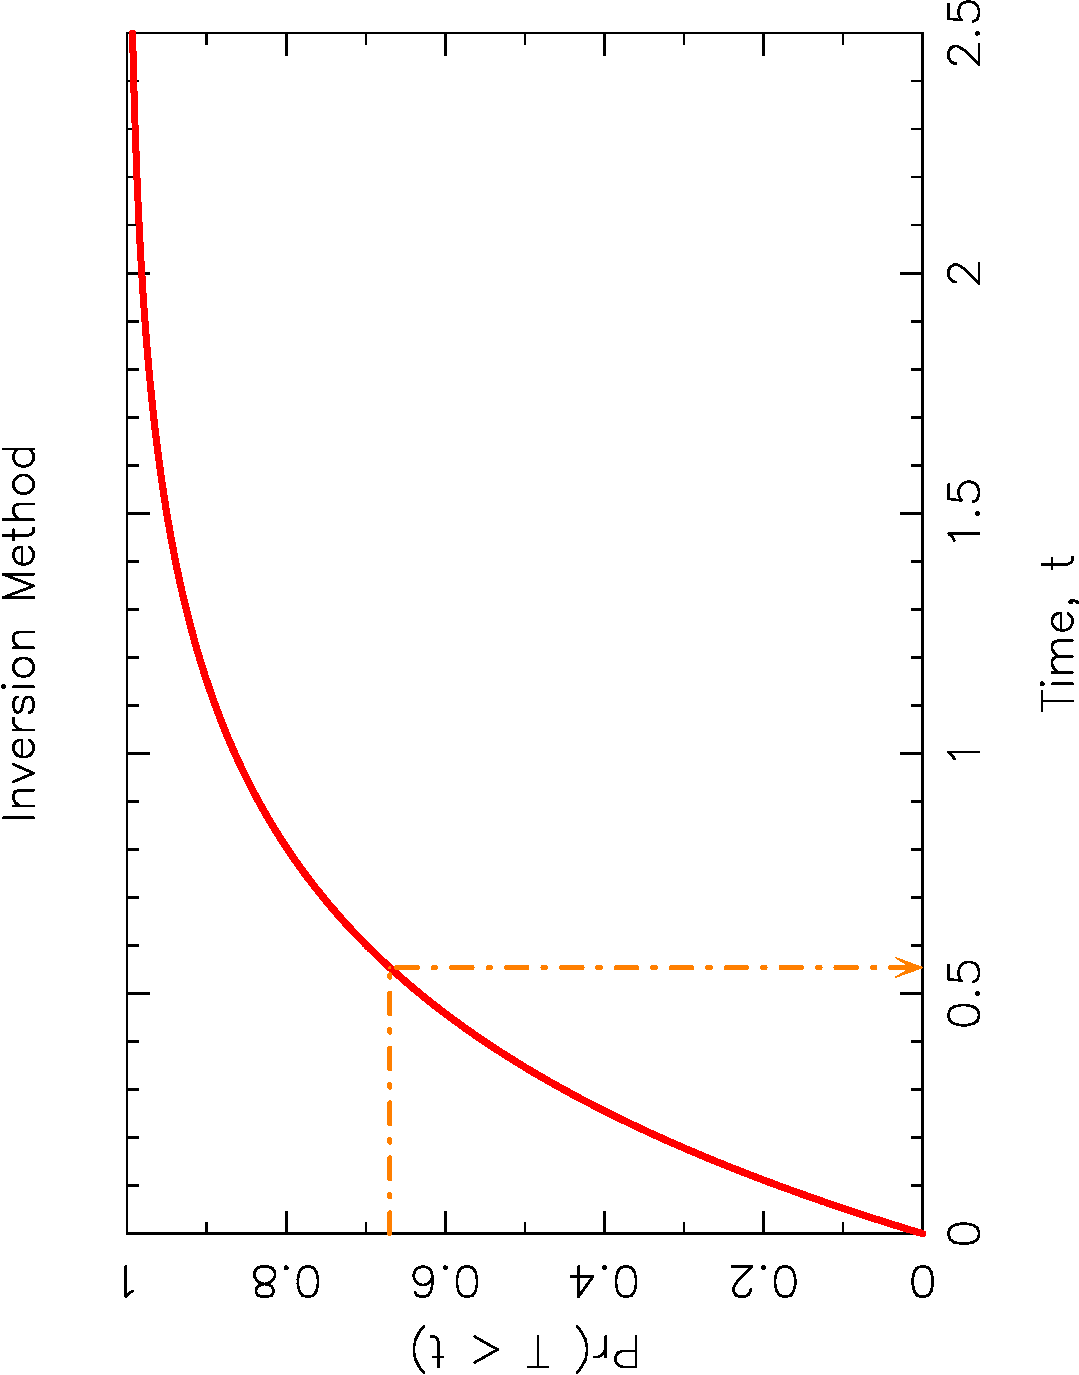
\includegraphics[width=0.6\textwidth,angle=270]{Inversion_Method}
	\caption[Inversion Method]{In order to sample a random variable following a given probability distribution, the inversion method is often used. One generates a uniformly distributed random number between 0 and 1, on the vertical axis, and looks for the corresponding value on the horizontal axis according to the cumulative probability distribution. Here, we have plotted the cumulative distribution function corresponding to an exponentially distributed random variable, $T$, with parameter $\lambda = 2.0$ ---see Eq (\ref{Exponential_Distribution}).}
	\label{Inversion_Method}
\end{figure}

\subsection{Gillespie's Direct Method}
Let us write now an algorithm to generate stochastic replicates in this simple example. This simple algorithm is called Gillespie's direct method.  
The Gillespie algorithm generating a stochastic realization of a Poissonian counting process (up to a maximum number of individuals), under which individuals arrive at an average rate $\lambda$ to a queue, can be summarized as follows:
\begin{enumerate}
	\item Initialize parameter $\lambda$
	\item Initialize a maximum number of individuals $M = 1000$
	\item Initialize the number of individuals in the queue as $n=0$.
	\item Initialize the time $t_0 = 0$
	\item Generate a random number $\Phi$ between 0 and 1. 
	\item Apply Eq (\ref{Random_Time}) to sample an inter-event time $t$. 
	\item Update queue $n \leftarrow n+1$. 
	\item Advance the time, this is, $t_n = t_{n-1} + t$
	\item If $n < M$, then go to 5 otherwise stop
\end{enumerate}
Then, the set $t_0, t_1, \dots, t_M$ is a single realization of the Poissonian counting process defining increasing stochastic times for the $M$ different arrivals.
\smallskip

A counting process is very simple. There is only one type of event that can happen: the arrival of a new individual. We already defined processes where, in addition, individuals can die or reproduce. In order to apply this algorithm, generally, to more complicated stochastic processes where different competing events may change the configuration of the system, we need to carefully understand the meaning of the total rate of something happening within the system. If something happens, it means there is an event that has occurred and, therefore, changed the system configuration. For example, for the Immigration-Death process conforming a \textit{sink} population (see section \ref{Immigration-Death-Process}), we have two different processes: immigrant arrivals and individual deaths. If we have $n$ individuals in the population, as we have discussed, the probability, in some little time $dt$, of a new individual arriving or one of the $n$ individuals dying will be the sum:
\begin{equation} 
\Pb[n \rightarrow n+1] + \Pb[n \rightarrow n-1] = \lambda\,dt + \mu \, n \,dt
\end{equation}
Therefore, the total temporal rate, $R(n)$, is:
\begin{equation} 
R(n) = \lambda + \mu \, n
\end{equation}
\smallskip

Notice the total rate $R(n)$ should account, exhaustively, for all the possible events that can ever happen in the system when it is in certain configuration, in this case, the population has $n$ individuals. While we are waiting for an event to happen, the total rate, $R(n)$, does not change at all, since $n$ is not changing. So, what is the probability that we are still waiting for an event to happen after certain time $t$? This should also be Poissonian because while we are waiting $R(n)$ is fully constant. Therefore, the probability that the system, at certain time $t$, is still waiting for an event to happen, this is, the probability that the next event happens at a time larger than $t$, this is, the time-to-next-event (or inter-event time), $T$, is larger than $t$ should be (see Eq (\ref{Eq_Exp_1})):
\begin{equation}
\Pb\{T>t\} =  e^{-R(n) t}
\end{equation}
and, again, it is crystal clear that:
\begin{equation}
\Pb\{T<t\} =  1 - e^{-R(n) t}
\end{equation}
which means that the time-to-next-event follows an exponential distribution with parameter the total rate $R(n)$. This is the most important point of the general Gillespie algorithm \citep{Gillespie76}. Notice that as the system changes configuration, the inter-event time still follows an exponential distribution but with a different parameter, the new total rate. In particular, imagine a system evolving to a frozen state when nothing else can happen, this is, the total rate of something happing in the system has exactly become zero. Therefore, if $R(n) = 0$, then $\Pb\{T<t\} = 0$ for any $t$ as large as you want, this is, the inter-event time becomes infinite because you can wait and wait but there is no further event to happen.  
\smallskip

Therefore, in order to sample inter-event times, we can safely follow the same strategy as before, this is, we can apply:
\begin{equation}
t     = -\frac{\log(\Phi)}{R(n)}
\label{Random_Time_General}
\end{equation}
but, once the time-to-the-next event has been determined, we should choose which particular event takes place. This should be done in proportion to the probabilities of each and every possible event. More precisely, Gillespie algorithm chooses an event by sampling the discrete probability distribution determined by the set of probabilities associated to each and every possible event in the system. For instance, in our example above, we should choose between either a new arrival or the death of one of the individuals in the system. So, we define two probabilities:
\begin{eqnarray}
p_1 &=& \frac{\lambda}{\lambda + \mu\,n} \nonumber \\
p_2 &=& \frac{\mu\,n}{\lambda + \mu\,n}  \label{p_1p_2}
\end{eqnarray}
and sample either the first (arrival) or the second (death) event accordingly. 
\smallskip

Although the Gillespie algorithm works for any one-step processes in continuous time, I will summarize now how to implement it for the \textit{sink} population above (following Gillespie's direct method):
\begin{enumerate}
	\item Initialize parameters $\lambda$ and $\mu$. 
	\item Initialize a stopping criterion $t_M = 1000$
	\item Initialize the number of individuals in the system as $n=0$.
	\item Initialize the total number of events (or elemental steps) as $i=0$.
	\item Initialize the time $t_0 = 0$
	\item Generate a random number $\Phi$ between 0 and 1.
	\item Update total rate $R(n) = \lambda + \mu\,n$ 
	\item Apply Eq (\ref{Random_Time_General}) to sample an inter-event time $t$.
	\item Update $p_1$ and $p_2$ according to Eqs (\ref{p_1p_2}) 
	\item Sample\footnote{Statistical packages, such as $R$, implement functions to sample efficiently a discrete probability distribution given the set of probabilities associated to each possible event. This function is usually called $sample(\vec{p})$, where $\vec{p}$ is a $m$-dimensional probability vector and returns an index between 1 and $m$ to indicate the selected event.} a new event ($j$) to happen: $j \leftarrow sample(p_1, p_2)$ 
	\item If $j=1$ then update population $n \leftarrow n+1$ otherwise ($j=2$) $n \leftarrow n-1$
	\item Advance total number of steps $i \leftarrow i + 1$
	\item Advance the time, this is, $t_i = t_{i-1} + t$
	\item If $t_i < t_M$, then go to 6 otherwise stop
\end{enumerate}
This algorithm would yield a stochastic trajectory of a \textit{sink} population that increases due to random arrivals and decreases due to random individual deaths until time is greater than $t_M$, this is, it follows an immigration-death process (see section \ref{Immigration-Death-Process}). For more complicated processes, it will be essential to write down an exhaustive table of all possible events with their associated probability rates. In general, for a system whose configuration is defined by a state vector $\vec{n}$, where there are $m$ possible events, we can sketch such a table as:
\begin{center}
	\begin{tabular}{lc}
		\textbf{Event} & \textbf{Event Rate} \\
		
		1          & $R_1(\vec{n})$ \\
		2          & $R_2(\vec{n})$ \\
		$\dots$    & $\dots$        \\
		$m$        & $R_m(\vec{n})$ \\
		           &                \\
		\textbf{Total Rate} & $R(\vec{n}) = \sum_{i=1}^m R_i(\vec{n})$
	\end{tabular}
\end{center}

\subsection{The Immigration-Birth-Death Process: Two Populations}
As an example, let us now write an events table for an immigration-birth-death process of two populations of two different species colonizing the same island. The state of such a system is defined by a two-dimensional state vector, $\vec{n} = (n_1, n_2)$, where $n_1$ and $n_2$ are the number of individuals of the first and second species, respectively. Each species colonizes the island at a species-specific rate ($\lambda_i$, for $i=1,2$), and individuals die and reproduce at species-specific rates ($\mu_i$, for $i=1,2$ $\beta_i$, for $i=1,2$) as well. There are then six possible events, which are summarized in the following events table with their rates:

\begin{center}
	\begin{tabular}{lcc}
		\textbf{Event} & \textbf{Configuration Change} & \textbf{Event Rate}                                                               \\
		
		1      & $n_1 \rightarrow n_1 + 1$ & $R_1(\vec{n}) = \lambda_1$              \\
		2      & $n_1 \rightarrow n_1 + 1$ & $R_2(\vec{n}) = \beta_1\,n_1$           \\
		3      & $n_1 \rightarrow n_1 - 1$ & $R_3(\vec{n}) = \mu_1\,n_1$             \\
		4      & $n_2 \rightarrow n_2 + 1$ & $R_4(\vec{n}) = \lambda_2$              \\
		5      & $n_2 \rightarrow n_2 + 1$ & $R_5(\vec{n}) = \beta_2\,n_2$           \\
		6      & $n_2 \rightarrow n_2 - 1$ & $R_6(\vec{n}) = \mu_2\,n_2$             \\
		       &                           &                                         \\
		       & \textbf{Total Rate}       & $R(\vec{n}) = \sum_{i=1}^6 R_i(\vec{n})$
	\end{tabular}
\end{center}
We can then use the Gillespie algorithm above to generate a stochastic trajectory of the system. All we need is to define the total rate as a sum over the 6 event rates. We also require to define a corresponding 6-dimensional probability vector, $\vec{p}$, again by dividing each event rate by the total rate. Finally, we require to sample this discrete probability distribution to choose an specific event to occur, and update the configuration of the system accordingly (see corresponding configuration change in the table above).  
\smallskip

\subsection{Gillespie's First Reaction Method}
There is another natural way of generating an exact stochastic realization of the same system. So far, in the Direct Method, we have calculated the total rate $R(\vec n)$ in order to sample the time to the next event, and only afterwards have we decided which particular event is going to occur. Could we do both things at once? Indeed, we can. This is the main idea behind Gillespie's \emph{First Reaction Method} \citep{Gillespie76}.
\smallskip

Suppose that, given the current configuration $\vec n$, there are $m$ possible elementary events, each characterized by a rate $R_j(\vec n)$, for $j=1,\ldots,m$. Imagine now that we have $m$ independent clocks running in parallel, one for each possible event. While the configuration remains unchanged, each clock has an exponentially distributed waiting time, with its own rate. For every event whose rate is positive, we independently draw a uniform random number $\Phi_j$ between 0 and 1 and calculate
\begin{equation}
 \tau_j=-\frac{\log\Phi_j}{R_j(\vec n)}, \qquad j=1,\ldots,m.
 \label{First_Reaction_Clocks}
\end{equation}
If an event is impossible in the current configuration, $R_j(\vec n)=0$, we simply assign $\tau_j=\infty$. Of course, among all these prospective waiting times there will be one that is the smallest (ties have probability zero for positive exponential clocks). This is the event that fires first! More precisely, we choose
\begin{equation}
 j^*=\underset{1\leq j\leq m}{\operatorname{arg\,min}}\,\tau_j,
 \qquad \tau=\tau_{j^*}=\min_j\tau_j.
 \label{First_Reaction_Minimum}
\end{equation}
We then advance time by $\tau$ and apply the configuration change associated with event $j^*$. The new configuration may change some, or even all, of the event rates. Therefore, we recalculate the rates, draw a fresh set of prospective waiting times, and repeat the procedure. We are again looking at our system, with several possible stochastic events competing to fire first.
\smallskip

Why is this equivalent to Gillespie's Direct Method? Let us answer this question by recalling a simple property of independent exponential random variables. For a given configuration $\vec n$, the probability that \emph{none} of the $m$ events has occurred before time $t$ is the product
\begin{equation}
 \Pb\{\tau>t\}
 =\prod_{j=1}^{m}\Pb\{\tau_j>t\}
 =\prod_{j=1}^{m}e^{-R_j(\vec n)t}
 =e^{-R(\vec n)t},
 \qquad R(\vec n)=\sum_{j=1}^{m}R_j(\vec n).
 \label{First_Reaction_Survival}
\end{equation}
Thus the minimum waiting time is exponentially distributed with the \emph{total} rate, exactly as in the Direct Method. Furthermore, the probability that event $j$ is the first to occur is
\begin{equation}
 \Pb\{j^*=j\mid\vec n\}
 =\frac{R_j(\vec n)}{R(\vec n)}.
 \label{First_Reaction_Choice}
\end{equation}
So both methods sample the same waiting time and the same event probabilities. The difference is only in how we organize the random draws.
\smallskip

Let us summarize the First Reaction Method for a system with $m$ possible events and state vector $\vec n$:
\begin{enumerate}
 \item Initialize the model parameters, the initial configuration $\vec n$, the initial time $t=0$, and the final simulation time $t_M$.
 \item Calculate the rates $R_j(\vec n)$ for all events $j=1,\ldots,m$.
 \item For every event with $R_j(\vec n)>0$, generate an independent uniform random number $\Phi_j$ and calculate its prospective waiting time $\tau_j$ using Eq.~(\ref{First_Reaction_Clocks}); otherwise set $\tau_j=\infty$.
 \item Find the event $j^*$ with the smallest waiting time $\tau=\tau_{j^*}$.
 \item If every waiting time is infinite, stop: the system has reached a configuration from which no event can occur. If $t+\tau>t_M$, stop at $t_M$ without executing that event.
 \item Otherwise advance the time, $t\leftarrow t+\tau$, and update the configuration according to event $j^*$.
 \item Return to step 2 with the new configuration.
\end{enumerate}

For example, in our immigration--death process there are only two competing events. We draw $\tau_1\sim\mathrm{Exponential}(\lambda)$ for the next immigration and, when $n>0$, $\tau_2\sim\mathrm{Exponential}(\mu n)$ for the next death. If $\tau_1<\tau_2$, an immigrant arrives; otherwise an individual dies. After that, we update the population size and draw both clocks again.
\smallskip

The First Reaction Method is particularly transparent conceptually, but it may be computationally expensive when the number of possible events is very large: at every step we generate up to $m$ waiting times and look for the smallest one. Importantly, the complete resampling of clocks is part of this algorithm. We will see that the Next Reaction Method of Gibson and Bruck \citep{Gibson00}reuses scheduled times and updates them more efficiently, taking advantage of which rates actually change after an event.

\subsection{Efficient simulation of spatially extended stochastic systems} 

\label{space}
Our goal is to extend a model specified for a well-mixed local population to a network of $M$ nodes. As an example, each node will represent a local population undergoing consumer--resource dynamics, and individuals may also move randomly between connected nodes. This spatial extension makes the computational challenge particularly clear: as the number of nodes increases, so does the number of possible stochastic events. However, an event occurring at one node generally changes the transition rates only at that node and, in the case of dispersal, at a neighboring node. The rates in the rest of the network remain unchanged. This local dependence is precisely what efficient algorithms, such as the Next Reaction Method of Gibson and Bruck, exploit through a dependency graph and an event queue. The purpose of this section is to illustrate the importance of this optimization strategy, first through stochastic diffusion and then through a spatially extended consumer--resource model.
\smallskip
   
\subsection*{{\bfseries Stochastic diffusion}}   
 We first introduce a simple stochastic model for a population diffusing on a discrete network where individuals can jump from node to node at a constant rate $\mu$. We consider a constant total population of $n_A$ individuals of a species $A$ distributed over a series of $M$ nodes. The set of nodes defines a metapopulation network where each node host a population at the spatial location $r_i$. We may use generic graphs to characterize the spatial network. The number of individuals in each node of the network at $r_i$ at time $t$ is given by $n(r_i;t)$ with $n \in [0, \dots, n_A]$, $i \in [1,\cdots,M]$, and $t \in \mathbb{R}$, where the total number of nodes is $M$.
\smallskip

Let us introduce a short notation to represent the number of individuals at every node $i$ at time $t$:
\begin{equation}
n_i \equiv n(r_i;t),
\label{eq:spatial_state}
\end{equation}
for $i=1, \dots, M$, which fully determines the configuration of the system at any given time. 
\smallskip

The process is completely defined by the initial number of individuals in each site $n(r_i;0)$ ($i \in [1,\cdots,M]$), and the per capita movement rate of each individual into neighboring nodes as defined by the network topology. We first assume that each individual leaves its current node at a total per-capita rate $\mu$, and then chooses one of the available neighboring nodes. If $n_i$ denotes the number of individuals at node $i$, the total movement rate is
\begin{equation}
R(t) =  \mu \sum_{i=1}^{M} n_i(t)
     = \sum_{i=1}^{M} R_i(t), \qquad R_i(t)=\mu n_i(t),
\label{eq:R_M}
\end{equation}
where $R_i$ is the rate at which an individual leaves node $i$. This expression assumes that every occupied node has at least one possible destination. Let $q_{ij}$ be the probability of choosing node $j$ upon departure from $i$, with $\sum_{j\in\mathcal N_i}q_{ij}=1$. The rate of an individual jump $i\to j$ is then $\mu q_{ij}n_i$. For a uniform choice, $q_{ij}=1/|\mathcal N_i|$. We will distinguish this \emph{total departure rate} from a \emph{per-edge jumping rate} below.  
\smallskip

In general, individual movements can be represented by: 
\begin{eqnarray}
A_i + \emptyset_j & \xrightarrow{\mu} &  \emptyset_i + A_j \label{MovementCapacity}
\end{eqnarray}
where an individual in node $i$ jumps into node $j$ leaving an empty set behind. However, this representation involves that jumps are allowed or not depending on the existence of enough room in the receiving node (empty sites within that node). In other words, if the receiving node if full, i.e., at carrying capacity, movement into it is forbidden. In what follows, for simplicity, we will not assume a carrying capacity for the species that move. In this case, individual movements can simply be represented by: 
\begin{eqnarray}
A_i  & \xrightarrow{\mu} &   A_j \label{Movement}
\end{eqnarray}
where here individuals are assumed to move independently from each other, randomly and passively between nodes. This event produces at change in the configuration of the whole system, affecting both location $i$ and $j$. The individual jumping rate, $\mu$, controls this transition rate:
\begin{equation} 
\label{Tu}
T(n_1, \dots, n_i-1, \dots, n_j+1, \dots, n_M|n_1, \dots, n_i, \dots, n_j, \dots, n_M )  = \mu q_{ij}\,n_i
\end{equation} 

In our Gillespie framework, the total rate, $R$ in Eq (\ref{eq:R_M}), determines the distribution of interevent times between individual movement events. Here, we can use a hierarchical Gillespie algorithm where we first choose a location by sampling a discrete probability distribution, according to the different $R_i$'s, which measure the propensity for each location to undergo a change:
\begin{equation}
\left(\frac{R_1}{R}, \dots, \frac{R_M}{R}\right)
\end{equation}
where $M$ is the total number of nodes. Imagine we have chosen location $i$. Then, it means that that population looses one individual, i.e., it goes from $n_i$ to $n_i-1$. Where does this individual go? In a second step, we choose a location among the neighborhood of the focal one (see Box 2 for details on the hierarchical algorithm). If we have chosen $j$ as a second location, we should update accordingly the $j$-th population, which gains one individual, from $n_j$ to $n_j+1$. 
\smallskip

General network structures can also be implemented without much trouble. An ecological meaningful example assumes a network of nodes (or patches) at a given physical distance, $d_{ij} =|r_j -r_i|$, from each other. Although other dispersal kernels are possibile, we may assume that migration decays exponentially as the between-patch Euclidean distance increases, then a per-capita movement rate assigned to the directed edge from patch $i$ to patch $j$ can be defined as
\begin{equation}
\mu_{ij} = \mu_0 \, e^{-\lambda\,d_{ij}}. \nonumber
\end{equation}
In this case, the total rate given by Eq. (\ref{eq:R_M}) is now written as
\begin{equation}
R(t) = \sum_{i=1}^{M} \hat{\mu}\,(x_i) n(x_i;t),
\label{eq:R_MM}
\end{equation}
where $\hat{\mu}\,(x_i)$ is defined ($\hat{\mu}_i$ for short) as the total per-capita rate of leaving node $i$, namely  
\begin{equation}
\hat{\mu}\,(x_i) = \sum_{j \in {\cal N}_i} \mu_{ij}.
\end{equation}   

If we assume each node occupies the same surface, $S$, we can also define a corresponding density or number of individuals per unit area:   
\begin{equation}
x_i \equiv \frac{n(r_i;t)}{S},
\label{eq:x_i}
\end{equation}

For a square lattice of step size $L$, let us now use the alternative convention that $\mu$ is the rate \emph{per outgoing edge}. Thus, in the interior of a square lattice with four neighbors, the total departure rate is $4\mu n_i$, rather than $\mu n_i$. The evolution of the mean density is described exactly by the following linear equations (for deterministic initial conditions, or with $x_i$ interpreted as the mean density):
\begin{equation}
\frac{dx_i}{dt} = -\hat{\mu}_i\,x_i + \mu \, \sum_{j \in {\cal N}_i} x_j, 
\end{equation}
for $i=1, \dots, M$, where ${\cal N}_i$ is the set of nodes that are connected to the $i$-th node, the neighborhood of each node, and we see that 
\begin{align*}
\hat{\mu}_i   &= \sum_{j \in {\cal N}_i} \mu
\end{align*} 
\begin{align*}
\hat{\mu}_i   &= \mathbf{card}({\cal N}_i)\, \mu
\end{align*} 
for $i=1, \dots, M$. Assuming a Von Neumann neighborhood, this can be simply written as
\begin{equation}
\frac{dx_i}{dt} = 4\,\mu \left(\frac{1}{4} \left[\sum_{j \in {\cal N}_i} x_j\right] - x_i\right)
\end{equation}
for $i=1, \dots, M$. This equation simply says that the rate of increase in the local density of individuals at a location, $r_i$, is proportional to the difference between the average density in a \emph{close} neighborhood around $r_i$, and the local density at that location. Notice that the factor $4\mu$ in the last expression multiplies the difference between the neighbor average and the local density; it is \emph{not} the continuum diffusion coefficient. Indeed, for a smooth spatial density $x(\mathbf r,t)$,
\[
\sum_{j\in\mathcal N_i}x_j-4x_i
  =L^2\,\Delta x(\mathbf r_i,t)+O(L^4).
\]
Therefore, the corresponding continuum diffusion equation is
\begin{equation}
\frac{\partial x}{\partial t} = D\,\Delta x, \qquad D=\mu L^2,
\label{eq:Diffusion}
\end{equation}
where $\Delta$ is the spatial Laplacian. To obtain a nonzero finite diffusion coefficient as $L\to0$, the edge-jumping rate must scale as $\mu=D/L^2$. If instead $\mu$ denotes the total departure rate and each of four neighbors is chosen with probability $1/4$, then $D=\mu L^2/4$. This distinction is important when comparing simulations with continuum reaction--diffusion equations.  
\smallskip

\subsubsection*{The stochastic reaction--diffusion model: a consumer feeding on a logistic-growing resource}
In the order to make this spatial extension, we will consider that searching individuals may move. They may disperse to other local populations at a given rate $\mu_C$. Handling individuals, the ones that reproduce and give rise to searching individuals, will not move. The sensible idea of considering two types of individuals, they ones that move and they ones that reproduce but not move, will be introduced, by symmetry, into the dynamics of the resource population. We will consider that resource reproducing individuals are sessile (they don't move), and produce resource propagules at rate $\beta_R$, while individual propagules do disperse randomly to neighboring local populations, at a rate $\mu_R$ (denoted $\mu_P$ in the event table below). Therefore, symmetrically, we also consider two types of resource individuals, the reproducing and the dispersing ones. Propagules will get eventually established at a rate ($\eta_R$), a process that will be modulated by the amount of empty space in that local population. For completeness, we re-write here the reaction scheme for all the processes involved on a given focal population including the loss and gain of individuals through random movements:   
\begin{center}
\small
\renewcommand{\arraystretch}{1.19}
\begin{tabular}{@{}r p{0.34\linewidth} p{0.28\linewidth} l@{}}
\hline
No. & Elementary event & Reaction scheme & Rate parameter \\
\hline
1 & Out-dispersal of resource propagules & $ P_i \to P_j $ & $ \mu_P $ \refstepcounter{equation}\label{outPopagule} \\
2 & In-dispersal of resource propagules & $ P_j \to P_i $ & $ \text{same event as 1} $ \refstepcounter{equation}\label{inPopagule} \\
3 & Propagule death & $ P \to \emptyset $ & $ \delta_P $ \refstepcounter{equation}\label{PopaguleDeath} \\
4 & Propagule production & $ R \to R+P $ & $ \beta_R $ \refstepcounter{equation}\label{Birth_P} \\
5 & Propagule establishment & $ P+\emptyset \to R $ & $ \eta_R $ \refstepcounter{equation}\label{Establishment_P} \\
6 & Resource death & $ R \to \emptyset $ & $ \delta_R $ \refstepcounter{equation}\label{Death_R} \\
7 & Out-dispersal of searching consumers & $ A_i \to A_j $ & $ \mu_C $ \refstepcounter{equation}\label{outSearching} \\
8 & In-dispersal of searching consumers & $ A_j \to A_i $ & $ \text{same event as 7} $ \refstepcounter{equation}\label{inSearching} \\
9 & Searching consumer death & $ A \to \emptyset $ & $ \delta_A $ \refstepcounter{equation}\label{Death_A} \\
10 & Attack & $ A+R \to A_R+\emptyset $ & $ \alpha $ \refstepcounter{equation}\label{Attack} \\
11 & Handling completion & $ A_R \to A $ & $ \nu $ \refstepcounter{equation}\label{Handling} \\
12 & Consumer reproduction & $ A_R \to A_R+A $ & $ \beta_A $ \refstepcounter{equation}\label{Growth_A} \\
13 & Handling consumer death & $ A_R \to \emptyset $ & $ \delta_A $ \refstepcounter{equation}\label{Death_AR} \\
\hline
\end{tabular}
\end{center}
\noindent The in-dispersal rows (2 and 8) describe the receiving end of the same movement events represented in rows 1 and 7. They must not be counted as additional, independent stochastic events. The table lists the \emph{reaction schemes} and their kinetic parameters; the actual transition rates depend on the current numbers of individuals and, where appropriate, available space. For movement from node $i$ to $j$, the destination is selected according to the dispersal network. Equations below specify the propensities for a focal patch.

Notice the symmetry of the reproduction process of both resources and consumers (see Eq (\ref{Growth_A}) and (\ref{Birth_P})). As explained before, for any out-dispersal event in a focal population there will be a in-dispersal event in a neighboring local population. Here we will prescribe to calculate the total rate of something happening in a focal local population by counting only the out-dispersal processes along with the rest of local processes. We will not count the in-dispersal processes, because these rates depend on the neighboring patches of the focal population and not on the focal patch itself. The state of every local population will be described by four integers $(k,n,m,l)$, where an additional $k$ represents here the number of propagules in that local population. The total rate for a local population to undergo a change of any kind, if it is in a given configuration, $\vec{n}=(k,n,m,l)$, will the sum of the following rates:
\begin{center}
\small
\renewcommand{\arraystretch}{1.18}
\begin{tabular}{@{}r p{0.33\linewidth} p{0.35\linewidth} l@{}}
\hline
No. & Event & Change in focal state & Propensity \\
\hline
1 & Propagule dispersal (departure) & $(k,n,m,l)\to(k-1,n,m,l)$ & $\mu_P k$ \\
3 & Propagule death & $(k,n,m,l)\to(k-1,n,m,l)$ & $\delta_P k$ \\
4 & Propagule production & $(k,n,m,l)\to(k+1,n,m,l)$ & $\beta_R n$ \\
5 & Propagule establishment & $(k,n,m,l)\to(k-1,n+1,m,l)$ & $\eta_R (1-n/N)k$ \\
6 & Resource death & $(k,n,m,l)\to(k,n-1,m,l)$ & $\delta_R n$ \\
7 & Consumer dispersal (departure) & $(k,n,m,l)\to(k,n,m-1,l)$ & $\mu_C m$ \\
9 & Searching consumer death & $(k,n,m,l)\to(k,n,m-1,l)$ & $\delta_A m$ \\
10 & Attack & $(k,n,m,l)\to(k,n-1,m-1,l+1)$ & $\alpha(n/N)m$ \\
11 & Handling completion & $(k,n,m,l)\to(k,n,m+1,l-1)$ & $\nu l$ \\
12 & Consumer reproduction & $(k,n,m,l)\to(k,n,m+1,l)$ & $\beta_A l$ \\
13 & Handling consumer death & $(k,n,m,l)\to(k,n,m,l-1)$ & $\delta_A l$ \\
\hline
\end{tabular}
\end{center}
\noindent Here $k$, $n$, $m$, and $l$ denote resource propagules, established resources, searching consumers, and handling consumers, respectively. For departure events the simultaneous arrival in the selected destination patch is part of the \emph{same} global event. In particular, establishment consumes one propagule; this was omitted from one transition in the original list.
  
Using the notation already explained in a previous section, we may write the analogous expression for the total rate (see Eq (\ref{Rate})) for a given focal population in the configuration state $\vec{n}=(k,n,m,l)$ to undergo any change as:
\begin{equation}
R^j(\vec{n}) = \sum_{i\in\{1,3,4,5,6,7,9,10,11,12,13\}} R^{\textup{out}}_i(\vec{n}_j)
\label{Rate_j}
\end{equation}
where here the superscript and subscipt $j$ emphasizes that this corresonds to the $j-th$ focal population belonging to a network of communities or metacommunity, with $j=1, \dots, M$. We remark also that the {\em in-disperal rates} number 2 and 8 are not considered. The reason is that they are linked to events that have an origin in a neighboring patch, whose rates will be considered when calculating the total rates of those neighboring patches. In that way, as explained in the previous section, the {\em grand} total rate associated to the whole $M$-patch system undergoing any change in any focal patch will safely be the sum of Eq (\ref{Rate_j}) over patches (without counting dispersal processes twice). This will be the {\em grand} total rate controlling the stochastic time, analogous to previous Eq (\ref{eq:R_M}):
\begin{equation}
  R(t) =  \sum_{j=1}^{M} R^j(\vec{n}_j)
  \label{eq:RD_M}
\end{equation}  
 
An implementation may store a matrix of changes in propensities $\mathbf{\Delta r}$ together with auxiliary dependency matrices $\mathbf A$ and $\mathbf T$. The original matrices are retained below as an advanced implementation example; their entries and indexing conventions should be checked against the event representation adopted in the table before they are used as executable specifications. For understanding the main computational idea, it is enough to know which event rates must be updated after each state change.  

\begin{equation}
{\bf T} = 
\left[ \begin{array}{ccc|ccc|ccc|cccc}
1 & 0 & 1  & 0 & 1 & 0  & 0 & 0 & 0  & 0 & 0 & 0 & 0 \\
1 & 0 & 1  & 0 & 1 & 0  & 0 & 0 & 0  & 0 & 0 & 0 & 0 \\
1 & 0 & 1  & 0 & 1 & 0  & 0 & 0 & 0  & 0 & 0 & 0 & 0 \\
\hline
1 & 0 & 1  & 0 & 1 & 0  & 0 & 0 & 0  & 0 & 0 & 0 & 0 \\
1 & 0 & 1  & 1 & 1 & 1  & 0 & 0 & 0  & 1 & 0 & 0 & 0 \\
0 & 0 & 0  & 1 & 1 & 1  & 0 & 0 & 0  & 1 & 0 & 0 & 0 \\
\hline
0 & 0 & 0  & 0 & 0 & 0  & 1 & 0 & 1  & 1 & 0 & 0 & 0 \\
0 & 0 & 0  & 0 & 0 & 0  & 1 & 0 & 1  & 1 & 0 & 0 & 0 \\
0 & 0 & 0  & 0 & 0 & 0  & 1 & 0 & 1  & 1 & 0 & 0 & 0 \\
\hline
0 & 0 & 0  & 1 & 1 & 1  & 1 & 0 & 1  & 1 & 1 & 1 & 1 \\
0 & 0 & 0  & 0 & 1 & 0  & 1 & 0 & 1  & 1 & 1 & 1 & 1 \\
0 & 0 & 0  & 0 & 1 & 0  & 1 & 0 & 1  & 1 & 0 & 0 & 0 \\
0 & 0 & 0  & 0 & 1 & 0  & 0 & 0 & 0  & 0 & 1 & 1 & 1 \\
\end{array}
\right]
\label{T_E}
\end{equation}

As you can see, the second and the eighth column are identically zero because they correspond to changes in immigration rates from neighboring local populations due an event happening in the focal population. Under the assumed source-controlled dispersal rates, changes in the focal population do not change departure rates of individuals located in neighboring populations. This ceases to hold if movement depends on destination occupancy or attractiveness. However, the second and the eighth rows are not zero because they represent the impact of the new incoming immigrant on the rates controlling the events in the focal population.  

\begin{equation}
{\bf A} = 
\left[ \begin{array}{ccc|ccc|ccc|cccc||c}
1 & 3 & 5   & 0 & 0 & 0  & 0 & 0 & 0  & 0 & 0 & 0 & 0 & 3\\
1 & 3 & 5   & 0 & 0 & 0  & 0 & 0 & 0  & 0 & 0 & 0 & 0 & 3\\
1 & 3 & 5   & 0 & 0 & 0  & 0 & 0 & 0  & 0 & 0 & 0 & 0 & 3\\
\hline
1 & 3 & 5   & 0  & 0 & 0   & 0 & 0 & 0  & 0 & 0 & 0 & 0 & 3\\
1 & 3 & 4   & 5  & 6 & 10  & 0 & 0 & 0  & 0 & 0 & 0 & 0 & 6\\
4 & 5 & 6   & 10 & 0 & 0   & 0 & 0 & 0  & 0 & 0 & 0 & 0 & 4\\
\hline
7 & 9 & 10  & 0 & 0 & 0  & 0 & 0 & 0  & 0 & 0 & 0 & 0 & 3\\
7 & 9 & 10  & 0 & 0 & 0  & 0 & 0 & 0  & 0 & 0 & 0 & 0 & 3\\
7 & 9 & 10  & 0 & 0 & 0  & 0 & 0 & 0  & 0 & 0 & 0 & 0 & 3\\
\hline
4  & 5  & 6   & 7  & 9  & 10  & 11 & 12 & 13  & 0 & 0 & 0 & 0 & 9\\
7  & 9  & 10  & 11 & 12 & 13  & 0 & 0 & 0     & 0 & 0 & 0 & 0 & 6\\
7  & 9  & 10  & 0  & 0  & 0   & 0 & 0 & 0     & 0 & 0 & 0 & 0 & 3\\
11 & 12 & 13  & 0  & 0  & 0   & 0 & 0 & 0     & 0 & 0 & 0 & 0 & 3\\
\end{array}
\right]
\label{A_E}
\end{equation}

They are, on average, 4 rates that are changed as a result of an event happening in the focal population. Thus, relatively few local propensities need to be updated after a typical event, compared with a naive algorithm that recalculates all local rates from scratch. The exact computational gain depends on data structures, network connectivity and the cost of updating scheduled times. In addition, when an event occurs in a patch, which does not involve movement of individuals, only the rates in that patch change. If the occurring event is the 1 or the 7, which involve movement of propagules or searching individuals, respectively, then both the rates of that focal patch and the rates of the patch receiving immigrants may be affected, which again leaves the rates in all the other patches totally unchanged. This will involve a tremendous gain in computational time. As $M$ increases, a straightforward algorithm that naively updated the total rate over the whole $M$-patch system from scratch after the occurrence of any event will be computationally unaffordable.   
  
\begin{center}
\begin{sideways}
\begin{minipage}{\textheight}
\begin{equation}
{\bf \Delta r} = 
\left[ \begin{array}{ccc|ccc|ccc|cccc}
-\mu_P & 0 & -\delta_P   & 0 & -\eta_R\,\frac{N-n'}{N} & 0  & 0 & 0 & 0  & 0 & 0 & 0 & 0 \\
 \mu_P & 0 &  \delta_P   & 0 &  \eta_R\,\frac{N-n'}{N} & 0  & 0 & 0 & 0  & 0 & 0 & 0 & 0 \\
-\mu_P & 0 & -\delta_P   & 0 & -\eta_R\,\frac{N-n'}{N} & 0  & 0 & 0 & 0  & 0 & 0 & 0 & 0 \\
\hline
 \mu_P & 0  &  \delta_P   & 0        & \eta_R\,\frac{N-n'}{N}          & 0          & 0 & 0 & 0  & 0                   & 0 & 0 & 0  \\
-\mu_P & 0  & -\delta_P   &  \beta_R & -\frac{\eta_R}{N}(1+k'+(N-n'))  &  \delta_R  & 0 & 0 & 0  & \alpha\frac{m'}{N}  & 0 & 0 & 0 \\
 0     & 0  &  0          & -\beta_R & \eta_R\,\frac{k'}{N}            & -\delta_R  & 0 & 0 & 0  & -\alpha\frac{m'}{N} & 0 & 0 & 0 \\
\hline
0 & 0 & 0                 & 0 & 0 & 0                                              & -\mu_A & 0 & -\delta_A     & -\alpha\,\frac{n'}{N}       &  0   &  0       &  0 \\
0 & 0 & 0                 & 0 & 0 & 0                                              &  \mu_A & 0 &  \delta_A     &  \alpha\,\frac{n'}{N}       &  0   &  0       &  0 \\
0 & 0 & 0                 & 0 & 0 & 0                                              & -\mu_A & 0 &  -\delta_A     & -\alpha\,\frac{n'}{N}       &  0   &  0       &  0 \\
\hline
0 & 0 & 0                 & -\beta_R & \eta_R\frac{k'}{N}              & -\delta_R   & -\mu_A & 0 & -\delta_A     & -\frac{\alpha}{N}(1+n'+m') &  \nu &  \beta_A &  \delta_A  \\
0 & 0 & 0                 & 0 & 0 & 0                                              &  \mu_A & 0 &  \delta_A     & \alpha\,\frac{n'}{N}        & -\nu & -\beta_A & -\delta_A  \\
0 & 0 & 0                 & 0 & 0 & 0                                              &  \mu_A & 0 &  \delta_A     & \alpha\,\frac{n'}{N}        &  0   &  0       &  0         \\
0 & 0 & 0                 & 0 & 0 & 0                                              & 0      & 0 &  0            & 0                          & -\nu & -\beta_A & -\delta_A  \\
\end{array}
\right]
\label{Delta_E}
\end{equation}
\end{minipage}
\end{sideways}
\end{center}

\subsubsection*{The master equation and the macroscopic law}
The transition rates control the temporal evolution of the probability that the system is in a given configuration, $(n,m,l,k)$. On the one hand, we have already calculated the total rate at which the system leaves this state (see Eq (\ref{Rate})). On the other, we can also calculate the total rate at which the system falls in this state from other possible states. The balance between these two (in- and out-) overall processes control the evolution of the whole probability distribution $P(n,m,l,k; t)$. This can be represented by master equation of the system. In our example, we can write: 
\begin{equation}
	\frac{dP(\vec{n}; t)}{dt} = \sum_{i=1}^m R^{\textup{in}}_i(\vec{n}')P(\vec{n}';t) - R^{\textup{out}}(\vec{n})\,P(\vec{n}; t)
	\label{eq:ME}
\end{equation} 
where $R^{\textup{out}}(\vec{n})$ is given by Eq (\ref{Rate}), but here the superscript  emphasizes it is the total out-rate from a general configuration $\vec{n}=(n,m,l,k)$. For every  transition rate in Eqs (\ref{T1})-(\ref{T7}), we can write the corresponding transition rate at which the system falls in that state ($\vec{n}=(n,m,l,k)$). This equation governs the temporal evolution of the probability that the system occupies the various configurations within a given local population, in the absence of diffusion..

We also give the macroscopic law for the dynamics of this model on a single patch, which we analyze and compare to that of the basic model in the next section. We use the same prescriptions and definitions as we did for the basic model represented by Eqs (\ref{eq:x})-(\ref{eq:z}):
\begin{eqnarray}
\label{eq:ww}
\frac{dw}{d\tau}   & = & -d_P \,w + b_R\,x - e_R\,(1-x)\,w \\
\label{eq:xx}
\frac{dx}{d\tau}   & = & -d_R \,x + e_R\,(1-x)\,w -a\,x\,y \\
\label{eq:yy}
\frac{dy}{d\tau}   & = & -d_C \,y + u\,z + b_C\,z -a\,x\,y \\
\label{eq:zz}
\frac{dz}{d\tau}   & = & -d_C \,z + a\,x\,y -u\,z 
\end{eqnarray}
where again $d_R$ is equal to one by definition, and $e_R=\eta_R/\delta_R$, and $d_P = \delta_P/\delta_R$ are new dimensionless parameters, the establishment rate, and the propagule death rate, respectively. The rest of dimensionless parameters have been already defined. Interestingly, as we will see, the fixed points of this extended model, when considered only on one single patch, can be formally re-written in the same way as the ones for the basic model. Not surprisingly, both models show the same qualitative dynamics with some interesting differences we highlight in the next section. Assuming a Von Neumann neighborhood on a grid from $i=1$ to $M$ nodes, the deterministic analog of the stochastic spatially extended system is decribed by: 
\begin{eqnarray}
\label{eq:wwsd}
\frac{dw_i}{d\tau}   & = & -d_P \,w_i + b_R\,x_i - e_R\,(1-x_i)\,w_i + 4\,m_R \left(\frac{1}{4} \left[\sum_{j \in {\cal N}_i} w_j\right] - w_i\right)\\
\label{eq:xxsd}
\frac{dx_i}{d\tau}   & = & -d_R \,x_i + e_R\,(1-x_i)\,w_i -a\,x_i\,y_i \\
\label{eq:yysd}
\frac{dy_i}{d\tau}   & = & -d_C \,y_i + u\,z_i + b_C\,z_i -a\,x_i\,y_i + 4\,m_C \left(\frac{1}{4} \left[\sum_{j \in {\cal N}_i} y_j\right] - y_i\right)\\
\label{eq:zzsd}
\frac{dz_i}{d\tau}   & = & -d_C \,z_i + a\,x_i\,y_i -u\,z_i 
\end{eqnarray}

Finally, in clear analogy to the diffusion equation (Eq.~(\ref{eq:Diffusion})), the continuum spatial model reads (with $D_R=m_RL^2$ and $D_C=m_CL^2$ for per-edge rates on a square lattice): 
\begin{eqnarray}
\label{eq:wws}
\frac{dw}{d\tau}   & = & -d_P \,w + b_R\,x - e_R\,(1-x)\,w + D_R \, \Delta w\\
\label{eq:xxs}
\frac{dx}{d\tau}   & = & -d_R \,x + e_R\,(1-x)\,w -a\,x\,y \\
\label{eq:yys}
\frac{dy}{d\tau}   & = & -d_C \,y + u\,z + b_C\,z -a\,x\,y + D_C \, \Delta y\\
\label{eq:zzs}
\frac{dz}{d\tau}   & = & -d_C \,z + a\,x\,y -u\,z 
\end{eqnarray}
where $m_C \equiv \mu_C/\delta_R$ and $m_R \equiv \mu_R/\delta_R$ are dimensionless movement rates in the lattice equations. Here $D_R$ and $D_C$ are the associated dimensionless continuum diffusion coefficients when spatial coordinates retain units of length. If $\mu_C$ and $\mu_R$ are defined instead as total departure rates (with uniformly chosen neighbors), the coefficients have an additional factor $1/4$. The stability analysis of the full reaction-diffusion system is an interesting question on its own to be addressed in future work.  

\subsection{Gibson and Bruck's Next Reaction Method}

\section{Exact Stochastic Simulation Algorithms}

\subsection{Exponential waiting times and competing stochastic events}
So far we have made a strong emphasis on the correspondence between the deterministic and the stochastic description of the temporal dynamics of a system. The Gillespie algorithm is a robust method to generate stochastic replicates of the temporal dynamics of a system. Suppose we deal with a single population described by the stochastic variable $N$, number of individuals. The method is exact in the sense that it generates realizations of the continuous-time Markov process defined by the prescribed elementary events and their transition rates. For the linear processes discussed so far, averaging over many independent stochastic realizations recovers the deterministic equation for the mean population size. In nonlinear systems, however, the equation for the mean may involve higher moments, so the usual deterministic approximation need not coincide with the exact stochastic mean. Individual stochastic trajectories fluctuate around, and sometimes depart substantially from, deterministic predictions.  
\smallskip

As described in section \ref{subsection:Poisson_Process}, let us assume we have a Poissonian counting process. The line in front the counter keeps increasing due to the constant arrival of individuals at rate $\lambda$. Can we generate stochastic replicates of this process? Of course, we can. We will do it by introducing the Gillespie algorithm. Assuming that there were no individuals at the initial time $t=0$, we know that the number of individuals at a certain time $t$ follows a Poissonian distribution:
\begin{equation}
\Pb(n, t) =  \frac{(\lambda t)^n}{n!} e^{-\lambda t}
\label{Poisson_Distribution}
\end{equation}

Interestingly, there is some non-null probability of having still no individuals after a given time $t$:
\begin{equation}
\Pb(0, t) =  e^{-\lambda t}
\label{Eq_Exp_1}
\end{equation}
which is obtained by making $n=0$ in Eq (\ref{Poisson_Distribution}). The time between two consecutive arrival events can be considered a stochastic variable $T$, which we call the inter-event time.  Since at time $t$ we still have 0 individuals, $\Pb(0, t)$ can be read as the probability that the next arrival occurs at a time larger than $t$. We can then write:
\begin{equation}
\Pb\{T>t\} =  e^{-\lambda t}
\end{equation}
It is also crystal clear that:
\begin{equation}
\Pb\{T<t\} =  1 - e^{-\lambda t}
\end{equation}
Now compare please the last equation with Eq (\ref{Exponential_Distribution}). This comparison is conclusive: $T \sim Exponential(\lambda)$, this is, in words, we can conclude that the stochastic variable $T$, defined as the inter-event time (a.k.a the time-to-the-next-event) follows an exponential distribution of parameter $\lambda$. 
\smallskip

If we know that a random variable follows certain distribution, we can always sample it, i.e., we can use this distribution to draw an individual realization of that variable. When the stochastic variable is continuous, as it is the case for the inter-event time, we can always take a single realization of this stochastic variable by using the so-called inversion method (see Fig \ref{Inversion_Method}). This method uses the cumulative probability distribution (Eq (\ref{Exponential_Distribution})). It draws first a full, uniformly-distributed random number, $\xi$, between 0 and 1, and then, it looks at the time on the horizontal axis that corresponds to this random $\xi$ on the vertical axis\footnote{Here, a full random number, $\xi$, between 0 and 1 means the realization of a stochastic variable, $X$, that follows the uniform distribution between 0 and 1. The cumulative probability distribution of a uniformly distributed random variable, $X$, is then the identity function between 0 and 1, $F(x) = \Pb\{X\,<\,x\}= x$.}  (see Fig \ref{Inversion_Method}). Luckily this can be calculated:
\begin{align*}
 \xi            &= 1 - e^{-\lambda t}            \\
 e^{-\lambda t} &= 1 - \xi                       \\
 -\lambda t     &= \log(1 - \xi)                 \\
          t     &= -\frac{\log(1 - \xi)}{\lambda}
\end{align*}
If $\xi$ is uniformly distributed between 0 and 1, the complementary variable $1-\xi$ will be also uniformly distributed between 0 and 1. We safely define $\Phi \equiv 1-\xi$:
\begin{equation}
 t     = -\frac{\log(\Phi)}{\lambda}
 \label{Random_Time}
\end{equation}

\begin{figure}[t!]
	\centering
	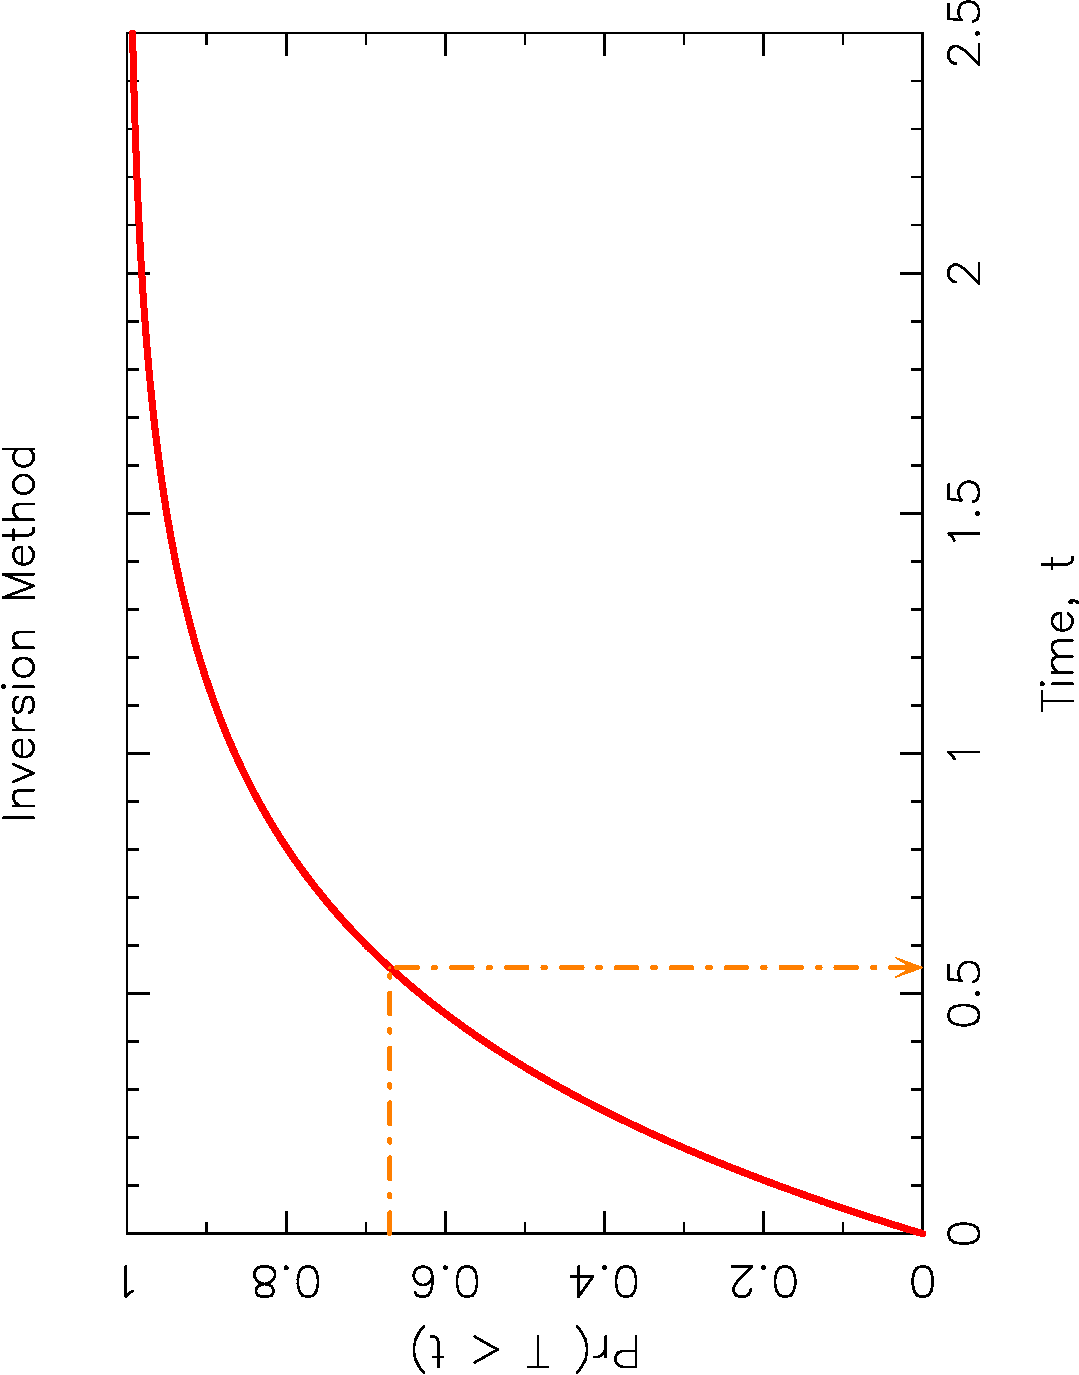
\includegraphics[width=0.6\textwidth,angle=270]{Inversion_Method}
	\caption[Inversion Method]{In order to sample a random variable following a given probability distribution, the inversion method is often used. One generates a uniformly distributed random number between 0 and 1, on the vertical axis, and looks for the corresponding value on the horizontal axis according to the cumulative probability distribution. Here, we have plotted the cumulative distribution function corresponding to an exponentially distributed random variable, $T$, with parameter $\lambda = 2.0$ ---see Eq (\ref{Exponential_Distribution}).}
	\label{Inversion_Method}
\end{figure}

\subsection{Gillespie's Direct Method}
Let us write now an algorithm to generate stochastic replicates in this simple example. This simple algorithm is called Gillespie's direct method.  
The Gillespie algorithm generating a stochastic realization of a Poissonian counting process (up to a maximum number of individuals), under which individuals arrive at an average rate $\lambda$ to a queue, can be summarized as follows:
\begin{enumerate}
	\item Initialize parameter $\lambda$
	\item Initialize a maximum number of individuals $M = 1000$
	\item Initialize the number of individuals in the queue as $n=0$.
	\item Initialize the time $t_0 = 0$
	\item Generate a random number $\Phi$ between 0 and 1. 
	\item Apply Eq (\ref{Random_Time}) to sample an inter-event time $t$. 
	\item Update queue $n \leftarrow n+1$. 
	\item Advance the time, this is, $t_n = t_{n-1} + t$
	\item If $n < M$, then go to 5 otherwise stop
\end{enumerate}
Then, the set $t_0, t_1, \dots, t_M$ is a single realization of the Poissonian counting process defining increasing stochastic times for the $M$ different arrivals.
\smallskip

A counting process is very simple. There is only one type of event that can happen: the arrival of a new individual. We already defined processes where, in addition, individuals can die or reproduce. In order to apply this algorithm, generally, to more complicated stochastic processes where different competing events may change the configuration of the system, we need to carefully understand the meaning of the total rate of something happening within the system. If something happens, it means there is an event that has occurred and, therefore, changed the system configuration. For example, for the Immigration-Death process conforming a \textit{sink} population (see section \ref{Immigration-Death-Process}), we have two different processes: immigrant arrivals and individual deaths. If we have $n$ individuals in the population, as we have discussed, the probability, in some little time $dt$, of a new individual arriving or one of the $n$ individuals dying will be the sum:
\begin{equation} 
\Pb[n \rightarrow n+1] + \Pb[n \rightarrow n-1] = \lambda\,dt + \mu \, n \,dt
\end{equation}
Therefore, the total temporal rate, $R(n)$, is:
\begin{equation} 
R(n) = \lambda + \mu \, n
\end{equation}
\smallskip

Notice the total rate $R(n)$ should account, exhaustively, for all the possible events that can ever happen in the system when it is in certain configuration, in this case, the population has $n$ individuals. While we are waiting for an event to happen, the total rate, $R(n)$, does not change at all, since $n$ is not changing. So, what is the probability that we are still waiting for an event to happen after certain time $t$? This should also be Poissonian because while we are waiting $R(n)$ is fully constant. Therefore, the probability that the time-to-next-event, $T$, is larger than $t$ should be (see Eq (\ref{Eq_Exp_1})):
\begin{equation}
\Pb\{T>t\} =  e^{-R(n) t}
\end{equation}
and, again, it is crystal clear that:
\begin{equation}
\Pb\{T<t\} =  1 - e^{-R(n) t}
\end{equation}
which means that the time-to-next-event follows an exponential distribution with parameter the total rate $R(n)$. This is the most important point of the general Gillespie algorithm \citep{Gillespie76}. Notice that as the system changes configuration, the inter-event time still follows an exponential distribution but with a different parameter, the new total rate. In particular, imagine a system evolving to a frozen state when nothing else can happen, this is, the total rate of something happening in the system has exactly become zero. Therefore, if $R(n) = 0$, then $\Pb\{T<t\} = 0$ for any $t$ as large as you want, this is, the inter-event time becomes infinite because you can wait and wait but there is no further event to happen.  
\smallskip

Therefore, in order to sample inter-event times, we can safely follow the same strategy as before, this is, we can apply:
\begin{equation}
t     = -\frac{\log(\Phi)}{R(n)}
\label{Random_Time_General}
\end{equation}
but, once the time-to-the-next-event has been determined, we should choose which particular event takes place. This should be done in proportion to the probabilities of each and every possible event. More precisely, Gillespie algorithm chooses an event by sampling the discrete probability distribution determined by the set of probabilities associated to each and every possible event in the system. For instance, in our example above, we should choose between either a new arrival or the death of one of the individuals in the system. So, we define two probabilities:
\begin{eqnarray}
p_1 &=& \frac{\lambda}{\lambda + \mu\,n} \nonumber \\
p_2 &=& \frac{\mu\,n}{\lambda + \mu\,n}  \label{p_1p_2}
\end{eqnarray}
and sample either the first (arrival) or the second (death) event accordingly. 
\smallskip

Although the Gillespie algorithm works for any one-step processes in continuous time, I will summarize now how to implement it for the \textit{sink} population above (following Gillespie's direct method):
\begin{enumerate}
	\item Initialize parameters $\lambda$ and $\mu$. 
	\item Initialize a final simulation time $t_M = 1000$
	\item Initialize the number of individuals in the system as $n=0$.
	\item Initialize the total number of events (or elemental steps) as $i=0$.
	\item Initialize the time $t_0 = 0$
	\item Generate a random number $\Phi$ between 0 and 1.
	\item Update total rate $R(n) = \lambda + \mu\,n$ 
	\item Apply Eq (\ref{Random_Time_General}) to sample an inter-event time $t$.
	\item Update $p_1$ and $p_2$ according to Eqs (\ref{p_1p_2}) 
	\item Sample\footnote{Statistical packages, such as $R$, implement functions to sample efficiently a discrete probability distribution given the set of probabilities associated to each possible event. This function is usually called $sample(\vec{p})$, where $\vec{p}$ is a $m$-dimensional probability vector and returns an index between 1 and $m$ to indicate the selected event.} a new event ($j$) to happen: $j \leftarrow sample(p_1, p_2)$ 
	\item If $j=1$ then update population $n \leftarrow n+1$ otherwise ($j=2$) $n \leftarrow n-1$
	\item Advance total number of steps $i \leftarrow i + 1$
	\item Advance the time, this is, $t_i = t_{i-1} + t$
	\item If $t_i < t_M$, then go to 6; otherwise stop (or discard the last event if the trajectory must end exactly at $t_M$)
\end{enumerate}
This algorithm would yield a stochastic trajectory of a \textit{sink} population that increases due to random arrivals and decreases due to random individual deaths up to the prescribed simulation horizon $t_M$, this is, it follows an immigration-death process (see section \ref{Immigration-Death-Process}). For more complicated processes, it will be essential to write down an exhaustive table of all possible events with their associated probability rates. In general, for a system whose configuration is defined by a state vector $\vec{n}$, where there are $m$ possible events, we can sketch such a table as:
\begin{center}
	\begin{tabular}{lc}
		\textbf{Event} & \textbf{Event Rate} \\
		
		1          & $R_1(\vec{n})$ \\
		2          & $R_2(\vec{n})$ \\
		$\dots$    & $\dots$        \\
		$m$        & $R_m(\vec{n})$ \\
		           &                \\
		\textbf{Total Rate} & $R(\vec{n}) = \sum_{i=1}^m R_i(\vec{n})$
	\end{tabular}
\end{center}

\subsection{The Immigration-Birth-Death Process: Two Populations}
As an example, let us now write an events table for an immigration-birth-death process of two populations of two different species colonizing the same island. The state of such a system is defined by a two-dimensional state vector, $\vec{n} = (n_1, n_2)$, where $n_1$ and $n_2$ are the number of individuals of the first and second species, respectively. Each species colonizes the island at a species-specific rate ($\lambda_i$, for $i=1,2$), and individuals die and reproduce at species-specific rates ($\mu_i$ and $\beta_i$, for $i=1,2$) as well. There are then six possible events, which are summarized in the following events table with their rates:

\begin{center}
	\begin{tabular}{lcc}
		\textbf{Event} & \textbf{Configuration Change} & \textbf{Event Rate}                                                               \\
		
		1      & $n_1 \rightarrow n_1 + 1$ & $R_1(\vec{n}) = \lambda_1$              \\
		2      & $n_1 \rightarrow n_1 + 1$ & $R_2(\vec{n}) = \beta_1\,n_1$           \\
		3      & $n_1 \rightarrow n_1 - 1$ & $R_3(\vec{n}) = \mu_1\,n_1$             \\
		4      & $n_2 \rightarrow n_2 + 1$ & $R_4(\vec{n}) = \lambda_2$              \\
		5      & $n_2 \rightarrow n_2 + 1$ & $R_5(\vec{n}) = \beta_2\,n_2$           \\
		6      & $n_2 \rightarrow n_2 - 1$ & $R_6(\vec{n}) = \mu_2\,n_2$             \\
		       &                           &                                         \\
		       & \textbf{Total Rate}       & $R(\vec{n}) = \sum_{i=1}^6 R_i(\vec{n})$
	\end{tabular}
\end{center}
We can then use the Gillespie algorithm above to generate a stochastic trajectory of the system. All we need is to define the total rate as a sum over the 6 event rates. We also require to define a corresponding 6-dimensional probability vector, $\vec{p}$, again by dividing each event rate by the total rate. Finally, we require to sample this discrete probability distribution to choose a specific event to occur, and update the configuration of the system accordingly (see corresponding configuration change in the table above).  
\smallskip

\subsection{Gillespie's First Reaction Method}
There is another natural way of generating an exact stochastic realization of the same system. So far, in the Direct Method, we have calculated the total rate $R(\vec n)$ in order to sample the time to the next event, and only afterwards have we decided which particular event is going to occur. Could we do both things at once? Indeed, we can. This is the main idea behind Gillespie's \emph{First Reaction Method} \citep{Gillespie76}.
\smallskip

Suppose that, given the current configuration $\vec n$, there are $m$ possible elementary events, each characterized by a rate $R_j(\vec n)$, for $j=1,\ldots,m$. Imagine now that we have $m$ independent clocks running in parallel, one for each possible event. While the configuration remains unchanged, each clock has an exponentially distributed waiting time, with its own rate. For every event whose rate is positive, we independently draw a uniform random number $\Phi_j$ between 0 and 1 and calculate
\begin{equation}
 \tau_j=-\frac{\log\Phi_j}{R_j(\vec n)}, \qquad j=1,\ldots,m.
 \label{First_Reaction_Clocks}
\end{equation}
If an event is impossible in the current configuration, $R_j(\vec n)=0$, we simply assign $\tau_j=\infty$. Of course, among all these prospective waiting times there will be one that is the smallest (also, in a way, the most probable to happen first). This is the event that fires first! More precisely, we choose
\begin{equation}
 j^*=\underset{1\leq j\leq m}{\operatorname{arg\,min}}\,\tau_j,
 \qquad \tau=\tau_{j^*}=\min_j\tau_j.
 \label{First_Reaction_Minimum}
\end{equation}
We then advance time by $\tau$ and apply the configuration change associated with event $j^*$. The new configuration may change some, or even all, of the event rates. Therefore, we recalculate the rates, draw a fresh set of prospective waiting times, and repeat the procedure. We are again looking at our system, with several possible stochastic events competing to fire first.
\smallskip

Why is this equivalent to Gillespie's Direct Method? Let us answer this question by recalling a simple property of independent exponential random variables. For a given configuration $\vec n$, the probability that \emph{none} of the $m$ events has occurred before time $t$ is the product
\begin{equation}
 \Pb\{\tau>t\}
 =\prod_{j=1}^{m}\Pb\{\tau_j>t\}
 =\prod_{j=1}^{m}e^{-R_j(\vec n)t}
 =e^{-R(\vec n)t},
 \qquad R(\vec n)=\sum_{j=1}^{m}R_j(\vec n).
 \label{First_Reaction_Survival}
\end{equation}
Thus the minimum waiting time is exponentially distributed with the \emph{total} rate, exactly as in the Direct Method. Furthermore, the probability that event $j$ is the first to occur is
\begin{equation}
 \Pb\{j^*=j\mid\vec n\}
 =\frac{R_j(\vec n)}{R(\vec n)}.
 \label{First_Reaction_Choice}
\end{equation}
So both methods sample the same waiting time and the same event probabilities. The difference is only in how we organize the random draws.
\smallskip

Let us summarize the First Reaction Method for a system with $m$ possible events and state vector $\vec n$:
\begin{enumerate}
 \item Initialize the model parameters, the initial configuration $\vec n$, the initial time $t=0$, and the final simulation time $t_M$.
 \item Calculate the rates $R_j(\vec n)$ for all events $j=1,\ldots,m$.
 \item For every event with $R_j(\vec n)>0$, generate an independent uniform random number $\Phi_j$ and calculate its prospective waiting time $\tau_j$ using Eq.~(\ref{First_Reaction_Clocks}); otherwise set $\tau_j=\infty$.
 \item Find the event $j^*$ with the smallest waiting time $\tau=\tau_{j^*}$.
 \item If every waiting time is infinite, stop: the system has reached a configuration from which no event can occur. If $t+\tau>t_M$, stop at $t_M$ without executing that event.
 \item Otherwise advance the time, $t\leftarrow t+\tau$, and update the configuration according to event $j^*$.
 \item Return to step 2 with the new configuration.
\end{enumerate}

For example, in our immigration--death process there are only two competing events. We draw $\tau_1\sim\mathrm{Exponential}(\lambda)$ for the next immigration and, when $n>0$, $\tau_2\sim\mathrm{Exponential}(\mu n)$ for the next death. If $\tau_1<\tau_2$, an immigrant arrives; otherwise an individual dies. After that, we update the population size and draw both clocks again.
\smallskip

The First Reaction Method is particularly transparent conceptually, but it may be computationally expensive when the number of possible events is very large: at every step we generate up to $m$ waiting times and look for the smallest one. Importantly, the complete resampling of clocks is part of this algorithm. We will see that the Next Reaction Method of Gibson and Bruck \cite{Gibson00}reuses scheduled times and updates them more efficiently, taking advantage of which rates actually change after an event.

\subsection{Gibson and Bruck's Next Reaction Method}
The Next Reaction Method, introduced by  \cite{GibsonBruck2000}, is an efficient modification of Gillespie's First Reaction Method, particularly useful for systems involving a large number of possible stochastic events. The key idea is that, after an event occurs, it is not necessary to recalculate all transition rates or generate a new set of waiting times, since the occurrence of a particular event generally affects only a subset of the other possible events. This is especially important in spatially extended systems, where events occurring at a given location typically modify only the rates associated with that location and its immediate neighbors. The algorithm exploits this property through a {\em dependency graph}, which identifies the events whose rates must be updated, and an efficient priority queue, which keeps track of the scheduled occurrence times and allows the next event to be identified rapidly. The scheduled times of events whose rates change are appropriately adjusted, while unaffected events retain their scheduled times. In this way, the algorithm generates exact realizations of the underlying continuous-time stochastic process while considerably reducing the computational effort required for systems with many events and sparse dependencies.

%\subsection{Efficient simulation of spatially extended stochastic systems} as an input file!!!
\subsection{Efficient simulation of spatially extended stochastic systems}
\label{space}
Our goal is to extend a model specified for a well-mixed local population to a network of $M$ nodes. As an example, each node will represent a local population undergoing consumer--resource dynamics, and individuals may also move randomly between connected nodes. This spatial extension makes the computational challenge particularly clear: as the number of nodes increases, so does the number of possible stochastic events. However, an event occurring at one node generally changes the transition rates only at that node and, in the case of dispersal, at a neighboring node. The rates in the rest of the network remain unchanged. This local dependence is precisely what efficient algorithms, such as the Next Reaction Method of Gibson and Bruck, exploit through a dependency graph and an event queue. The purpose of this section is to illustrate the importance of this optimization strategy, first through stochastic diffusion and then through a spatially extended consumer--resource model.
\smallskip
   
\subsection*{{\bfseries Stochastic diffusion}}   
 We first introduce a simple stochastic model for a population diffusing on a discrete network where individuals can jump from node to node at a constant rate $\mu$. We consider a constant total population of $n_A$ individuals of a species $A$ distributed over a series of $M$ nodes. The set of nodes defines a metapopulation network where each node host a population at the spatial location $r_i$. We may use generic graphs to characterize the spatial network. The number of individuals in each node of the network at $r_i$ at time $t$ is given by $n(r_i;t)$ with $n \in [0, \dots, n_A]$, $i \in [1,\cdots,M]$, and $t \in \mathbb{R}$, where the total number of nodes is $M$.
\smallskip

Let us introduce a short notation to represent the number of individuals at every node $i$ at time $t$:
\begin{equation}
n_i \equiv n(r_i;t),
\label{eq:spatial_state}
\end{equation}
for $i=1, \dots, M$, which fully determines the configuration of the system at any given time. 
\smallskip

The process is completely defined by the initial number of individuals in each site $n(r_i;0)$ ($i \in [1,\cdots,M]$), and the per capita movement rate of each individual into neighboring nodes as defined by the network topology. We first assume that each individual leaves its current node at a total per-capita rate $\mu$, and then chooses one of the available neighboring nodes. If $n_i$ denotes the number of individuals at node $i$, the total movement rate is
\begin{equation}
R(t) =  \mu \sum_{i=1}^{M} n_i(t)
     = \sum_{i=1}^{M} R_i(t), \qquad R_i(t)=\mu n_i(t),
\label{eq:R_M}
\end{equation}
where $R_i$ is the rate at which an individual leaves node $i$. This expression assumes that every occupied node has at least one possible destination. Let $q_{ij}$ be the probability of choosing node $j$ upon departure from $i$, with $\sum_{j\in\mathcal N_i}q_{ij}=1$. The rate of an individual jump $i\to j$ is then $\mu q_{ij}n_i$. For a uniform choice, $q_{ij}=1/|\mathcal N_i|$. We will distinguish this \emph{total departure rate} from a \emph{per-edge jumping rate} below.  
\smallskip

In general, individual movements can be represented by: 
\begin{eqnarray}
A_i + \emptyset_j & \xrightarrow{\mu} &  \emptyset_i + A_j \label{MovementCapacity}
\end{eqnarray}
where an individual in node $i$ jumps into node $j$ leaving an empty set behind. However, this representation involves that jumps are allowed or not depending on the existence of enough room in the receiving node (empty sites within that node). In other words, if the receiving node if full, i.e., at carrying capacity, movement into it is forbidden. In what follows, for simplicity, we will not assume a carrying capacity for the species that move. In this case, individual movements can simply be represented by: 
\begin{eqnarray}
A_i  & \xrightarrow{\mu} &   A_j \label{Movement}
\end{eqnarray}
where here individuals are assumed to move independently from each other, randomly and passively between nodes. This event produces at change in the configuration of the whole system, affecting both location $i$ and $j$. The individual jumping rate, $\mu$, controls this transition rate:
\begin{equation} 
\label{Tu}
T(n_1, \dots, n_i-1, \dots, n_j+1, \dots, n_M|n_1, \dots, n_i, \dots, n_j, \dots, n_M )  = \mu q_{ij}\,n_i
\end{equation} 

In our Gillespie framework, the total rate, $R$ in Eq (\ref{eq:R_M}), determines the distribution of interevent times between individual movement events. Here, we can use a hierarchical Gillespie algorithm where we first choose a location by sampling a discrete probability distribution, according to the different $R_i$'s, which measure the propensity for each location to undergo a change:
\begin{equation}
\left(\frac{R_1}{R}, \dots, \frac{R_M}{R}\right)
\end{equation}
where $M$ is the total number of nodes. Imagine we have chosen location $i$. Then, it means that that population looses one individual, i.e., it goes from $n_i$ to $n_i-1$. Where does this individual go? In a second step, we choose a location among the neighborhood of the focal one (see Box 2 for details on the hierarchical algorithm). If we have chosen $j$ as a second location, we should update accordingly the $j$-th population, which gains one individual, from $n_j$ to $n_j+1$. 
\smallskip

General network structures can also be implemented without much trouble. An ecological meaningful example assumes a network of nodes (or patches) at a given physical distance, $d_{ij} =|r_j -r_i|$, from each other. Although other dispersal kernels are possibile, we may assume that migration decays exponentially as the between-patch Euclidean distance increases, then a per-capita movement rate assigned to the directed edge from patch $i$ to patch $j$ can be defined as
\begin{equation}
\mu_{ij} = \mu_0 \, e^{-\lambda\,d_{ij}}. \nonumber
\end{equation}
In this case, the total rate given by Eq. (\ref{eq:R_M}) is now written as
\begin{equation}
R(t) = \sum_{i=1}^{M} \hat{\mu}\,(x_i) n(x_i;t),
\label{eq:R_MM}
\end{equation}
where $\hat{\mu}\,(x_i)$ is defined ($\hat{\mu}_i$ for short) as the total per-capita rate of leaving node $i$, namely  
\begin{equation}
\hat{\mu}\,(x_i) = \sum_{j \in {\cal N}_i} \mu_{ij}.
\end{equation}   

If we assume each node occupies the same surface, $S$, we can also define a corresponding density or number of individuals per unit area:   
\begin{equation}
x_i \equiv \frac{n(r_i;t)}{S},
\label{eq:x_i}
\end{equation}

For a square lattice of step size $L$, let us now use the alternative convention that $\mu$ is the rate \emph{per outgoing edge}. Thus, in the interior of a square lattice with four neighbors, the total departure rate is $4\mu n_i$, rather than $\mu n_i$. The evolution of the mean density is described exactly by the following linear equations (for deterministic initial conditions, or with $x_i$ interpreted as the mean density):
\begin{equation}
\frac{dx_i}{dt} = -\hat{\mu}_i\,x_i + \mu \, \sum_{j \in {\cal N}_i} x_j, 
\end{equation}
for $i=1, \dots, M$, where ${\cal N}_i$ is the set of nodes that are connected to the $i$-th node, the neighborhood of each node, and we see that 
\begin{align*}
\hat{\mu}_i   &= \sum_{j \in {\cal N}_i} \mu
\end{align*} 
\begin{align*}
\hat{\mu}_i   &= \mathbf{card}({\cal N}_i)\, \mu
\end{align*} 
for $i=1, \dots, M$. Assuming a Von Neumann neighborhood, this can be simply written as
\begin{equation}
\frac{dx_i}{dt} = 4\,\mu \left(\frac{1}{4} \left[\sum_{j \in {\cal N}_i} x_j\right] - x_i\right)
\end{equation}
for $i=1, \dots, M$. This equation simply says that the rate of increase in the local density of individuals at a location, $r_i$, is proportional to the difference between the average density in a \emph{close} neighborhood around $r_i$, and the local density at that location. Notice that the factor $4\mu$ in the last expression multiplies the difference between the neighbor average and the local density; it is \emph{not} the continuum diffusion coefficient. Indeed, for a smooth spatial density $x(\mathbf r,t)$,
\[
\sum_{j\in\mathcal N_i}x_j-4x_i
  =L^2\,\Delta x(\mathbf r_i,t)+O(L^4).
\]
Therefore, the corresponding continuum diffusion equation is
\begin{equation}
\frac{\partial x}{\partial t} = D\,\Delta x, \qquad D=\mu L^2,
\label{eq:Diffusion}
\end{equation}
where $\Delta$ is the spatial Laplacian. To obtain a nonzero finite diffusion coefficient as $L\to0$, the edge-jumping rate must scale as $\mu=D/L^2$. If instead $\mu$ denotes the total departure rate and each of four neighbors is chosen with probability $1/4$, then $D=\mu L^2/4$. This distinction is important when comparing simulations with continuum reaction--diffusion equations.  
\smallskip

\subsubsection*{A stochastic reaction--diffusion model: a consumer feeding on a resource}
To construct this spatial extension, we consider a consumer population that can be separated into distinct behavioral stages. Some individuals are in a searching state, moving through space while looking for resources. These searching consumers may disperse to other local populations at rate $\mu_C$. Once a searching individual encounters a resource item, a handling complex is formed and the individual ceases movement in order to process and digest the resource. After a handling period, the individual returns to the searching state. During handling, individuals are {\em energy rich} and can reproduce, generating additional searching individuals. 

The natural idea of distinguishing between two types of individuals—those that move and those that reproduce but do not move—is introduced, by symmetry, into the resource dynamics as well. We assume that reproducing resource individuals are sessile (i.e., they do not move) and produce resource propagules at rate $\beta_R$. The propagules themselves disperse randomly to neighboring local populations at rate $\mu_R$ (denoted $\mu_P$ in the event table below). Thus, we also distinguish two resource types: reproducing individuals and dispersing individuals. These dispersing stages are referred to generically as propagules (e.g., seeds in plants or larvae in marine invertebrates), and they eventually establish at rate ($\eta_R$), with establishment modulated by the amount of empty space available in the local population. For completeness, we restate the reaction scheme for all processes occurring in a focal population, including the losses and gains of individuals due to random movement (see Table \ref{tab:consumer-resource-events}).

\begin{table}[h]
\centering
\small
\renewcommand{\arraystretch}{1.19}
\begin{tabular}{@{}r p{0.34\linewidth} p{0.28\linewidth} l@{}}
\hline
No. & Elementary event & Reaction scheme & Rate parameter \\
\hline
1 & Out-dispersal of resource propagules & $ P_i \to P_j $ & $ \mu_P $ \refstepcounter{equation}\label{outPopagule} \\
2 & In-dispersal of resource propagules & $ P_j \to P_i $ & $ \mu_P $ \refstepcounter{equation}\label{inPopagule} \\
3 & Propagule death & $ P \to \emptyset $ & $ \delta_P $ \refstepcounter{equation}\label{PopaguleDeath} \\
4 & Propagule production & $ R \to R+P $ & $ \beta_R $ \refstepcounter{equation}\label{Birth_P} \\
5 & Propagule establishment & $ P+\emptyset \to R $ & $ \eta_R $ \refstepcounter{equation}\label{Establishment_P} \\
6 & Resource death & $ R \to \emptyset $ & $ \delta_R $ \refstepcounter{equation}\label{Death_R} \\
\hline
7 & Out-dispersal of searching consumers & $ A_i \to A_j $ & $ \mu_C $ \refstepcounter{equation}\label{outSearching} \\
8 & In-dispersal of searching consumers & $ A_j \to A_i $ & $ \mu_C $ \refstepcounter{equation}\label{inSearching} \\
9 & Searching consumer death & $ A \to \emptyset $ & $ \delta_A $ \refstepcounter{equation}\label{Death_A} \\
10 & Attack & $ A+R \to A_R+\emptyset $ & $ \alpha $ \refstepcounter{equation}\label{Attack} \\
11 & Handling completion & $ A_R \to A $ & $ \nu $ \refstepcounter{equation}\label{Handling} \\
12 & Consumer reproduction & $ A_R \to A_R+A $ & $ \beta_A $ \refstepcounter{equation}\label{Growth_A} \\
13 & Handling consumer death & $ A_R \to \emptyset $ & $ \delta_A $ \refstepcounter{equation}\label{Death_AR} \\
\hline
\end{tabular}
    \caption{Consumer feeding on a resource. Both species move over a network of local populations}
    \label{tab:consumer-resource-events}
\end{table}

\noindent The in-dispersal rows (2 and 8) describe the receiving end of the same movement events represented in rows 1 and 7. They must not be counted as additional, independent stochastic events. The table lists the \emph{reaction schemes} and their kinetic parameters; the actual transition rates depend on the current numbers of individuals and, where appropriate, available space. For movement from node $i$ to $j$, the destination is selected according to the dispersal network. Equations below specify the propensities for a focal patch.


Notice the symmetry of the reproduction process of both resources and consumers (see Eq (\ref{Growth_A}) and (\ref{Birth_P})). As explained before, for any out-dispersal event in a focal population there will be a in-dispersal event in a neighboring local population. Here we will prescribe to calculate the total rate of something happening in a focal local population by counting only the out-dispersal processes along with the rest of local processes. We will not count the in-dispersal processes, because these rates depend on the neighboring patches of the focal population and not on the focal patch itself. The state of every local population will be described by four integers $(k,n,m,l)$, where an additional $k$ represents here the number of propagules in that local population. The total rate for a local population to undergo a change of any kind, if it is in a given configuration, $\vec{n}=(k,n,m,l)$, will the sum of the following rates, as shown in table \ref{tab:Configuration-change rates}. 
\begin{table}[h]
\centering
\small
\renewcommand{\arraystretch}{1.18}
\begin{tabular}{@{}r p{0.33\linewidth} p{0.35\linewidth} l@{}}
\hline
No. & Event & Change in focal state & Propensity \\
\hline
1 & Propagule dispersal (departure) & $(k,n,m,l)\to(k-1,n,m,l)$ & $\mu_P k$ \\
3 & Propagule death & $(k,n,m,l)\to(k-1,n,m,l)$ & $\delta_P k$ \\
4 & Propagule production & $(k,n,m,l)\to(k+1,n,m,l)$ & $\beta_R n$ \\
5 & Propagule establishment & $(k,n,m,l)\to(k-1,n+1,m,l)$ & $\eta_R (1-n/N)k$ \\
6 & Resource death & $(k,n,m,l)\to(k,n-1,m,l)$ & $\delta_R n$ \\
7 & Consumer dispersal (departure) & $(k,n,m,l)\to(k,n,m-1,l)$ & $\mu_C m$ \\
9 & Searching consumer death & $(k,n,m,l)\to(k,n,m-1,l)$ & $\delta_A m$ \\
10 & Attack & $(k,n,m,l)\to(k,n-1,m-1,l+1)$ & $\alpha(n/N)m$ \\
11 & Handling completion & $(k,n,m,l)\to(k,n,m+1,l-1)$ & $\nu l$ \\
12 & Consumer reproduction & $(k,n,m,l)\to(k,n,m+1,l)$ & $\beta_A l$ \\
13 & Handling consumer death & $(k,n,m,l)\to(k,n,m,l-1)$ & $\delta_A l$ \\
\hline
\end{tabular}
\caption{Configurational changes and their corresponding probability rates or {\em propensities}}
\label{tab:Configuration-change rates}
\end{table}
\noindent Here $k$, $n$, $m$, and $l$ denote resource propagules, established resources, searching consumers, and handling consumers, respectively. For departure events the simultaneous arrival in the selected destination patch is part of the \emph{same} global event. In particular, establishment consumes one propagule; this was omitted from one transition in the original list.
  
Using the notation already explained in a previous section, we may write the analogous expression for the total rate (see Eq (\ref{Rate})) for a given focal population in the configuration state $\vec{n}=(k,n,m,l)$ to undergo any change as:
\begin{equation}
R^j(\vec{n}) = \sum_{i\in\{1,3,4,5,6,7,9,10,11,12,13\}} R^{\textup{out}}_i(\vec{n}_j)
\label{Rate_j}
\end{equation}
where here the superscript and subscipt $j$ emphasizes that this corresonds to the $j-th$ focal population belonging to a network of communities or metacommunity, with $j=1, \dots, M$. We remark also that the {\em in-disperal rates} number 2 and 8 are not considered. The reason is that they are linked to events that have an origin in a neighboring patch, whose rates will be considered when calculating the total rates of those neighboring patches. In that way, as explained in the previous section, the {\em grand} total rate associated to the whole $M$-patch system undergoing any change in any focal patch will safely be the sum of Eq (\ref{Rate_j}) over patches (without counting dispersal processes twice). This will be the {\em grand} total rate controlling the stochastic time, analogous to previous Eq (\ref{eq:R_M}):
\begin{equation}
  R(t) =  \sum_{j=1}^{M} R^j(\vec{n}_j)
  \label{eq:RD_M}
\end{equation}  
 
An optimal implementation requires to store a matrix of changes in propensities $\mathbf{\Delta r}$ together with auxiliary dependency matrices $\mathbf A$ and $\mathbf T$ (see Appendix \ref{App:Optimization})

\subsubsection*{The master equation}
The transition rates control the temporal evolution of the probability that the system is in a given configuration, $\vec{n}=(k,n,m,l)$. On the one hand, we have already calculated the total rate at which the system leaves this state (see Eq (\ref{Rate})). On the other, we can also calculate the total rate at which the system falls in this state from other possible states. The balance between these two (in- and out-) overall processes control the evolution of the whole probability distribution $P(k,n,m,l; t)$. This can be represented by master equation of the system. In our example, we can write: 
\begin{equation}
	\frac{dP(\vec{n}; t)}{dt} = \sum_{i=1}^M R^{\textup{in}}_i(\vec{n}')P(\vec{n}';t) - R^{\textup{out}}(\vec{n})\,P(\vec{n}; t)
	\label{eq:ME}
\end{equation} 
where $R^{\textup{out}}(\vec{n})$ is given by Eq (\ref{Rate}), but here the superscript  emphasizes it is the total out-rate from a general configuration $\vec{n}=(k,n,m,l)$. For every  transition rate in Eqs (\ref{T1})-(\ref{T7}), we can write the corresponding transition rate at which the system falls in that state ($\vec{n}=(n,m,l,k)$). This equation governs the temporal evolution of the probability that the system occupies the various configurations within a given local population, in the absence of diffusion.



\subsection{Exercises}
\begin{enumerate}
 \item For the immigration--death process, calculate the probability that the next event is an immigration when the population has $n$ individuals. Verify that the event probabilities add to one.
 \item Two independent events have rates $a$ and $b$. Derive the distribution of the minimum of their waiting times, and the probability that the first event occurs before the second.
 \item In the First Reaction Method, what should happen if one of the event rates is zero? What if all of them are zero?
 \item Simulate the immigration--death process using both the Direct and the First Reaction methods. Compare the stationary abundance distributions and the distributions of inter-event times over many independent trajectories.
 \item Find the macroscopic law (4D ODE system) governing the deterministic temporal evolution of the four variables representing densities of resource reproducing and {\em propagule} individuals, and searching and handing consumer individuals, corresponding to the stochastic rates specified in Table \ref{tab:consumer-resource-events}. See Appedinx \ref{App:LargeN-expansion}  
\end{enumerate}



\section{One-step Markov processes at work: three simple examples}
We now present three simple applications of the stochastic framework developed in the previous sections. The purpose is not to build realistic ecological models in every detail, but to show how the choice of a suitable state variable and a small set of elementary events leads to a master equation and, sometimes, to an analytical prediction. The three examples also illustrate different questions we may ask of a stochastic model: how the probability of presence changes with time, how individual behavior determines a population-level feeding rate, and how nonlinear interactions affect the distribution of population abundances.

First, we revisit the stochastic theory of island biogeography through a particularly simple colonization--extinction model. Here, the state variable indicates whether a species is present or absent, and the system can visit only two configurations. This example also allows us to connect continuous-time transition rates with observations taken at discrete times and with likelihood-based parameter estimation. Second, we derive a Holling type II functional response from a stochastic description of consumers alternating between searching and handling resources. Under constant resource density, this behavioral model reduces to a one-dimensional birth--death process with an exact stationary distribution. Finally, we combine a saturating consumption rate with a logistically growing resource subject to immigration. In this last example, the transition rates are nonlinear, and the probability distribution may reveal alternative abundance regimes that cannot be adequately summarized by a single population average.

These examples prepare us for the seven research papers discussed in the following section. They also emphasize a general lesson: once the possible configurations and the rates of the elementary events have been specified, the same mathematical tools can be applied to rather different ecological problems.

\subsection{A stochastic model of island biogeography: \\
Colonization and extinction on an island}
In this example, we highlight another important point in modeling natural systems. We require first to decide which potentially measurable variables we will use to carefully characterize the state of the system under study. This depends on which particular question we want to address, but, in all cases, it is the first crucial decision we should make. In most previous applications, we have chosen to describe the system by the number of individuals, this is, our state variable, $N$, can take all non-negative integer values. However, for some applications, it is useful to coarse-grain this description. Sometimes it is difficult to measure accurately the number of individuals of a species. In a given island, natural reserve or particular site, it is often easier to assess whether the species is present or absent. In this case, the variable characterizing the system can only take two values to indicate either presence or absence of the species under study. This {\it coarse-grained} variable will be a Boolean stochastic variable, $X$. Conventionally, we will say it will take the value 1 if the species is present, and 0, if it is absent. Therefore, the system now can only be in two different states (0 and 1). What are then the processes by which the system jump between these two possible configurations?  These two configurations may change as a result of two ecological processes: species extinction ($1 \rightarrow 0$), and species colonization ($0 \rightarrow 1$). 
\smallskip

If we know how to describe a system by enumerating all its possible configurations and what are the events (and their associated rates) that allow the system to jump between configurations, then we can apply the Gillespie algorithm to generate stochastic replicates, and we can write down ---and try to solve--- the master equation describing the temporal evolution of the discrete probability distribution over configurations.
\smallskip

Therefore, in modeling a colonization-extinction process of a species in an island, we need to make an assumption about the rates at which these two processes occur. The simplest assumption is (compare to Eq (\ref{eq:pb})):
\begin{eqnarray}
\Pb\{ 0 \longrightarrow 1 \} & = & c\,dt \nonumber\\
\Pb\{ 1 \longrightarrow 0 \} & = & e\,dt
\label{eq:c-e}
\end{eqnarray}
The inverse of $c$ is a measure of the average time the system is empty until the focal species colonizes the island. Analogously, one over $e$ is the average time it takes for the species to go extinct. We make the assumption that these rates remain constant in time. 
\smallskip

Now we are in a position to write down the master equation describing the temporal evolution of the discrete probability distribution associated to the presence-absence stochastic variable. As any other Boolean stochastic variable, this probability distribution is just characterized by two values: probability of presence ($P_1$) and probability of absence ($P_0$). The full master equation is given by:
\begin{eqnarray}
\frac{dP(0,t)}{dt} &=&    e\, P(1,t) \,\, - \,\, c\, P(0,t)  \nonumber \\
\frac{dP(1,t)}{dt} &=&    c\, P(0,t) \,\, - \,\, e\, P(1,t)  
\label{me_c-e}
\end{eqnarray}
where $P(0,t) \equiv P_0$ and $P(1,t) \equiv P_1$. When a system can just visit a finite number of configurations, the master equation has always a matrix representation: 
\begin{equation}
\label{me_matrix}
\frac{d}{dt}\left(
\begin{array}{c}
P_0 \\ 
P_1 
\end{array}
\right) = \left[\begin{array}{cc}
-c &  e \\
 c & -e 
 \end{array} 
\right]
\left(
\begin{array}{c}
P_0 \\ 
P_1 
\end{array}
\right)
\end{equation}

As you see, Eqs (\ref{me_c-e}) ---or in matrix form, Eq (\ref{me_matrix})--- is nothing but a particular case of Eqs (\ref{me_1}) for a system that can only be in two alternative configurations. Since $P_0$ and $P_1$ are complementary probabilities, they must sum up to one. Therefore, the temporal evolution of the probability distribution is determined by just one equation. Conventionally, we use the equation for the probability of the species being present at time $t$, which is called occupancy probability:
\begin{equation}
\frac{dp}{dt} = c\,(1-p) - e\,p
\label{eq:HANSKI01}
\end{equation}
where $p$ has been defined as $P_1$. For instance, if we observe that the species is absent at time zero, $p(0) = P_1(0) = P(1,0) = 0$, then the solution for the species occupancy probability at time $t$ reads:
\begin{equation}
\label{t_10}
p(t) = \frac{c}{e+c} ( 1 - \exp(-(e+c)t ))
\end{equation}
This solution\footnote{In order to solve ODE (\ref{eq:HANSKI01}), we use the method of variation of parameters, just as we did to find the solution of ODE (\ref{Eq_n_1}).} is the probability of a species being present in the island after some time $t$, given that the species was initially absent. 
\smallskip

When a system can just visit a finite number of configurations, we can always write down a discrete-time representation of the master equation, Eq (\ref{me_matrix}). For a chosen observation interval $\Delta t$, the continuous-time process induces the following exact discrete-time transition model:
\begin{equation}
\label{Markov_model}
\left(
\begin{array}{c}
P_0 \\ 
P_1
\end{array}
\right)_{t+\Delta t} = \left[\begin{array}{cc}
T_{00} & T_{01} \\
T_{10} & T_{11}
\end{array} 
\right]
\left(
\begin{array}{c}
P_0 \\ 
P_1 
\end{array}
\right)_{t},
\end{equation}
where $T_{10}$ is the probability of finding the species present at the end of an interval $\Delta t$ given that it was initially absent, and $T_{01}$ is the probability of finding it absent given that it was initially present. In addition, conditional probabilities $T_{00}$ and $T_{11}$ satisfy $T_{00}=1-T_{10}$ and $T_{11}=1-T_{01}$, respectively. Discrete-time stochastic models, such as the one given by Eq. (\ref{Markov_model}), are called discrete-time Markov chain models. In Markovian models, the state of the system after some time $\Delta t$ depends only on the state of the system at time $t$ and a given transition matrix, whose elements are transitions probabilities. In our case, we can consistently derive all four entries of the transition matrix in terms of the colonization and extinction rates, $c$ and $e$ (see Eq. \eqref{t_10}):
\begin{equation}
\label{T_00}
\left\{
\begin{array}{ccc}      
T_{10}(\Delta t| c, e) &=&  \frac{c}{e+c} ( 1 - \exp(-(e+c)\Delta t) )\\  
T_{01}(\Delta t| c, e) &=&  \frac{e}{e+c} ( 1 - \exp(-(e+c)\Delta t) )\\
\end{array}
\right.
\end{equation} 
To sum up, the stochastic discrete-time version of the model ---see Eq (\ref{Markov_model})--- gives the temporal evolution of the probability distribution, $(P_0,\, P_1)$, over discrete time steps, $\Delta t$. The observation interval is determined by the sampling design (one week, one month, etc.). It need not be chosen equal to one. 
\bigskip

As we have seen in our previous example, the central point in likelihood estimation is the ability to calculate the probability of observing a set of data under given model assumptions and parameter values. We have written the discrete model given by Eq (\ref{Markov_model}) because data are always obtained at discrete time values. Assume we are given a data vector whose elements represent island configurations at increasing (not necessarily equally-spaced) time values, $t_1, \dots, t_N$:
\begin{equation}
	\label{eq:data}
	M = 
	\left[
	\begin{array}{rccccccc}
	& t_1 & t_2 & t_3 & t_4  & t_5 & \dots & t_N                             \\
	& 1 & 0 & 1 & 1 & 1 & \cdots & 0                                   \\
%	2:    & 1 & 1 & 1 & 0 & 1 & \cdots & 1                                     \\
%	\vdots\phantom{::} & \vdots & \vdots & \vdots & \vdots & \vdots &  & \vdots \\
%	S_P:  & 0 & 1 & 0 & 1 & 1 & \cdots & 0                                    \\
	\end{array}
	\right],
\end{equation}
\smallskip

If we assume that the data above have been generated by random colonization-extinction processes of a given species characterized by the colonization extinction rates $(c,\, e)$ , it is easy to calculate the likelihood of observing a series of occupancies across time, for instance, the vector $(1, 0, 1, 1, 1, \cdots, 0)$. If we generally write a presence/absence vector as ${\boldsymbol n}=(n(t_1),\dots,n(t_N))$ from times $t_{1}$ to $t_N$, then the probability of the observed transitions, conditional on the first observation, is \citep{Alonso2015}:
\begin{equation}
P( {\boldsymbol n} | c, e) = \prod_{j=1}^{N-1}T_{n(t_{j+1}),n(t_j)}(t_{j+1}-t_{j}| c,e) 
\label{Eq_lk}
\end{equation}

For a fixed observed initial state, the last equation can be regarded as a conditional likelihood function depending only on two model parameters, $(c,\,e)$. Again, given an observed series of occupancies for a species across time, we can ask for the values of $c$ and $e$ that maximize the likelihood of making exactly that series of observations. Usually, the search for optimal values in multi-parametric functions, such as Eq (\ref{Eq_lk}), is done by using appropriate numerical methods.
\smallskip

However, when an island has been sampled at regular times, the two independent matrix entries, $T_{10}$, and $T_{01}$, i.e., respectively, the colonization and extinction transition probabilities, can be estimated simply, by counting the frequency of observed transitions: 
\begin{eqnarray}
\label{N_10}
T_{10} & = & \frac{N_{10}}{N_{10} + N_{00}} \\
\label{N_01}
T_{01} & = & \frac{N_{01}}{N_{01} + N_{11}}
\end{eqnarray}
where $N_{10}$ is the number of times a transition to colonization has been observed, $N_{01}$ is the number of times a transition to extinction has occurred, $N_{00}$ is the number of times a species has remained absent from the system, and $N_{11}$ is the number of times a species has remained present in the island from a given observation to the next. Provided regular sampling times, $\Delta t$,  one can show that these are the maximum likelihood estimates (m.l.e.) of the entries of the stochastic transition matrix, $T_{10}$ and $T_{01}$\footnote{In order to demonstrate that this is so, we require first to particularize the likelihood function Eq (\ref{Eq_lk}) for a constant $\Delta t$ between time observations, and derive the resulting function with respect to both $T_{10}$ and $T_{01}$ and equal both derivatives to zero. If you solve the system for the two unknowns, $T_{10}$ and $T_{01}$, you will see that the values that maximize this function are given by Eqs (\ref{N_01})-(\ref{N_10}).}. Once the maximum likelihood estimates of these transition probabilities have been found, we can invert equations Eqs (\ref{T_00}) to determined the maximum likelihood estimates of the initial model parameters $(c,\, e)$:
\begin{equation}
\begin{array}{ccccc}
\frac{e}{c} &=& \frac{T_{01}}{T_{10}}           &=&      \frac{N_{01}(N_{10}+N_{00})}{N_{10}(N_{01}+N_{11})}\\
e + c       &=& -\frac{1}{\Delta t}\log(1 - (T_{01}+T_{10})) &=& -\frac{1}{\Delta t}\log\left(\frac{N_{00}N_{11}-N_{01}N_{10}}{(N_{10}+N_{00})(N_{01}+N_{11})}\right)
\end{array}
\end{equation}

\subsection{A consumer on a single resource: Michaelis-Menten kinetics}
\label{MMkin}

In the most simple case, consumers can attack resource items and then spend some time handling and/or digesting them, until they are ready to attack and capture new resources again. Therefore, feeding dynamics can be simply described by the following two processes:
\begin{eqnarray}
\ch{$A$ + $R$ &->[ $\alpha$ ]& $AR$ }, \label{int_AR_HII}
\label{int_AR_HII_Tau}\\
\ch{$AR$  &->[ $\nu$  ]& $A$},  
\label{death_AR_HII}
\end{eqnarray}
where individual consumers $A$ encounter resource items $R$ at a rate $\alpha$ creating a pair or ``compound'' denoted as $AR$, i.e., a handling predator, which ``relaxes back'' into a free consumer at rate $\nu$ once the resource item is fully handled and digested. This is the simplest way to describe the consumption process \citep{real1977}. 
\smallskip

In addition, in this derivation, we consider that resource density is kept constant, at the same resource level, $n_R^0$. Since no reaction leading to consumer depletion is assumed, the total number of consumers, $n_A^0 = n_A + n_{AR}$, is also kept constant. In analogy to chemical kinetics, these two conditions ---constant population for both prey and predators--- are referred to as \emph{chemostatic conditions} \citep{vankampen2011}. The consumers can then be in two behavioral stages, either searching for new resources or handling them, $A$ and $AR$, respectively. At any given time, since the total number of consumers is constant, we can characterize the configuration of the system only by the number of searching consumers, $n_A$, free, and ready to attack new resources. If we assume that we can pack at most $N$ resources in an given area where consumers \emph{move randomly around}, their effective attack rate will be damped by the actual density of resources (which will be denoted as $x_R:=\frac{n_R}{N}$ in that area). To conceptualize this assumption, consider each prey item as equally available to predators, implying the system is ``well mixed''. If we assume an approximately uniform spatial distribution of prey, then the likelihood of a predator capturing a prey item will be proportional to the prey's spatial density, denoted as $x_R$. This standard assumption is often referred to as true \emph{mass action}\citep{mccallum2001should,vankampen2011}.
\smallskip

In this context, we can dynamically model the feeding process by using a one-step stochastic Markov process in continuous time \citep{Black2012}.  This formalism allows to express the temporal evolution of the probability of finding $n_A$ free consumers at time $t$, $P(n_A,t)$ through a master equation, which can be solved for the steady state. In this case, at stationarity, $n_A$ will follow a binomial distribution with parameters $p = \left(1 + \frac{\alpha}{\nu} x_R^0\right)^{-1}$ and $n_A^0$ (see below for details), where $x_R^0$ is the density of resources. Accordingly, the average number of free consumers at stationarity will be given by $\langle n_A \rangle= p\,n_A^0$. The average rate of resource depletion caused by the total population of $n_A^0$ predators at stationarity will be given by $\theta\,\langle n_A \rangle = \theta p n_A^0$, where we defined $\theta:=\alpha\,x_R^0$. When this rate is expressed on a per capita basis, this is, as an average over the total population of predators, it gives rise to a {\em population-averaged} per capita feeding rate, the Holling Type II functional response: 
\begin{equation}
\langle f(x_R) \rangle = 
\frac{\theta \langle n_A\rangle}{n_A^0} =
\frac{\alpha x_R}{1 + \frac{\alpha}{\nu} x_R},
\label{eq:HII_bis}
\end{equation}
where we have finally dropped the superscript 0 on resource densities. This emphasizes that, while $x^0_R$ was a parameter throughout our derivation, in Eq.~(\ref{eq:HII_bis}), it can be considered a true variable. We will also take this prescription to write the final expressions of the functional responses in all the derivations that follow. 
\smallskip

Notice that the classic expression by Holling includes the handling time, $\tau$, which is the average time it takes for an individual consumer to handle and digest a resource item. In our framework, the handling time is $1/\nu$, the average relaxation time associated with the first-order kinetics represented by reaction~(\ref{death_AR_HII}).   
\smallskip

\subsubsection*{Steady-state distributions of behavioral types (Holling Type II)\smallskip}
\label{cha:box1}
\noindent Holling Type II feeding dynamics can be simply described by two discrete events: (1) the attack of resources, this is, an event that decreases the number of searching predators by one, and (2) the handling process, an event by which a handling predator relax back into the searching stage, and, as a consequence, the number of searching predators increases by one. This type of stochastic processes are known as birth-death or one-step stochastic processes. The master equation for one-step one-dimensional stochastic processes can be written as \citep{vankampen2011}:
\begin{equation*}
	\frac{d P_n(t)}{d t} = r_{n+1}\,P_{n+1}(t) + g_{n-1}\,P_{n-1}(t) -(r_n + g_n)\,P_n(t),
\end{equation*}
where $n$ is a non-negative integer number in population contexts, and $P_n(t)$ is the probability for the system to have $n$ individuals at time $t$. Notice that $r_0 = 0$, since the population cannot decrease from zero. In this situation, the last equation is valid only as long as $n>0$, and a particular equation determines $P_0(t)$:  
\begin{equation*}
\frac{dP_0(t)}{dt} = r_{1}\,P_1(t) - g_0\,P_0(t).
\end{equation*}

The process defined by the processes in Eqs.~(\ref{int_AR_HII})--(\ref{death_AR_HII}) is determined by the following transition probability rates:
\begin{align*}
&r_{n_A}:=T[n_A-1 | n_A]= \theta \,n_A,\\
&g_{n_A}:=T[n_A+1 | n_A ]= \nu (n_A^0 - n_A),
\end{align*}
where $\theta$ is the effective per capita attack rate of a free consumer at a given level of resource density, i.e., here a constant parameter defined by $\theta:=\alpha\,\frac{n_R^0}{N}$, and $n_A^0$ is the overall number of predators (constant as well). These rates control the temporal evolution of the probability of finding $n_A$ free consumers at time $t$, $P(n_A,t)$.

As $t \rightarrow \infty$, the distribution $P(n_A,t)$ may tend to a stationarity. Let $P(n_A)$ be this stationary distribution. We show in the Supplementary Information that
\begin{equation}
    P(n_A) = \binom{n_A^0}{n_A}\,p^{n_A}(1-p)^{n_A^0-n_A} \quad\text{with}\quad
    p = \frac{1}{1 + \frac{\alpha}{\nu} \frac{n_R^0}{N}}.\tag{B1}
    \label{eq:binom}
\end{equation}
Therefore, we obtain that the stochastic variable $n_A$ follows the binomial distribution at stationarity for Holling Type II feeding dynamics.

\subsection{A Consumer Feeding on a Logistic-growing Resource}
In this example, the consumer species can be either a predator or a herbivore feeding on either a prey species or a plant resource, respectively. Suppose that the resource grows logistically to certain carrying capacity, and is the food for a consumer species. This introduces a second source of mortality into the resource population. We will assume that resource dynamics is rapid enough in comparison to consumption dynamics to consider that consumer population is not effectively changing. Thus, it can be considered as a time independent parameter, $y$. Furthermore, as explained in section \ref{MMkin}, we will assume that the per capita predator-induced mortality of prey individuals, as being consumed by an average predator, is given by a Holling II functional response:
\begin{equation}
f(n) = \frac{a}{1+a\tau\,n}\,,
\end{equation}
where $\tau$ is the handling time and $a$ is the per capita rate of prey consumption by an average predator individual when prey population is very low. Parameter $a$ is the encounter rate between predator and prey individuals. The relative mortality effect of predators on prey population actually drops as prey population increases, due to a saturation effect in the predator consumption capacity. Thus, when we write the transition probability of a prey population of size $n$ loosing one individual due to natural or predator-induced mortality by a population of $y$ predators, we should consider:
\begin{equation}
\label{r_2}
r_{n}  =  \left(\delta + \frac{a\,y}{1+a\tau\,n}\right)\,n 
\end{equation}
On the other hand, we will assume that there is a {\em  propagule rain} \citep{Gotelli93} supporting prey population, which represents a mainland effect, i.e, an independent source of individual prey as a result of external immigration from a mainland. Since we can assume that each prey individual occupies certain physical area, the maximum number of resource items that can be packed in a given area is limited. In this case, external immigration will be also limited by empty space availability. It will be zero when resource population reaches this potentially maximum packing, $N$, and it can be assumed to be proportional to the amount of free space still available to accommodate more prey individuals when $n < N$. This mainland effect ensures the maintenance of predator population even when prey reproduction by itself could not maintain predators in isolation. As a result, the growth transition rate has two contributions
\begin{equation}
g_{n} = \beta\,n\left(1-\frac{n}{N}\right)+m\,(N-n)\,,
\label{g_2}
\end{equation}
where $m\,N$ is the maximum immigration rate when local prey population is zero. This is equivalent to assume that rate of arrival of prey individuals per unit area is $m$, when area in measured in terms of the unit area a prey individual occupies. Eqs. (\ref{r_2})-(\ref{g_2}) define the master equation, and, therefore, the stochastic dynamics of prey population. Alternatively, a deterministic description is also possible:
\begin{equation}
\label{ex_3}
\frac{dp}{dt} = \left(\beta\,p+m\right)\left(1-p\right) - \left(\delta+\frac{\alpha\,y}{1+\alpha\tau\,p}\right)p\,,
\end{equation}
where $\alpha$ is redefined as $a\,N$. Formally, this model is similar to the mainland-island metapopulation analyzed by  \cite{AlonsoMcKane2002Extinction}. The non-linear feeding function precludes the use of the analytical solution found in that case. All we can do is the numerical integration of the master equation and the calculation of the steady-state probability distribution. For $m>0$ and positive mortality rates, this finite-state model has a stationary distribution.
\smallskip 
 
The interesting point in this example is the existence of a predator-induced bifurcation in the behavior of the system. Three phases can be distinguished:
\begin{enumerate}
\item When predator pressure is low, the system behaves as it did in the previous example of simple logistic growth. The only difference is the additional predator-induced mortality. Then, there is a stationary-state defined by a one-humped probability distribution and the deterministic dynamics can provide a good approximation to the typical abundance when fluctuations are relatively small. 
\item As predator pressure increases, due to a higher number of predators ---or, equivalently, due to more efficient predators, characterized by shorter handling times--- the distribution probability undergoes a qualitative change presenting two peaks: there is a high probability of observing the prey population about to extinction (around $n=0$) and there is also a high probability of having the prey population around some positive value ($n=n^{*}$). This involves that the average over stochastic realizations is not capturing the real behavior of the system. In this parameter regime, any initial value of prey population can evolve to one of the two branches of the probability distribution and finally set around one of the two most probable values of the distribution. Strong fluctuations can make the system flip between these values. On the other hand, the deterministic description only tells us about the existence of two possible solutions, but in order to know the relative importance of each of them the stochastic analysis becomes completely necessary.  
\item Finally, when predator pressure increases over certain threshold the only possible solution is around $n=0$. The probability distribution peaks at this value. Any stochastic realization has a great probability of an eventual total extinction.
\end{enumerate}
\smallskip 

These three different regimes can be studied by looking first at the case of an isolated system ($m=0$). First, we recall that, for $m \not= 0$, the following relation determines the stationary probability distribution, $P_s(n)$:
\begin{equation}
P_s(n) = F(n) P_s(n-1)\ ; \ n = 1,...,N\,. 
\label{balance_2}
\end{equation}  
where $F(n)=g_{n-1}/{r_n}$. Notice that the condition $F(n)=1$ establishes a a qualitative change in the shape of the distribution probability. For instance, when $F(n)$ changes from $F(n)>1$ to $F(n)<1$, the shape of the distribution must change from being increasing to being decreasing. Thus, in general, the critical value $F(n)=1$ will represent either a maximum or a minimum of $P_s(n)$. In case $m=0$, the absorbing state at $n=0$ is itself a stationary distribution, and no nontrivial stationary distribution exists on the positive states without conditioning on survival. However, this recurrence should be almost true for the quasi-stationary probability distribution as well, since $P(n,t) \approx P_c(n,t)$ provided that $P(0,t) \ll 1$ ---see also the expression of the master equation for the conditional probability, $P_c(n,t)$. In addition, given the definition of the quasi-stationary distribution, as the limit as time increases of the conditional probability distribution, extreme values of the conditional probability, $P_c(n,t)$, and the probability itself, $P(n,t)$, should approximately match. Therefore, the equation $F(n)=1$ can be used to calculate the extreme values of the quasi-stationary probability as well. This relation can be written as: 
\begin{equation}
\label{second}
c - b\,n + n^2=0\,, 
\end{equation}
where
\begin{eqnarray}
\label{eq_c}
c & = & \frac{N}{\beta\tau}\left(y - \frac{\beta-\delta}{a}\right)\\
b & = & N\,\left(1+\frac{\delta}{\beta}\right)-\frac{1}{a\tau}
\label{eq_b}
\end{eqnarray}
Besides the extreme values predicted by Eq. (\ref{second}), the probability distribution has always an extreme value at $n^{*}=0$, corresponding to the $p^{*}=0$ solution of the deterministic equation (\ref{ex_3}). Apart from this, as any second degree equation, Eq. (\ref{second}) predicts two, one or none positive solutions, resulting in two, one or none respective extreme values, and so defining the corresponding three different behaviors of the probability distribution:
\begin{enumerate}
\item None positive solution. This is achieved when $b^2 - 4c<0$. This condition establishes a threshold in predator population over which the probability distribution is left with only one maximum value at $n^{*}=0$. This threshold can be written as: 
\begin{equation}
y > y_{1} \equiv \frac{N}{4}\,\beta\tau\,\left(1-\frac{\delta}{\beta}-\frac{1}{N\tau\,a}\right)^2 + \frac{\beta-\delta}{a}
\end{equation}   
\item Two positive solutions. This requires $b>0$, $c>0$, and and a predator population below the threshold $y_{1}$. Since $c$ must be positive, predator population must also satisfy the condition $y > y_{2} \equiv (\beta-\delta)/a$. Therefore, for intermediate predator population values ($y_{2}<y<y_{1}$), there there is a two-humped probability distribution: $n^{*}=0$ and $n^{*}=n_{+}$ are the maxima and $n^{*}=n_{-}$ is the minimum, where $n_{+}$ and $n_{-}$ are the two positive solutions of Eq. (\ref{second}).  
\item One positive solution. This is achieved with $y<y_{1}$ and $c<0$. The last conditions establishes can be also written as $y<y_{2}$. 
\end{enumerate}
For some combination of parameters, it could happen that as predator pressure decreases, the probability distribution changes from the situation where it has only a maximum value at $n^{*}=0$ (case 1) to a situation where it has also only a maximum at $n^{*}=n_{+}>0$ (case 3), without passing through the intermediate situation where it has two maximum values. However, when the system is in this situation, characterized by a two-humped probability distribution at the steady-state, different stochastic realizations can diverge deeply.
\smallskip 
 
With this example, we have emphasized the relationship between the deterministic description (Eq. \ref{ex_3}), the ``macroscopic law'', and the stochastic description of the system. In a large-population, weak-noise approximation, stable solutions of the deterministic equation are often associated with local maxima of a concentrated stationary or quasi-stationary probability distribution, whereas unstable solutions may separate these peaks. This correspondence is not exact at finite population size. Unstable solutions define boundary values separating different basins of attraction, which means that any initial condition within a basin evolves deterministically to one well-defined stable solution. The long-term temporal evolution of the system is no longer determined in terms of the averages over stochastic realizations. Due to the presence of a bifurcation, the probability distribution can have two alternative modes. In this regime, microscopic fluctuations can drive the system to one of the two alternative states as spontaneous flips between co-existing stationary states can always occur. 



\subsection{Exercises}
\begin{enumerate}
\item \textbf{Colonization and extinction.} Consider the two-state island model with colonization rate $c$ and extinction rate $e$. Starting from the master equation, calculate the stationary probability of occupancy, $p^*$, and the mean time that the island remains empty before colonization. Show also that, if $c=e$, the stationary occupancy is $1/2$.

\item \textbf{From behavioral states to a functional response.} Consider $n_A^0$ consumers that switch from searching to handling at rate $\theta n_A$, and from handling to searching at rate $\nu(n_A^0-n_A)$, where $\theta=\alpha x_R$ is constant. Use the stationary recurrence for a one-step process to show that the number of searching consumers follows a binomial distribution. Calculate its mean and recover the Holling type II consumption rate per consumer.

\item \textbf{Nonlinear harvesting and the shape of the stationary distribution.} For the logistic resource with immigration, use the rates $g_n$ and $r_n$ defined above to write the stationary ratio $P_s(n)/P_s(n-1)$ for $1\leq n\leq N$. Explain why values above or below one indicate whether the probability distribution is locally increasing or decreasing. What changes qualitatively when immigration is set to zero and $n=0$ becomes absorbing?
\end{enumerate}

% ================================================================
% Drop-in section for notes.tex
% Requires \usepackage{amsmath,amssymb} and \usepackage{natbib}.
% Bibliography entries: advanced_stochastic_processes_readings_seven.bib
% ================================================================
\section{Stochastic Markov processes at work: seven selected papers}
\label{sec:seven-applications}

The following seven studies illustrate how stochastic descriptions of
individual events can help explain ecological and epidemiological patterns.
Together, they link continuous-time Markov processes to species
abundance distributions, mainland--island metapopulation dynamics,
nonlinear resource harvesting, biodiversity, epidemic oscillations,
spatial dispersal networks, and hybrid stochastic--deterministic systems. For each study, we identify the
scientific question, summarize its main ideas, and indicate the mathematical
concepts that students should understand before reading the paper.

\subsection{Kendall (1948): Population processes and Fisher's logseries}
\label{subsec:kendall}
\noindent\textbf{Reference.} \citet{Kendall1948Logseries}.

\medskip\noindent\textbf{Scientific question.}
Can elementary stochastic processes of reproduction, mortality, and
immigration provide a mechanistic explanation for Fisher's logarithmic series
species-abundance distribution?

\medskip\noindent\textbf{Main ideas.}
Kendall studies population growth models expressed through probabilities of
individual events occurring in continuous time. A useful starting point is the
linear immigration--birth--death process, with transition rates
\begin{equation}
  g_n=\nu+bn, \qquad r_n=dn,
\end{equation}
where $\nu$, $b$, and $d$ are immigration, per-capita birth, and per-capita
death rates, respectively. When $d>b$, this process admits a stationary
negative-binomial distribution. This should not be confused with the
logarithmic-series distribution of species abundances. The latter arises when
one considers the abundance distribution of immigrant-founded species or
lineages under suitable assumptions. Its normalized form is
\begin{equation}
  P(n)=-\frac{1}{\ln(1-x)}\,\frac{x^n}{n},
  \qquad n=1,2,\ldots,\quad 0<x<1.
\end{equation}
The paper establishes an early, influential connection between explicitly
stochastic population mechanisms and a recurring ecological pattern.

\medskip\noindent\textbf{Mathematical concepts to review.}
\begin{itemize}
  \item Linear birth--death--immigration processes and transition rates.
  \item Master equations for one-step Markov processes.
  \item Probability generating functions and stationary distributions.
  \item Negative-binomial and logarithmic-series distributions, and the
        distinction between population abundance and species abundance.
\end{itemize}

\noindent\textbf{Suggested task.} Derive the stationary distribution of the
linear immigration--birth--death process and explain what additional
interpretation or assumptions are needed to recover a logseries for species
abundances.

\subsection{Alonso and McKane (2002): Immigration and extinction in mainland--island metapopulations}
\label{subsec:alonso-mckane-metapopulations}
\noindent\textbf{Reference.} \citet{AlonsoMcKane2002Extinction}.

\medskip\noindent\textbf{Scientific question.}
How do immigration from a mainland, local colonization, and stochastic patch
extinction jointly determine the persistence and eventual extinction of a
metapopulation distributed over a finite number of habitat patches?

\medskip\noindent\textbf{Main ideas.}
The paper generalizes Levins' classical metapopulation model by introducing
immigration from an external mainland and explicitly treating the number of
occupied patches as a continuous-time stochastic variable. For $N$ patches,
let $n\in\{0,\ldots,N\}$ denote the number of occupied patches. Transitions
$n\to n+1$ describe immigration-driven or internal colonization of empty
patches; transitions $n\to n-1$ describe local extinctions. The corresponding
one-step master equation determines the time-dependent probability of
observing $n$ occupied patches. Its stationary solution characterizes patch
occupancy under persistent mainland immigration. The authors also analyze
fluctuations, the probability that all patches are empty, and mean times to
metapopulation extinction, using approximations and numerical simulations.
They then test how far the predictions carry over to lattice and spatially
realistic patch networks. An important subtlety is that an empty
metapopulation is not absorbing when mainland immigration remains possible;
the paper's extinction-time results must therefore be interpreted with
attention to the boundary conditions and immigration assumptions.

\medskip\noindent\textbf{Mathematical concepts to review.}
\begin{itemize}
  \item Finite-state birth--death processes for patch occupancy.
  \item Colonization and extinction rates, including external immigration.
  \item Master equations, boundary conditions, and stationary distributions.
  \item Transient extinction probabilities and mean first-passage times.
  \item Gaussian or linear-noise approximations and finite-size effects.
  \item Connections between well-mixed patch occupancy and spatial networks.
\end{itemize}

\noindent\textbf{Suggested task.} Write the transition rates for the
number of occupied patches and derive the corresponding master equation.
Explain the influence of mainland immigration on occupancy and extinction,
and distinguish a stationary probability of an empty metapopulation from an
absorbing extinction state.


\subsection{Cuenda, Llorente and Capit\'an (2020): Collapse and recovery under nonlinear harvesting}
\label{subsec:cuenda-llorente-capitan}
\noindent\textbf{Reference.} \citet{CuendaLlorenteCapitan2020Harvesting}.

\medskip\noindent\textbf{Scientific question.}
How does demographic stochasticity affect the timescales of collapse and
recovery of a renewable resource, such as a fish population, under nonlinear
harvesting and immigration? Can stochastic transition times differ
systematically from predictions of a deterministic population model?

\medskip\noindent\textbf{Main ideas.}
The authors study a resource subject to density-dependent population growth,
immigration, and nonlinear harvesting. In the deterministic description,
saturating extraction can generate alternative population regimes and
bifurcation thresholds associated with collapse and recovery. A related
continuous-time birth--death process keeps the population discrete and its
demographic events stochastic. Rather than asking only for the stationary
abundance distribution, the paper focuses on \emph{transition times}: how
long it takes the resource population to cross a threshold marking collapse
or recovery. Analytical and numerical comparisons show that stochastic
collapse and recovery times are bounded above by the corresponding
deterministic estimates under the conditions examined, across the range of
immigration rates considered. This illustrates that demographic noise can
accelerate transitions in both directions, rather than simply increasing
extinction risk.

For a generic one-step model with upward rates $g_n$ and downward rates
$r_n$, the mean first-passage time $T_n$ to a specified absorbing threshold
satisfies the backward equation
\begin{equation}
  -1=g_n(T_{n+1}-T_n)+r_n(T_{n-1}-T_n),
\end{equation}
with boundary conditions appropriate to the chosen threshold and population
state space. This is a general methodological illustration, not a
replacement for the paper's specific model and boundary conditions.

\medskip\noindent\textbf{Mathematical concepts to review.}
\begin{itemize}
  \item One-dimensional continuous-time birth--death processes with nonlinear rates.
  \item Logistic population growth, saturating harvesting, and deterministic bifurcations.
  \item Master equations and stochastic trajectories.
  \item First-passage times and backward equations.
  \item Boundary conditions and the distinction between extinction, collapse,
        and recovery thresholds.
  \item Comparison of stochastic and deterministic transition times.
\end{itemize}

\noindent\textbf{Suggested task.} Construct an event table for a population
with density-dependent growth, immigration, and saturating harvesting.
Derive its master equation and the backward recurrence for the mean time to
reach a collapse threshold. Discuss how the deterministic model and the
stochastic model characterize collapse and recovery differently.

\subsection{Etienne and Alonso (2007): Neutral community theory}
\label{subsec:etienne-alonso}
\noindent\textbf{Reference.} \citet{EtienneAlonso2007Neutral}.

\medskip\noindent\textbf{Scientific question.}
How can the stochastic balance of local immigration and extinction, together
with regional speciation and extinction, explain the coexistence of many
species without invoking species-specific niche differences?

\medskip\noindent\textbf{Main ideas.}
Neutral community theory describes species as demographically equivalent at
the level of the processes being modeled, while allowing stochastic birth,
death, dispersal, and speciation events to generate unequal abundances.
Dispersal limitation connects local community dynamics to a larger regional
species pool. The resulting theory provides predictions for diversity and
species-abundance patterns and clarifies the distinct roles of ecological
drift, immigration, and speciation. This study develops and synthesizes the
mathematical framework used to interpret neutral community models and their
sampling distributions.

\medskip\noindent\textbf{Mathematical concepts to review.}
\begin{itemize}
  \item Multispecies stochastic population processes and ecological drift.
  \item Birth--death--immigration dynamics in local communities.
  \item Neutrality, dispersal limitation, and local--regional coupling.
  \item Stationary distributions and sampling distributions.
  \item Probability generating functions and combinatorial probability,
        where relevant to the chosen derivation.
\end{itemize}

\noindent\textbf{Suggested task.} Select one neutral-community prediction
and explain which demographic events and dispersal assumptions lead to it.
Discuss how a local community differs from the regional species pool.

\subsection{Alonso, McKane and Pascual (2007): Stochastic amplification in epidemics}
\label{subsec:epidemics}
\noindent\textbf{Reference.} \citet{AlonsoMcKanePascual2007Epidemics}.

\medskip\noindent\textbf{Scientific question.}
Can demographic stochasticity sustain pronounced epidemic oscillations even
when the corresponding deterministic epidemic model has a stable equilibrium?

\medskip\noindent\textbf{Main ideas.}
The model describes discrete infection and demographic events, allowing for
infections imported from outside the focal population. Around a stable
endemic state, the intrinsic fluctuations generated by these events can be
amplified by the dynamical response of the system. Hence, stochastic
realizations may display relatively coherent epidemic oscillations although
the deterministic solution relaxes to equilibrium. A system-size expansion
provides an analytical approximation to fluctuations and their power spectrum.
This establishes a connection between demographic noise, dynamical
stability, and recurrent epidemics.

\medskip\noindent\textbf{Mathematical concepts to review.}
\begin{itemize}
  \item Multivariate continuous-time Markov jump processes.
  \item Master equations for epidemic compartment models.
  \item Deterministic limits and linear stability of equilibria.
  \item van Kampen's system-size expansion and linear noise approximation.
  \item Fourier transforms, covariance functions, and power spectra.
\end{itemize}

\noindent\textbf{Suggested task.} Explain, using the deterministic Jacobian
and the stochastic fluctuation equations, how stable deterministic dynamics
can amplify demographic noise into recurrent epidemics.

\subsection{Nicoletti et al. (2023): Effective metapopulation dynamics from dispersal}
\label{subsec:metapopulation}
\noindent\textbf{Reference.} \citet{NicolettiEtAl2023Metapopulation}.

\medskip\noindent\textbf{Scientific question.}
Can effective colonization rules and metapopulation persistence criteria be
derived from a mechanistic model that explicitly describes individual
dispersal across a spatial network?

\medskip\noindent\textbf{Main ideas.}
The authors distinguish settled individuals, which occupy habitat patches,
from dispersing individuals (explorers), which move through a network before
establishing in suitable patches. When dispersal dynamics are fast relative
to slower local changes, the explorer variables can be eliminated in a
reduced description. The resulting effective dispersal kernel reflects the
structure of the underlying network and yields generalized metapopulation
dynamics. In this way, effective colonization processes and persistence
thresholds arise from explicit microscopic mechanisms rather than being
specified solely at the macroscopic level.

\medskip\noindent\textbf{Mathematical concepts to review.}
\begin{itemize}
  \item Spatial Markov processes and network-based dispersal.
  \item State vectors, transition rates, and occupancy dynamics.
  \item Fast--slow dynamics and separation of timescales.
  \item Quasi-steady-state elimination and effective model reduction.
  \item Dispersal kernels, matrices, eigenvalues, and persistence thresholds.
\end{itemize}

\noindent\textbf{Suggested task.} Reconstruct the roles of settled
individuals and explorers, outline the fast-variable elimination, and
explain how dispersal-network topology becomes encoded in the reduced model.

\subsection{Realpe-Gomez, Galla and McKane (2012): Demographic noise in piecewise-deterministic systems}
\label{subsec:pdmp}
\noindent\textbf{Reference.} \citet{RealpeGomezGallaMcKane2012PDMP}.

\medskip\noindent\textbf{Scientific question.}
How can a large population of discrete individuals interact with continuous
environmental variables, and how does intrinsic demographic noise change the
qualitative dynamics, including the emergence of oscillations?

\medskip\noindent\textbf{Main ideas.}
The authors study hybrid dynamical systems in which the state includes a
population of discrete individuals and environmental variables evolving
continuously. Between discrete demographic events, environmental variables
follow deterministic evolution equations; demographic events occur at
state-dependent stochastic rates and alter the subsequent dynamics. This
provides a mechanistic route to piecewise-deterministic Markov processes.
The framework is motivated in part by semi-arid vegetation systems, where
plants are discrete and water availability is continuous. Through a
system-size expansion and numerical analysis, the paper quantifies
fluctuations around macroscopic dynamics and derives their power spectra.
These calculations show that demographic noise can generate pronounced,
characteristic oscillations absent from the corresponding deterministic
trajectory. The central contribution is the theoretical treatment of
stochastic hybrid dynamics, rather than the detailed claims about vegetation
resilience developed in the subsequent 2013 paper.

\medskip\noindent\textbf{Mathematical concepts to review.}
\begin{itemize}
  \item Continuous-time Markov jump processes and state-dependent hazards.
  \item Piecewise-deterministic Markov processes and hybrid state spaces.
  \item Deterministic flow between stochastic jump events.
  \item Master or forward equations combining jumps and continuous transport.
  \item System-size expansions and Gaussian fluctuation approximations.
  \item Power spectral density and noise-induced quasi-cycles.
\end{itemize}

\noindent\textbf{Suggested task.} Define a minimal hybrid state consisting
of one discrete population variable and one continuous environmental
variable. Describe the event rates, the deterministic flow between jumps,
and the key steps through which a system-size expansion predicts the
spectrum of noise-induced fluctuations.

\subsection{A common framework for discussing the seven papers}
\label{subsec:common-framework}

Each student's presentation should address the same five questions:
\begin{enumerate}
  \item What ecological or epidemiological question motivates the model?
  \item What are the state variables, elementary events, and transition rates?
  \item Which mathematical tools are used to analyze or approximate the
        stochastic process?
  \item What is the principal scientific result?
  \item What would be missed, altered, or obscured by considering only a
        deterministic description?
\end{enumerate}

Where feasible, students should present a table of elementary events and
rates, a schematic of the stochastic mechanisms, and one central figure or
analytical result from their assigned paper. Across the seven contributions,
the unifying methodological idea is to begin with individual-level events
and derive probabilistic and, when justified, macroscopic descriptions.


% \section{Problems and some solutions}
\pagebreak
\section{Problems}

\subsection*{Problems I} 

\begin{enumerate}
\item Show that the probability-generating function for the binomial distribution $p_j = \binom{n}{j} p^j q^{n-j}$, where $ q = 1 - p$, is $P(x) = (q + px)^n$. Hence prove that the mean is $m = np$, and the variance is $\sigma^2 = npq$. 

\item What is the probability-generating function for the Poisson distribution $p_j = \frac{e^{-\lambda} \lambda^j}{j!}, j = 0, 1, 2, \cdots$? Hence show that the mean and variance of the distribution are both equal to $\lambda$. 

\item Find the probability-generating function of the geometric distribution $p_j = pq^j, j = 0, 1, 2, \cdots$. What are the mean and variance? 

\item Suppose that $S_N = X_1 + X_2 + \cdots + X_N$, where the $X_j$ are independent random variables with identical distributions given by $$P \{ X_j = 0 \} = q, P \{ X_j = 1 \} = p,$$ and $N$ is a random variable with a Poisson distribution having mean $\lambda$. Prove that $S_N$ has a Poisson distribution with mean $\lambda p$. 
\end{enumerate}

\subsection*{Problems II} 
% You can copy these problems down to the environments below to write your solutions & delete the top subsections.

\begin{easylist}[enumerate]

# Consider two independent random variables, $X_1$ and $X_2$, sampled from the same probability distribution. Show that the probability that $\Pb(X_1 < X_2) = 1/2$ for any distribution. Hint: If you measure\footnote{Measuring a random variable means actualizing its potential, since a random variable is just a variable that can potentially take a bunch of different values according to its probability distribution.} first the second random variable $X_2$ and obtain the value $y$, recall that $\Pb(X_1 < y) = F_1(y)$ is the distribution function associated to the random variable $X_1$. Use, of course, that $F_1(y)$ and $F_2(y)$ are the same function. 
## Consider now that $X_1$ is described by an exponential distribution with rate $\lambda_1$, while $X_2$ follows also an exponential distribution but with a different rate $\lambda_2$. Calculate the probability that $\Pb(X_1 < X_2)$.  

# Check that the differential equation for the probability generating function, $G(x,t)$, of a counting Poisson process is given by:
$$\frac{\partial G(x,t)}{\partial t} = x \lambda G(x,t) - \lambda G(x,t)$$
## Check that your result from Hw1.2 satisfies the equation above.

# If a system of $N$ individuals at certain time zero starts loosing individuals through independent individual deaths at rate $\delta$, we say that the system undergoes a {\em pure death process}. Transition probability rates are given by:
\begin{align*}
	g_n &=0 \\
    r_n &=\delta n
\end{align*}
## Write the set of differential equations describing the $\Pb(n,t)$ for $n=0, \dots, N$, the so-called master equation. 
## Take the initial condition $\Pb(N,0) = 1$ and $\Pb(n,0) = 0$ for $n<N$. Solve the master equation and find $\Pb(n,t)$. Hint: Review the notes of the first lecture where details of how to find the solution for a counting Poisson process are explained. 
## Find the differential equation for the probability generating function, $G(x,t)$, of this pure death process.

# At the core of Gillespie's algorithm there is the distribution of waiting times between events. This inter-event time follows an exponential distribution with parameter the total rate of the system undergoing any possible configuration change. 
## Build simulation code to recover the exponential distribution as the waiting time to the next event for the counting Poisson process with rate $\lambda$.
###  Sample $n$ inter-event times, $(t_1, t_2, ... t_n)$, and plot a histogram to show how they are distributed.
###  Check your histogram matches the probability density of an exponential distribution of parameter $\lambda$

## Consider an island receiving individuals, at rate $\lambda$, which do not reproduce in nor emigrate from the island, but just experience independent deaths at rate $\mu$. The equation describing the temporal evolution for the number of individuals in the island is given by:
$$ \frac{dn}{dt} = \lambda - \mu n $$
### If the system has $n$ individuals at certain point in time, what is the total probability that the system undergoes either the arrival on a new individual or the  death of any of those in the current population of size $n$ in a given $dt$? Check that the total rate for this configuration change to happen is:
$$R_n = \lambda + \mu n$$ 
### Build a number of stochastic realizations using Gillespie algorithm. Assume the island is empty at time 0. Sample the population at prescribed times $t_i = i \Delta t$ for $i=0, \dots N$. Build a different histogram for $n$ at each time. Represent the evolution of these histograms on a population-time plot. Calculate the population average over realizations at each time and plot it. 
### Integrate the deterministic equation with the same initial condition ($n(0)=0$) as before, analytically and/or numerically ({\tt deSolve} in R). Represent this temporal evolution and compare this curve with the one for the average obtained through simulations\footnote{These two curves should match. When we say that Gillespie algorithm is exact, this is what we mean.}.
\end{easylist}


\subsection*{Problems III} 
% You can copy these problems down to the environments below to write your solutions & delete the top subsections.

\begin{easylist}[enumerate]
# Consider two real-valued random variables, $X_1$ and $X_2$, related to each other through a linear transformation, $X_2 = a\,X_1\,+\,b$. Show that their corresponding probability density functions are related by a multiplicative constant.  

# Consider the stochastic model underlying the theory of island biogeography in the limit of  $S \rightarrow \infty$. Assume a system of $K$ islands along an environmental gradient that makes extinction change from island to island. Therefore, species arrive to the island at the same rate, $\lambda$, the colonization rate, but, they get extinct at a different rates, $\mu_i$, $i=1, \dots, K$. The configuration of the system at any give time is fully defined by the vector $(n_1, \dots, n_K)$, the $K$-dimensional state variable of the system.
## List the total number of events changing system configuration, $(n_1, \dots, n_K)$, at any given time. 
## Calculate the total rate of any configuration change happening in the system at any given time. 
## Using Gillespie algorithm, build stochastic replicates and store the state of the system at increasing times, $t_i= i\,\Delta t$. In different plots, represent the total number of species in the archipelago, and the number of species in an island of intermediate extinction. Start from an empty archipelago and use the following parameters:
### $K=100$, $\lambda = 10.0$, $\mu_i = \mu_0 p^{i-1}$ with $i=1, \dots, K$, $p = 0.99$ and $\mu_0 = 1.0$.
### $K=10000$, $\lambda = 10.0$, $\mu_i = \mu_0 p^{i-1}$ with $i=1, \dots, K$, $p = 0.9999$ and $\mu_0 = 1.0$. Discuss optimal ways of updating the total rate and choosing the next event to happen. 
## What is the distribution for the total number of species in the archipelago, $N = \sum_{i=1}^K n_i$, at stationarity? Through simulation, assess that the distribution of this number over your stochastic replicates tends to this theoretical distribution as time increases.  
\end{easylist}

\subsection*{Problems IV} 
% You can copy these problems down to the environments below to write your solutions & delete the top subsections.

\begin{easylist}[enumerate]
# Consider the dynamics of a closed population driven by density-independent birth and death rates. The growth (or decline) of such a population ca be described in terms of a one-step process with following transition rates:
\begin{eqnarray}
g_n & = & \beta\,n  \nonumber \\ 
r_n & = & \delta\,n \nonumber
\end{eqnarray}
## Write the master equation to describe the temporal evolution for the probability of the population attaining $n$ individuals at time $t$. 
## Consider the population have $n_0$ individuals at the initial time. Write the equation for the temporal evolution of the probability generating function, $G(x,t)$, and solve it using the method of characteristics. 
## Calculate the expected extinction time of the population. Consider the case that the population have $n_0$ individuals at the initial time and that the population will certainly decline, this is, $\beta < \delta$. Check through simulations that your expression matches the average of extinction time over stochastic replicates. 

# Consider the simplest stochastic model underlying Island Biogegoraphy Theory. This momdel describes the temporal evolution for the number of species in an island, $n$. Species colonize the island at rate $\lambda$ from a mainland and undergo extinction. The mainland harbors a total number of potentially colonizing species, $S$.   
## Write the master equation to describe the temporal evolution for the probability of the island harboring $n$ species at time $t$. 
## Consider the island contains no species at the initial time. Write the equation for the temporal evolution of the probability generating function, $G(x,t)$, and solve it using the method of characteristics.
## Give an explicit expression for the temporal evolution of variance in the number of species in the island.
## Usually bigger islands harbor more species. Assume that extinction an colonization rates scale with area according to:
\begin{eqnarray}
\lambda & = & \lambda_0\, A^{\beta}   \nonumber \\ 
\delta  & = & \delta_0 \, A^{-\alpha} \nonumber  
\end{eqnarray}
where $\alpha$ and $\beta$ are positive exponents. Calculate the model prediction for the species-area relationship, this is, the function giving the number of species in the island as area size increases. Check your result trough simulations.   
\end{easylist}


% \section{Projects and some solutions}
\section{Projects}

\subsection{Deterministic {\em vs} Stochastic Dynamics:\\ A theory of island biogeography in the limit of $S \rightarrow \infty$}
As you know, in 1967, MacArthur \& Wilson published a book ``The Theory of Island Biogeography'' (TIB) to explain the factors controlling species diversity on {\em islands} at certain distance from the continent, the {\em mainland}. The stochastic model underlying this theory will be reviewed around the 7th week. A simpler version of it makes the following assumptions:
\begin{enumerate}
  \item {\bf $S \rightarrow \infty$:} The number of species, $S$, in the mainland is very large. Technically, $S$ has tended to $\infty$.
  \item {\bf Species equivalence:} Species arrive in an island at the same rate, $\lambda$, the colonization rate, and, they get extinct at the same rate, $\mu$, as well.
  \item {\bf Species independence:} Species arrivals and extinctions are random independent events. 
\end{enumerate}

Given the previous assumptions, address the following questions:
\begin{enumerate}
\item Suppose you have an island with a certain number of species $n$. What is the deterministic equation governing the temporal evolution of this number? Use this equation to calculate the number of species, $n^{\star}$, at the colonization-extinction equilibrium? 

\item The probability a new species arrives in time $dt$ is given by $\Pb[n \rightarrow n+1] = \lambda\ dt$. Since all species become extinct at the same rate, $\mu$, independently, the probability of loosing any of them to extinction is given by $\Pb[n \rightarrow n -1] = \mu\ n\ dt$. Use this probabilities to build the set of differential equations for the temporal evolution of the probability distribution describing $n$. This equation is the stochastic counterpart of the previous deterministic equation. 

\item Calculate the stationary distribution for the number of species at equilibrium, $\Pb^{\star}(n)$. What is the expected value for this number?

\item Consider a system of $K$ islands undergoing the colonization-extinction process described by the three assumptions above.  Assume there is no inter-island colonization so that all islands receive species directly from the mainland at rate $\lambda$. Assume also the system has reached equilibrium. If species on an island are detected with probability $a$, what is the probability of observing $n_i$ species on the $i$-th island? 

\item Assume you visited the archipelago of $K$ islands for a survey and observed $n_1, \dots, n_K$ species on the 1st to the $K$th islands, respectively. Assume again that there is no inter-island colonization so that all islands receive species directly from the mainland at rate $\lambda$. The sample of species observed with detectability $a$ across islands can be represented by the vector $\vec{n} = (n_1, \dots, n_K)$. Assume the process underlying this sample is described by the three assumptions above and that the whole archipelago is at colonization-extinction equilibrium. Calculate the probability of obtaining the sample $\vec{n}$, $\Pb^{\star}(\vec{n}) | \lambda, \mu)$. 

\item The probability $\Pb^{\star}(\vec{n}) | \lambda, \mu)$ is sometimes called a sampling probability distribution. It can be regarded also as the likelihood of obtaining the sample $\vec{n}$ given that model parameters are $\lambda$, $\mu$, and $a$. If we define 
\begin{equation}
  F(a, \lambda, \mu \,|\, \vec{n}) \equiv \Pb^{\star}(\vec{n} \,|\, a, \lambda, \mu) 
\end{equation}
and take logarithms, we obtain: 
\begin{equation}
  \log \left( F(a, \lambda, \mu \,|\, \vec{n} ) \right) = \log \left( \Pb^{\star}(\vec{n} \,|\, a, \lambda, \mu) \right) 
% * <dalonso@ceab.csic.es> 2017-10-17T15:31:45.487Z:
%
% ^.
\end{equation}
which is called the loglikelihood function. By defining the auxiliary variable $x \equiv a \lambda/\mu$, calculate the parameter $x^{\star}$ that maximizes the probability of obtaining the sample vector $\vec{n}$. 
\end{enumerate}


\subsection{Metapopulation Dynamics (Alonso and McKane, 2002)}
A metapopulation is a number of local populations or patches connected by colonization\cite{Alonso02,Levins69}. Consider $N$ patches. Each local patch can be either occupied by a given species $A$ or totally free.  Consider the dynamics defined by the following elemental stochastic events: 
\begin{center}
\begin{tabular}{ l c c c  c }                   
          & Event                          & \multicolumn{2}{c}{Configuration change}  &  {\em Per capita} probability rate \\ 
\hline
{\bf Extinction:}  & $A  \longrightarrow \emptyset$ &  $n \longrightarrow n - 1$ & $n_0 \longrightarrow n_0 + 1$  &  $e$ \\
%\hline

{\bf Immigration:}  & $\emptyset \longrightarrow A$  &  $n \longrightarrow n + 1$ & $n_0 \longrightarrow n_0 - 1 $ &  $\lambda$ \\
%\hline

{\bf Colonization:}  & $A + \emptyset \longrightarrow A + A$ & $n \longrightarrow n + 1$ & $n_0 \longrightarrow n_0 - 1$  &  $c\frac{n_0}{N}$ \\
%\hline
\end{tabular}
\end{center}
where $n$ and $n_0$ represent the number of occupied and unoccupied patches, respectively, $\emptyset$ represents a single unoccupied patch, $e$ is the extinction rate, $\lambda$ is an immigration rate, and $c$ is the patch colonization rate when the system is almost empty ($n_0 \rightarrow N$).
\begin{enumerate}
\item Discuss briefly why the stochastic transition rates driving metapopulation dynamics are given by:
\begin{align*}
g_n &= c\,n (1 - \frac{n}{N}) + \lambda (N - n) \\
r_n &= e\,n 
\end{align*}
\item Write the master equation governing the stochastic dynamics of the system and show that, on average, the fraction of occupied patches ($p$, occupancy) follows the deterministic equation:
\begin{equation}
\frac{dp}{dt} = c p (1 - p) - e p + \lambda (1-p) 
\label{Levins}
\end{equation}
where $p$ is the fraction of occupied patches at a given time $t$. 
\item Find the matrix, $M$, that transforms the set of $N+1$ ODEs defining the master equation into the following equation:
\begin{equation*}
\frac{d}{dt} \vec{P} = M \vec{P}
\end{equation*}
where $\vec{P}$ is an $(N+1)$-dimensional column vector whose elements are the probabilities $P(0,t), \dots, P(N,t)$. Use matrix algebra to calculate numerically the probability distribution at the stationary state.  
\item Show that the stationary probability distribution\footnote{Recall that the Gamma function can be regarded as an extension of the factorial function, which can only operate on integers, but acting instead on real numbers: $\Gamma(x+n) = (x+n-1)(x+n-2) \cdots (x+1)x\Gamma(x)$. If fact, notice that $\Gamma(n+1) = n!$, since, by definition, $\Gamma(1)\equiv\int_0^{\infty} e^{-t}dt$.} can be given by:
\begin{equation*}
	P_s(n) = \binom{N}{n} \frac{\Gamma(n+y)}{\Gamma(y)} \, x^n P_s(0)
\end{equation*}
where the compound parameters $x$ and $y$ are given by:
\begin{align*}
x  &= \frac{1}{N}\frac{c}{e} \\
y  &= N\,\frac{\lambda}{c}
\end{align*}
\item By using the Gillespie's algorithm, calculate the curve for the temporal evolution of the average number of occupied patches, $\langle n \rangle$, over stochastic replicates. Calculate also the deterministic evolution of the quantity $N\,p$, where $p$ stands for the fraction of occupied patches, as obtained by numerical integration of the deterministic equation (see Eq. \ref{Levins}). Use the empty metapopulation as the initial condition. Show that both curves match.  
\end{enumerate}

\subsection{Van Kampen's System Size Expansion}
\begin{enumerate}
\item The system size expansion is a technique, pioneered by van Kampen  \citep{vankampen2011}, to find an approximation to the solution of the master equation of a stochastic system. Within the so-called linear noise approximation, the method yields an equation for the temporal evolution of the deterministic state variable (Eq. (\ref{linear_noise_D})), and an equation for the probability density of the fluctuations around the deterministic prediction (Eq. (\ref{linear_noise_F})):
\begin{eqnarray}
\label{linear_noise_D}
\frac{d\Phi}{dt}                & = &   \alpha_1(\Phi)  \\
\frac{\partial\Pi}{\partial\,t} & = & - \frac{d\alpha_1}{d\Phi}\frac{\partial(\xi\Pi)}{\partial\,\xi}+\frac{1}{2}\alpha_2(\Phi)\frac{\partial^2\Pi}{\partial\,\xi^2}
\label{linear_noise_F}
\end{eqnarray}
where coefficients $\alpha'_1(\Phi)$ and $\alpha_2(\Phi)$ can be obtained from the {\em macroscopic law}\footnote{See Eq. (\ref{linear_noise_D}) and notes of section 2 for details.}. Check that Eq. (\ref{linear_noise_F}) admits as a solution the following probability density of Gaussian type:
\begin{equation}
\label{Piofxit}
\Pi(\xi,t) = \frac{1}{\sqrt{2\pi\,<\xi^2>}}\,\exp \left(-\frac{\xi^2}{2\,<\xi^2>}\right)
\end{equation}
provided that $<\xi> = 0$, and that the second moment, $<\xi^2>$, evolves in time according to the following ODE:
\begin{equation}
\partial_t<\xi^2> = 2\,\frac{d\alpha_1}{d\Phi}\,<\xi^2> \,+\, \alpha_2 
\label{eq:xi}
\end{equation}

\item Consider individuals arriving to an island where individuals do not reproduce. In this case, we say that this island acts as a {\em sink} ---as opposite to a {\em source}--- for this population. If we define the parameter $\lambda_0$ as the island immigration rate per unit area, then the probability for the island population to increase by one in a short time interval, $dt$, will be proportional to island area:
\begin{equation}
  \Pb(n \rightarrow n + 1) = \lambda_0 A\, dt 
\end{equation} 
If we assume that per capita mortality rates are density-independent, then the probability for the island population to decrease by one in a short time interval, $dt$, will be:  
\begin{equation}
  \Pb(n \rightarrow n - 1) = \mu \,n\, dt 
\end{equation}  
where $n$ is the number of individuals in the island at a give time, $t$. In this system, address the follwing questions: 
\begin{itemize} 
\item Using the operators $E$ and $E^{-1}$, write the master equation. Solve the equation for the temporal evolution of the density of individuals in the island\footnote{See also problem 4(b)iii in homework 2.}, $\Phi$ ---the {\em macroscopic law}. 
\item Under the linear-noise approximation, solve for the temporal evolution of the variance of the fluctuations,  $<\xi^2>$, around the deterministic density ---see Eq. (\ref{eq:xi}). Assess to what extend the Gaussian probability:
\begin{equation}
  P(n,t) = \frac{1}{\sqrt{2\pi\,A\,\textup{Var}(\xi)}}\exp\left(-\frac{(n-A\Phi(t))^2}{2\,A\,\textup{Var}(\xi)}\right)
\end{equation} 
is a good approximation to the exact probability of finding $n$ individuals in the island at time $t$, $P(n,t)$. Take the empty island as the initial condition. The exact probability distribution at increasing times can be calculated through simulation using Gillespie algorithm. 
\end{itemize}

\item Consider a tiny reactor of volume $V$ containing a solution of chemical species $A^{\star}$ and $A$. $A^{\star}$ is a stable precursor of chemical species $A$. Chemical species $A^{\star}$ converts into $A$ through the following auto-catalytic, non-reversible reaction:
\begin{equation}
A^{\star} + A \longrightarrow A + A
\end{equation}    
However, chemical species $A$ has a tendency to form non-soluble dimers forming precipitates. The precipitation reaction can be represented by:   
\begin{equation}
A + A \longrightarrow \emptyset
\end{equation}
because random encounters of two $A$ molecules involve their disappearance from the solution. Consider that the concentration of the precursor $A^{\star}$ is externanlly controlled to a constant level, $[A^{\star}] = \Phi^{\star}$, and that the concentration of the chemical species $A$ at the initial time is $[A]= \Phi_A(0) = \Phi_0$. If $n$ is the number of molecules of species $A$ in the solution, describe the stochastic dynamics of this system by addressing the following questions:
\begin{itemize}
\item Write the probability rates $g_n$ and $r_n$ of the number of molecules of species $A$ increasing and decreasing by 1 per unit time,  respectively. Using the operators $E$ and $E^{-1}$, write the resulting master equation for the temporal evolution of the probability of having $n$ molecules of species $A$ in solution at any time $t$, $P(n,t)$. 
\item Write and solve the equation for the temporal evolution of the concentration of species $A$ ---the {\em macroscopic law}.    
\item Under the linear-noise approximation, solve for the temporal evolution of the variance of the fluctuations,  $<\xi^2>$, around the deterministic density ---see Eq. (\ref{eq:xi}). Assess to what extend the Gaussian probability:
\begin{equation}
  P(n,t) = \frac{1}{\sqrt{2\pi\,V\,\textup{Var}(\xi)}}\exp\left(-\frac{(n-V\Phi(t))^2}{2\,V\,\textup{Var}(\xi)}\right)
\end{equation} 
is a good approximation to the exact probability of finding $n$ molecules in the reactor at time $t$, $P(n,t)$. Consider, initially, there are $n_0$ ($n_0 = \Phi_0\,V$) molecules of chemical species, $A$, this is, $P(n_0, 0) = 1$. The exact probability distribution at increasing times can be calculated through numerical integration of the set of ODEs defining the master equation. 
\end{itemize}
\end{enumerate}


\subsection{Michaelis-Menten kinetics and the Holling Type II Functional Response}
\begin{enumerate}
\item Consider a tiny reactor of volume $V$ containing a solution of chemical species $A$ and $E$. $E$ is an enzyme catalyzing the conversion of $A$ into a product $W$ through the following catalytic, non-reversible reactions:
%%% \ch[math-space=0pt]{ E + S <=>[ $k_1$ ][ $k_{-1}$ ] ES <=> EP <=> E + P }
\begin{equation}
A \,+ \,E  \xrightarrow{k_1} AE \xrightarrow{k_2} E \,+\, W \nonumber
\end{equation}    
However, chemical species $W$ has a tendency to immediately precipitate and disappear from the solution. Consider that the concentration of the enzyme, in each of its two chemical forms, $E$ or $EA$ is constant, $[E] + [EA] = \Phi_E$. The concentration of the chemical species $A$ at the initial time is $[A]= \Phi_A(0) = \Phi_0$. 
\begin{itemize}
\item Write first the system of ODEs describing the temporal evolution of the concentration of each of the chemical species involved in the reaction, the {\em macroscopic law}. 
\item Describe the state of the system through the number of molecules of species A, $n$, and the number of molecules of free enzyme, $E$, $m$. Assume that the total number of molecules of enzyme either free or forming the substrate-enzyme molecule is constant, $M$.   
\item Write a two dimensional master equation for the temporal evolution of the probability of having $n$ and $m$ molecules of species $A$ and enzyme, respectively. 
\item Write the total rate for the system undergoing any configuration change. 
\item Consider that there are $n_0$ molecules of species $A$ and $M$ molecules of free enzyme at the initial time. Take $k_1 = 1$, $k_2 = 10$, $n_0 = 10000$, and $M=100$, and $V=100$. Build stochastic simulations and check that averages of each of the chemical species over stochastic simulations matches its deterministic evolution as described by the {\em macroscopic law}.  
\item After the initial transient, calculate the temporal evolution for the average of the ratio of the number of free enzyme molecules to the number of substrate-enzyme molecules over stochastic simulations. Is this ratio reaching, approximate, a stationary value? What is the best prediction for this average at this quasi-stationary state?  
\end{itemize}
\end{enumerate}



\pagebreak
\appendix
\section{Appendices}
 \subsection{The Poisson Process: an alternative derivation}
\label{subsection:Poisson_Process}
Here an alternative derivation of the Poisson distribution is presented. 
\smallskip

Now consider a set of $M$ independent but identical systems $X_i (i = 1, ..., M)$ in paral.lel universes where identically counting processes take place with the same rate parameter $\lambda$. This set is usually called a {\em statistical ensemble}. This concept is central in statistical physics and is carefully presented in section \ref{MEq_Approach}.  Let $N(n, t)$ be the number of systems that have had $n$ people arrivals at time $t$. To understand how $N$ changes in a small amount of time $dt$, we do some accounting. Since $N(n, t + dt) = \Pb[\textrm{arrival occurs}] N(n-1, t) + \Pb[\textrm{no arrival}] N(n,t)$, we begin with the following equation.

\begin{align}
    N(n, t + dt) &= \lambda dt N(n-1, t) + (1- \lambda dt) N(n,t). \\
\intertext{Rearranging, we get}
    \frac{N(n, t+dt) - N(n,t)}{dt} &= \lambda N(n-1, t) - \lambda N(n,t)
\intertext{so we can describe the system with the differential equations}
  \frac{dN(n,t)}{dt} &= \lambda N(n-1, t) - \lambda N(n,t),  &n > 0 \label{Eq_ME_n}\\
  \frac{dN(0,t)}{dt} &= - \lambda N(0,t),  &n = 0 \label{Eq_ME_0}
\intertext{We aim to find a description for the probability distribution $\Pb[n,t]$. For the case in which $n=0$, we have an easy solution: $N(0,t) = N_0 e^{-\lambda t}$,  where 	$N_0 = N(0,0)$ is the initial condition of the ensemble. If we assume we start with M the systems with no arrivals at time zero, $N_0 = M$. We can then write }
    \frac{dN(1,t)}{dt} &= \lambda N(0,t) - \lambda N(1,t)               \\
    & = \lambda M e^{-\lambda t } - \lambda N(1,t).       \label{Eq_n_1}\\ 
\intertext{Note that this differential equation is non-homogenous. The first term, depending on $t$ but not on $N$, can be thought of as external forcing on the system. In this case, we can find an exact solution through the method of variation of parameters. We proceed by dropping the first term, and solving the homogenous system} 
    \frac{dN(1,t)}{dt} &= - \lambda N(1,t) \ldots \quad \Rightarrow \quad \frac{d\tilde{N}}{dt} = -\lambda \tilde{N}. \\
\intertext{We know this differential equation has a solution of the form $\tilde{N}(t) = 	\tilde{N_0}e^{-\lambda t}$; in particular, $\tilde{N}(t) = e^{-\lambda t}$ satisfies (7). We then define a function $F(t)$ such that }
    N(1,t) &= \tilde{N}(t) F(t) =  e^{-\lambda t} F(t) \label{Eq_N1t}\\
\intertext{Differentiating, we find that}
    \frac{dN(1,t)}{dt} &= \tilde{N}(t) \frac{dF}{dt} + F(t) \frac{d\tilde{N}}{dt} \\
        &= e^{-\lambda t} \frac{dF}{dt}  - \lambda  e^{-\lambda t} F(t). \\
\intertext{Comparing this to Eq. (\ref{Eq_n_1}) and canceling terms, we find }
    \lambda M e^{-\lambda t } - \lambda N(1,t) &=  e^{-\lambda t} \frac{dF}{dt}  - \lambda  e^{-\lambda t} F(t). \\
    \frac{dF}{dt} = \lambda M \quad &\Rightarrow \quad F(t) = \lambda M t + F_0.\\
\intertext{Using our guess (see Eq. (\ref{Eq_N1t})), we find that}
    N(1,t) &=\tilde{N}(t) F(t) = \lambda t M e^{-\lambda t} + F_0\,e^{-\lambda t}.
\intertext{However, since we require that N(1,0) = 0 (because all M systems start with no individuals in the line at time zero, this is, N(0,0) = M), the constant $F_0$ should be zero, which means the solution we were looking for is just written as:}
    N(1,t) &= \lambda t M e^{-\lambda t}
\intertext{If we repeat this procedure to find $N(2,t), N(3, t), \ldots$, we find that}
    N(n) &= M \frac{(\lambda t)^n}{n!} e^{-\lambda t}. 
\intertext{Now consider $N(n)/M$, the fraction of systems in the statistical ensemble with $n$ arrivals. In the limit, this fraction corresponds to a probabilitiy. More precisely, it follows that} 
\Pb(n, t) &= \lim_{M \rightarrow \infty} \frac{N(n)}{M} = \frac{(\lambda t)^n}{n!} e^{-\lambda t}. \label{Eq_Poisson_Final}
\end{align}
Thus as the number of systems in the stochastic ensemble goes to infinity, the fraction of systems with $n$ arrivals approaches a Poisson distribution with rate parameter $\lambda t$. We remark here that the parameter of the Poisson distribution depends linearly on time. In a Poissonian counting process, the interpretation of this result is just saying that if, for instance, there are 4 people arriving to the line in an hour on average, in two hours you will have 8, on average, and in three, 12, and so on. This is equivalent to say that the deterministic equation describing this process is given by:
\begin{equation}
    \frac{d\langle n \rangle}{dt} = \lambda
    \label{ODE_Average}
\end{equation}
which solution, given that this average is zero at time $t=0$, as we have assumed since the very beginning, is simply given by:
\begin{equation}
    \langle n \rangle = \lambda \,t
    \label{PoissonDet}
\end{equation}

We can always derive the deterministic evolution of the average (see Eq (\ref{PoissonDet})) from the stochastic description.  Notice that the limit step performed to derive the final Poisson distribution (see Eq. (\ref{Eq_Poisson_Final})) could have been done right from the outset from the initial Eqs (\ref{Eq_ME_n})-(\ref{Eq_ME_0}). This limit operation yieds:
\begin{align}
    \frac{dP(n,t)}{dt} &= \lambda P(n-1, t) - \lambda P(n,t),  &n > 0 \label{ME_Final_Poisson_n}\\
    \frac{dP(0,t)}{dt} &= -\lambda P(0,t),                     &n = 0  \label{ME_Final_Poisson}
\end{align}
This is the so-called master equation for a Poissonian counting process (see section \ref{MEq_Approach} for a derivation for general one-dimensional one-step processes). Notice that a master equation is not a single equation but a system of ODEs. We have a different ODE for each $n$. We can build an equation for the average by multiplying each of these equations by its corresponding $n$ and summing. If you do so, you should recover Eq (\ref{ODE_Average}).
\smallskip

We can also derive an equation for the probability generating function. The procedure is analogous as the one described above to derive an equation for the average, but now multipliying each ODE in Eqs (\ref{ME_Final_Poisson}) for the corresponding constant factor $x^n$ and summing. This yields:
\begin{equation}
    \frac{\partial G(x,t)}{\partial t} = \lambda(x-1)\,G(x,t)
    \label{GenFunc_Poisson}
\end{equation}
where we have used instead partial derivatives because the probability generating function depends here on both $x$ and $t$.  We remark that Eq (\ref{GenFunc_Poisson}) and Eqs (\ref{ME_Final_Poisson_n})-(\ref{ME_Final_Poisson}) encode the same information. Therefore, the solution given by final Eq (\ref{Eq_Poisson_Final}) can also be found through the last equation. The solution of Eq (\ref{GenFunc_Poisson}) can be calculated if we try a factorized form of the function $G(x,t)$. We first make the guess that the solution takes the form of a product of two different functions depending on each of the variables, this is, $G(x,t)=H(x)F(t)$, and then see if such a guess works\footnote{One of the most common methods for solving basic partial differential equations is this method, which is called the method of separation of variables. If you are in front of a partial differential equation, it is always worthed to give it a try!!!}:
\begin{equation}
    H(x) \frac{dF(t)}{dt} = H(x) \lambda(x-1)\,F(t)
\end{equation}
which luckily yields a nice equation for $F(t)$:
\begin{equation}
    \frac{dF(t)}{dt} = \lambda(x-1)\,F(t)
\end{equation}
whose solution corresponds to an exponential:
\begin{equation}
    F(t)= F_0\,e^{\lambda(x-1)\,t}
\end{equation}
Therefore, the final solution should written as:
\begin{equation}
    G(x, t)= H(x)\,F_0\,e^{\lambda(x-1)\,t}
\end{equation}
However, the normalization condition that all probability generating function should fulfill is $G(1,t)=1$ for any $t$. If you think about it, this means that the prefactor before the exponential should be necessarily equal to one ($H(x)=F_0=1$). Therefore, the final solution for the probability generating function of a Poisson counting process, this is, the particular solution of Eq (\ref{GenFunc_Poisson}) we are interested in, is given by: 
\begin{equation}
    G(x, t)= e^{\lambda(x-1)\,t} = e^{\lambda\,x\,t} e^{-\lambda\,t}
\end{equation}
If we recall that the Taylor expansion (around 0) of a simple exponential, $e^x$, is given by $\sum\limits_{n=0}^{\infty} \frac{1}{n!} x^n$, then this solution can be re-written as\footnote{$\sum\limits_{n=0}^{\infty} \frac{1}{n!} x^n$ and $e^x$ are equivalent representations of the same function. In fact, computers only know about the former. The latter is only used by mathematicians in their analytic calculations.}:
\begin{eqnarray}
    G(x, t) &=& \sum\limits_{n=0}^{\infty} \frac{(\lambda\,x\,\,t)^n}{n!} e^{-\lambda\,t} \nonumber \\
    G(x, t) &=& \sum\limits_{n=0}^{\infty} \frac{(\lambda\,t)^n}{n!} e^{-\lambda\,t} x^n 
\end{eqnarray}
which means that, by using again the definition of the probability generating function (see Eq (\ref{GenFunc_Def})), the probabilities for each $n$ are given by Eq (\ref{Eq_Poisson_Final}), the Poisson distribution, from $n=0,1, \dots$.


\subsection{The Method of Characteristics}
\label{Appendix_Method_of_Characteristics}
In the context of one-step stochastic process, where rates $g_n$ and $r_n$ are linear in $n$, the partial differential equation (PDE) for the temporal evolution of the probability generating function, $G(x,t)$, results in a linear, first order, partial differential equation. The method of characteristics is a general method to solve these type of equations. 
\smallskip

A linear, first-order, PDE is given by:
\begin{equation}
P(x,y,Z) \frac{\partial Z}{\partial x} + Q(x,y,Z) \frac{\partial Z}{\partial y} = R(x,y,Z)
\end{equation}

The solution of this PDE will be a surface in $R^3$ that may be given as $z = Z(x,y)$. The method of characteristics finds first curves (called characteristic curves) to define the solution of the initial PDE. These integral curves are called the characteristic curves of the original partial differential equation. They can be found by solving two associated ordinary differential equation, and then used to build the final general solution. 
%\footnote{Please see {\tt https://en.wikipedia.org/wiki/Method$_$of$_$characteristics} for a geometric argument}. 
\smallskip

The associated equations for the characteristic curves are usually expressed as:
\begin{equation}
\frac{dx}{P(x,y,Z)} = \frac{dy}{Q(x,y,Z)}  = \frac{dZ}{R(x,y,Z)}
\end{equation}

This is equivalent to two ODEs defining the two characteristic curves. For instance, 
\begin{equation}
\frac{dx}{P(x,y,Z)} = \frac{dy}{Q(x,y,Z)}
\end{equation}
where $Z$ is just a parameter, and 
and 
\begin{equation}
\frac{dy}{Q(x,y,Z)} = \frac{dZ}{R(x,y,Z)}
\end{equation}
where $x$ is just a parameter.  The solution of these two ODEs give rise to two characteristic curves, respectively:
\begin{eqnarray}
\label{eq:1stcurve}
u(x,y,Z) & = & K_1 \\
v(x,y,Z) & = & K_2 
\label{eq:2ndcurve}
\end{eqnarray}
It can be shown that the general solution of the initial PDE can be written either as:
\begin{equation}
\Phi(u,v) = 0
\end{equation}
where $\Phi$ is an arbitrary function, or, alternatively, by solving for one of the two variables:
\begin{equation}
u = \Psi(v)
\end{equation}
where $\Psi$ will be related to the arbitrary function $\Phi$ accordingly. 
\bigskip

As an example, we will solve the PDE for the probability generating function, $G(x,t)$, associated to a Yule process ---see Eq. (\ref{eq:GenYule}). We define first a new function $M(\theta,t)$ such that $G(x,t)=G(e^{\theta},t) \equiv M(\theta,t)$, where a the change of variable $x = e^{\theta}$ has been used. This change transforms the initial equation into an equivalent one for $M(\theta,t)$: 
\begin{equation}
\frac{\partial M(\theta,t)}{\partial t} = \beta (e^{\theta}-1) \frac{\partial M(\theta,t)}{\partial \theta}
\end{equation}
which can also be written as:
\begin{equation}
\frac{\partial M(\theta,t)}{\partial t} - \beta (e^{\theta}-1) \frac{\partial M(x,t)}{\partial \theta} = 0
\end{equation}

This writing allows to identify the associated ODEs for the characteristic curves:
\begin{equation}
\frac{dt}{1} = \frac{d\theta}{-\beta (e^{\theta}-1)} = \frac{dM}{0}
\end{equation}
which can be rewritten as two separate ODES. First, we have:
\begin{equation}
\frac{dM}{0} = \frac{dt}{1} \,\, \Rightarrow dM = 0
\end{equation}
which involves that $M = K_1$ is the first integral curve. And, finally, we have a second ODE:
\begin{equation}
\frac{dt}{1} = \frac{d\theta}{-\beta (e^{\theta}-1)} \Rightarrow \frac{d\theta}{dt} = -\beta (e^{\theta}-1)
\end{equation}
The solution of this ODE defines the second integral curve:
\begin{equation}
e^{\beta t} \, (1 - e^{-\theta}) = K_2
\end{equation}

The two characteristic curves allow to write the general solution of the initial PDE as
\begin{equation}
\label{eq:M}
M = \Psi ( e^{\beta t} \, (1 - e^{-\theta}) )
\end{equation}
where $\Phi$ is an arbitrary function. The particular solution we are interested in should fulfill certain conditions. We recall here the definition of the function $M(\theta,t)$:
\begin{equation}
M(\theta, t) = \sum_{n=0} P(n,t) e^{\theta n}
\end{equation}
Since we consider as initial condition a system with only 1 individual, $P(n,0)$ is 1 if $n=1$ and 0 otherwise. Therefore, $M(\theta,0) = e^\theta$, but, from Eq. (\ref{eq:M}), we obtain:
\begin{equation}
	e^{\theta} = \Psi( 1 - e^{-\theta} )
\end{equation}
This relationship fully determines the shape of the function $\Psi$. It can be checked that:
\begin{equation}
	\Psi(x) = \frac{1}{1-x}
\end{equation}
This expression can be introduced in the general solution given by Eq. (\ref{eq:M}) to finally obtain:
\begin{equation}
	M(\theta,t) = \frac{1}{1 - e^{\beta t} \, (1 - e^{-\theta})}
\end{equation}

Since $x=e^{\theta}$, by expressing the last function in terms back again of $x$, we obtain the expression for the probability generating function:
\begin{equation}
	G(x,t) = \frac{x e^{-\beta t}}{1 - ( 1 - e^{-\beta t} )x}
\end{equation}

\subsection{The expansion of the master equation}
\label{App:LargeN-expansion}
Inherent stochasticity ---as opposed to externally-induced fluctuations--- is fully described by the master equation. In one-dimensional, one-step processes, this equation describes a time-dependent, integer-valued stochastic variable, $n$, through the temporal evolution of its associated probability distribution, $P(n,t)$. We know that, in general, deterministic descriptions are more accurate the larger a system is. This means that the relative importance of the fluctuations around the deterministic average decreases as the system becomes larger and larger. This systematic expansion furnishes a general approximation to the master equation that highlight this intuitive idea. The method gives rise to an equation for the average of the variable, $n$, ---a.k.a {\em macroscopic law} \cite{vanKampen92}---, and an equation for the fluctuations around this average, which becomes more and more accurate as more and more terms, weighted by decreasing, negative powers of a {\em size} parameter, are considered. This {\em size} parameter will depend on the system under study. 
\smallskip

We will present this method through a biological example. Most marine invertebrate species have a planktonic larva. This stage can be seen as a dispersal strategy. However, adult life is bentonic. After some time in the plankton, larvae settle down and a juvenile life stage starts. During this juvenile stage individuals mature, find mates, and reproduce, sending again the offspring back to the plankton. We will consider the dynamics of a juvenile population of a given marine species in an area of size $\Omega$. Juveniles enter the population as a constant influx from the plankton. They keep this juvenile state until finding a mate. So, pairwise encounters determine the rate at which juveniles disappear from the area. Here we are not considering additional juvenile mortality. This dynamics can be summarized by the following transition rates. The probability of a new juvenile entering the area will be proportional to that area $\Omega$. Apart from an intrinsic probability controlling the mating process, the probability of disappearance of a juvenile will be proportional to the probability of a pairwise encounter, and this probability will be proportional to the inverse of the area, $\Omega$. 
Therefore, we have:
\begin{eqnarray}
	\label{g_n_exp}
	g_n &=& k_{1}\,\Omega\\
	r_n &=& k_{2}\,\frac{n(n-1)}{\Omega},
	\label{r_n_exp}
\end{eqnarray}
where $k_{1}$ is the influx rate per unit area and $k_{2}$ controls the intrinsic mating rate once a pair-wise encounter has taken place. As usual, these rates enable the writing of an equation for the temporal evolution of the number of juveniles in the area $\Omega$, $P(n,t)$, which is, as we know, the master equation, Eq. (\ref{me_1}). In this context, it will be very useful to introduce two operators that simplify this equation:
\begin{eqnarray}
	\label{E_1}
	\textup{E}f(n)      &=& f(n+1)\\
	\textup{E}^{-1}f(n) &=& f(n-1)
	\label{E_2}
\end{eqnarray}
Notice that the above definitions transform the Eq. (\ref{me_1}) into:
\begin{equation}
	\label{me_E}
	\frac{dP(n,t)}{dt}=(\textup{E}-1)r_n\,P(n,t) + (\textup{E}^{-1}-1)g_n\,P(n,t)
\end{equation}  
By using Eqs. (\ref{g_n_exp})-(\ref{r_n_exp}), and also a shorter notation for 
$P(n,t)\equiv\,p_n$, we have:
\begin{equation}
	\label{me_E}
	\frac{dp_n}{dt}=\frac{k_2}{\Omega}(\textup{E}-1)n(n-1)\,p_n + k_{1}\Omega(\textup{E}^{-1}-1)\,p_n\,.
\end{equation}  
which is valid for $n>0$. For $n=0$ only the arrival of new juveniles is possible:
\begin{equation}
	\frac{dp_0}{dt}= -k_{1}\Omega\,p_0.
\end{equation}
\smallskip

The expansion of the master equation is based on the following assumption. The number of juveniles at some time $t$ can be approximated by:
\begin{equation}
	\label{central}
	n = \Phi(t)\,\Omega + \Omega^{\frac{1}{2}}\,\xi
\end{equation}
This assumes that the temporal evolution of the variable $n$ can be described by a combination of the a new variable $\Phi(t)$ which entails the temporal evolution of the mean value of $n$, and a new variable $\xi$, which controls for the importance of fluctuations around this mean value. Notice that the relative importance of fluctuations around mean densities scale with the size of the area $\Omega^{-1/2}$, according to the general intuition that fluctuations are relatively more important in small systems, i.e., at low numbers. More precisely, notice that:
\begin{enumerate}
	\item The density of individuals follows the evolution of the mean density $\Phi(t)$ as the size of the system is large:
	\begin{equation}
		\frac{n}{\Omega}=\Phi(t)+\xi\,\Omega^{-\frac{1}{2}}\, \Rightarrow\, \lim_{\Omega \to \infty}\frac{n}{\Omega}=\Phi(t)\,.
	\end{equation}    
	\item The expected value for the number of juveniles should be written as $\Phi(t)\,\Omega$, which requires the expected value for the stochastic variable $\xi$ to be zero:
	\begin{equation}
		<n> = \Phi(t)\,\Omega \Rightarrow <\xi>=0\,.
	\end{equation} 
	\item The variance in the number of juveniles increases with $\Omega$, but the relative importance of fluctuations in relation to the size of the system will vanishes \vicente{typo} as $\Omega$ tends to infinity:
	\begin{eqnarray}
		\textup{Var}(n)&=&<(n-<n>)^2>=<(\xi\,\Omega^{\frac{1}{2}})^2> = \Omega\,<\xi^2>=\Omega\,\textup{Var}(\xi)\,\nonumber\\
		&\Rightarrow& \textup{Var}(\xi)=\frac{\textup{Var}(n)}{\Omega}\,\to\,0\,\,\textup{as}\,\,\Omega\,\to\,\infty\,. 
	\end{eqnarray}
\end{enumerate}

Our interest now is to translate the master equation for $P(n,t)$ (Eq. \ref{me_E}) into an equivalent equation for a probability distribution of the new stochastic variable, $\xi$, through the suggested change of variables ---see Eq. (\ref{central}). The goal is obtaining, first, as the leading contribution of the expansion, an equation for the temporal evolution of mean density values, and, second, an equation for the temporal evolution of fluctuations, which include further terms in decreasing, negative powers of the {\em size} parameter, $\Omega$. In oder to make this transformation, first, we note that:
\begin{enumerate}
	\item The probability distribution $P(n,t)$ can be written in terms of $\xi$ by introducing the central expression for $n$ (Eq. \ref{central}):
	\begin{equation}
		\label{eq:Pi_Def}
		p_n \equiv P(n,t) = P(\Phi(t)\,\Omega + \Omega^{\frac{1}{2}}\,\xi,t)\,\equiv\,\Pi(\xi,t)
	\end{equation}
	Here, we will take Eq. (\ref{eq:Pi_Def}) as the definition of the function $\Pi(\xi,t)$\footnote{However, $P(n,t)$ and $\Pi(\xi,t)$ are two probability distributions whose associated stochastic variables are related to each other by a linear change ($n~=~\Phi\Omega+\Omega^{1/2}\xi$). This will introduce a multiplicative factor in the above given definition: $\Pi(\xi,t)~=~\Omega^{1/2}\,P(\Phi\Omega+\Omega^{1/2}\xi,\,t)$, but this will not alter alter the rest of this derivation in any meaningful way. Notice that the set of ODEs in Eq. (\ref{me_E}) determine the probabilities except a multiplicative constant.}.     
	\item The time derivatives arising in the master equation (\ref{me_E}) are performed by keeping $n$ constant for each equation of the set. We must bear this in mind, when we express these time derivatives in terms of the new variable $\xi$ and the new probability distribution $\Pi(\xi,t)$. More precisely, since $n=\Phi(t)\,\Omega + \Omega^{\frac{1}{2}}\,\xi=\textup{Constant}$, if we derive this expression with respect to time, we will have :
	\begin{eqnarray}
		\label{time_derivative}
		\Omega\,\frac{d\Phi}{dt}+\Omega^{\frac{1}{2}}\,\frac{d\xi}{dt} &=& 0\nonumber\\
		&\Rightarrow&\,\frac{d\xi}{dt}=-\Omega^{\frac{1}{2}}\,\frac{d\Phi}{dt}\,.
	\end{eqnarray}
	\item The new probability distribution $\Pi(\xi,t)$ has an explicit and an implicit time dependence through the variable $\xi$. The last consideration allows to calculate these total time derivative as:
	\begin{equation}
		\label{time_derivative_2}
		\frac{d\Pi(\xi,t)}{dt}=\frac{\partial\Pi}{\partial\,t} + \frac{\partial\Pi}{\partial\,\xi}\frac{d\xi}{dt} 
	\end{equation}
	which can be written, by using Eq. (\ref{time_derivative}), as:
	\begin{equation}
		\frac{d\Pi(\xi,t)}{dt}=\frac{\partial\Pi}{\partial\,t} - \Omega^{\frac{1}{2}}\,\frac{d\Phi}{dt} \frac{\partial\Pi}{\partial\,\xi}	
		\label{eq:dPi}
	\end{equation}
\end{enumerate}
\smallskip

Since $\Pi(\xi,t)$ has been defined as $P(\Phi(t)\,\Omega + \Omega^{\frac{1}{2}}\,\xi,t)$, Eq. (\ref{eq:dPi}) completes the transformation of the left hand side of the master equation ---see Eq. (\ref{me_E}). However, we still need to convert the operators $\textup{E}$ and $\textup{E}^{-1}$ and the transition rates into functions of $\xi$. By using Eq. (\ref{central}), transition rates given by Eqs. (\ref{g_n_exp})-(\ref{r_n_exp}) can be readily written in terms of $\xi$. After some algebra, we obtain:\vicente{The first term of Eq 50 should have Phi squared}
\begin{eqnarray}
	\label{g_n_Exp}
	g_n & = & k_{1}\,\Omega\\
	r_n & = & k_{2}\,\Omega\,\Phi+2k_{2}\,\xi\,\Phi\Omega^{\frac{1}{2}}-k_{2}(\Phi-\xi^2) - k_{2}\,\xi\,\Omega^{-\frac{1}{2}}\,. 
	\label{r_n_Exp}
\end{eqnarray}
Now, we should investigate how the operators $\textup{E}$ and $\textup{E}^{-1}$, defined by Eqs. (\ref{E_1})-(\ref{E_2}), change a function that depends on $\xi$ rather than on $n$. This is quite easy if we note that, by using Eq. (\ref{central}):
\begin{equation}
	n+1 = \Phi\,\Omega + \Omega^{\frac{1}{2}}\,(\xi+\Omega^{-\frac{1}{2}})
\end{equation}
Therefore, the action of the operators $\textup{E}$ and $\textup{E}^{-1}$ on functions depending on $\xi$ will be:
\begin{eqnarray}
	\textup{E}\,f(n) &=& \textup{E}\,F(\xi) = F(\xi + \Omega^{-\frac{1}{2}})\\
	\textup{E}^{-1}\,f(n) &=& \textup{E}^{-1}\,F(\xi) = F(\xi - \Omega^{-\frac{1}{2}})
\end{eqnarray} 
The key point of the systematic expansion of the master equation is to write these operators as a Taylor expansion around $\xi$, where the accuracy of the expansion improves as the size of the system, $\Omega$, tends to infinity. Alternatively, as the size of the systems shrinks, in order to keep system description accurate, we will need more and more terms in the expansion. Notice that the Taylor expansion is left in terms of negative powers of $\Omega$:
\begin{eqnarray}
	\label{E_3}
	\textup{E}\,f(n) & = &\textup{E}\,F(\xi) = F(\xi)+\Omega^{-\frac{1}{2}}\frac{dF}{d\xi}+\frac{1}{2}\Omega^{-1}\frac{d^2F}{d\xi^2}+\ldots\\
	\textup{E}^{-1}\,f(n) & = &\textup{E}^{-1}\,F(\xi) = F(\xi)-\Omega^{-\frac{1}{2}}\frac{dF}{d\xi}+\frac{1}{2}\Omega^{-1}\frac{d^2F}{d\xi^2}-\ldots
	\label{E_4}
\end{eqnarray} 
Therefore, in general, we can write the operators arising in the master equation, Eq. (\ref{me_E}), as true operators in terms of negative powers of $\Omega$:
\begin{eqnarray}
	\label{E_5}
	\textup{E}\,-1      & = &  \Omega^{-\frac{1}{2}}\frac{\partial}{\partial\xi}+\frac{1}{2}\Omega^{-1}\frac{\partial^2}{\partial\xi^2}+\ldots\\
	\textup{E}^{-1}\,-1 & = & -\Omega^{-\frac{1}{2}}\frac{\partial}{\partial\xi}+\frac{1}{2}\Omega^{-1}\frac{\partial^2}{\partial\xi^2}-\ldots\,,
	\label{E_6}
\end{eqnarray}
where we have used partial derivatives to emphasize the fact that these operators act on functions in general dependent on both $\xi$ and time. 

Finally, we have all the necessary ingredients to fully transform Eq. (\ref{me_E}) in terms of the new variable $\xi$ and its associated probability distribution $\Pi(\xi,t)$. First, to keep generality, let us only make use of Eqs. (\ref{eq:dPi}), and the expressions for the operators (\ref{E_5})-(\ref{E_6}), and introduce them into the master equation, Eq. (\ref{me_E}). This is what we obtain:\vicente{And here we are missing the 1/2 in the second derivatives}
\begin{eqnarray}
	\frac{\partial\Pi}{\partial\,t}-\Omega^{\frac{1}{2}}\,\frac{d\Phi}{dt}\frac{\partial\Pi}{\partial\,\xi} & = & \left\{\Omega^{-\frac{1}{2}}\partial_{\xi}+\Omega^{-1}\partial_{\xi}^2+\dots\right\}(r_n\,\Pi(\xi,\,t))\nonumber\\
	&   & \left\{-\Omega^{-\frac{1}{2}}\partial_{\xi}+\Omega^{-1}\partial_{\xi}^2-\dots\right\}(g_n\,\Pi(\xi,\,t))\,,
\end{eqnarray}
which can be written as:
\begin{eqnarray}
	\label{Expan}
	\frac{\partial\Pi}{\partial\,t}-\Omega^{\frac{1}{2}}\,\frac{d\Phi}{dt}\frac{\partial\Pi}{\partial\,\xi} & = &\Omega^{-\frac{1}{2}}\partial_{\xi}\left[(r_n-g_n)\,\Pi\right]\nonumber\\
	&   &\Omega^{-1}\partial_{\xi}^2\left[(r_n+g_n)\,\Pi\right]\nonumber\\
	&   &\dots\,,
\end{eqnarray}
This is still valid for any one-step process, defined by rates $g_n$ and $r_n$. Now, by introducing the transition rates (\ref{g_n_Exp})-(\ref{g_n_Exp}) in Eq. (\ref{Expan}), we can now group terms in powers of $\Omega$. After some algebra, this process give rise to two equations:
\begin{enumerate}
	\item Grouping terms in powers of $\Omega^{1/2}$, we obtain the equation for the temporal evolution of the density of juveniles, $\Phi(t)$, the macroscopic law:
	\begin{equation}
		\label{macroscopic_law}
		\frac{d\Phi}{dt} = k_{1} - k_{2}\,\Phi^2\,.
	\end{equation}
	This deterministic description gives the evolution of the average density of individuals, $\Phi=n/\Omega$ as a result of a constant influx of new juveniles and a density-dependent disappearance consequence of pair-wise encounters. 
	\item Grouping terms in powers $\Omega^0$, a second equation emerges, which governs the fluctuations around the expected value of $n$. It can be grouped, in turn, in terms affected by decreasing, negative powers of $\Omega$. This further terms can be regarded as corrections to the leading order in $\Omega^0$. This equation is:
	\begin{eqnarray}
		\label{linear}
		\frac{\partial\Pi}{\partial\,t}&=&-\frac{d\alpha_1}{d\Phi}\frac{\partial(\xi\Pi)}{\partial\,\xi}+\frac{1}{2}\alpha_2(\Phi)\frac{\partial^2\Pi}{\partial\,\xi^2}\\
		&+&\Omega^{-\frac{1}{2}}\left[\dots\,\,\dots\right]\nonumber\\
		&+&\Omega^{-\frac{3}{2}}\left[\dots\,\,\dots\right]\nonumber
	\end{eqnarray} 
	where
	\begin{eqnarray}
		\label{a_1}
		\alpha_1(\Phi) &\equiv& k_{1} - k_{2}\,\Phi^2 \\ 
		\alpha_2(\Phi) &\equiv& k_{1} + k_{2}\,\Phi^2
		\label{a_2}
	\end{eqnarray} 
\end{enumerate}

If we neglect orders further than $\Omega^{0}$, we obtain the so-called linear noise approximation \cite{vanKampen92}. Within this approximation, the macroscopic law and the equation for the fluctuations can be written in general terms as:
\begin{eqnarray}
	\frac{d\Phi}{dt} &=& \alpha_1(\Phi)\\
	\frac{\partial\Pi}{\partial\,t}&=&-\frac{d\alpha_1}{d\Phi}\frac{\partial(\xi\Pi)}{\partial\,\xi}+\frac{1}{2}\alpha_2(\Phi)\frac{\partial^2\Pi}{\partial\,\xi^2}
	\label{linear_noise}
\end{eqnarray}
Notice that $\alpha_1(\Phi)$ (Eq. \ref{a_1}) and $\alpha_2(\Phi)$ (Eq. \ref{a_2}) only differ in one sign. This is completely general. The function $\alpha_1(\Phi)$ is equal to the right hand side of macroscopic law, while the function $\alpha_2(\Phi)$ contains also the loss and growth terms of the macroscopic law but all with positive signs. 

Eq. (\ref{linear_noise}) is a linear Focker-Planck equation\footnote{The general form of a one-dimensional Fokker-Planck equation is: $$ \frac{\partial\Pi}{\partial\,t} = -\frac{\partial(A(\xi,t)\Pi)}{\partial\,\xi} + \frac{\partial^2 B(x,t)\Pi}{\partial\,\xi^2}$$. If $A(\xi,t)=\xi \, a(t)$ and $ B(\xi,t)=\xi \, b(t)$, we say that the Focker-Planck equation is linear. In our case, $A(\xi,t)=\alpha'_1(\Phi)\,\xi$, and $B(\xi,t) = 1/2\,\alpha_2(\Phi)$, which fulfills linearity. This is why this approximation is called a {\em linear noise approximation.}} whose coefficients depend on time through $\Phi$. The solution can be shown to be a Gaussian:
\begin{equation}
	\label{Pi}
	\Pi(\xi,\,t) \approx \exp\left(-\frac{(\xi-<\xi>)^2}{2\,\textup{Var}(\xi)}\right)\,,
\end{equation}
where $<\xi>$ and $\textup{Var}(\xi)$ are the usual time-dependent Gaussian parameters. The temporal evolution of them can be calculated from Eq. (\ref{linear_noise}) by noticing the following equalities, where an integration by parts has been performed in those cases when was necessary:
\begin{eqnarray}
	\int_{-\infty}^{+\infty}\xi\frac{\partial\Pi}{\partial\,t}d\xi &=& \partial_t<\xi>\\
	\int_{-\infty}^{+\infty}\xi^2\frac{\partial\Pi}{\partial\,t}d\xi &=& \partial_t<\xi^2>\\
	\int_{-\infty}^{+\infty}\xi\frac{\partial(\xi\Pi)}{\partial\,\xi}d\xi &=& -\,<\xi>\\
	\int_{-\infty}^{+\infty}\xi^2\frac{\partial(\xi\Pi)}{\partial\,\xi}d\xi &=& -2\,<\xi^2>\\
	\int_{-\infty}^{+\infty}\xi\frac{\partial^2(\Pi)}{\partial\,\xi^2}d\xi &=& 0\\
	\int_{-\infty}^{+\infty}\xi^2\frac{\partial^2(\Pi)}{\partial\,\xi^2}d\xi &=& 2\,.
\end{eqnarray}
Therefore, we finally end up with two equations:
\begin{eqnarray}
	\label{xi}
	\partial_t<\xi>   & = & \frac{d\alpha_1}{d\Phi}\,<\xi>\\
	\partial_t<\xi^2> & = & 2\,\frac{d\alpha_1}{d\Phi}\,<\xi^2>+\alpha_2    
	\label{xi_2}
\end{eqnarray}
Eq. (\ref{xi}) gives the temporal evolution of expected value of $\xi$. As commented, since fluctuations are required to be centered around the mean value of $n$, consistency also requires that $<\xi>=0$. Furthermore, if our initial condition did not fulfill this requirement, the temporal evolution of $<\xi>$ would tend to make this initially non-centered fluctuation equal to zero, due to Eq. (\ref{xi}). However, if we take $<\xi>_0=0$, then $<\xi>_t=0$ for any further $t$. As as consequence, we will have that $\textup{Var}(\xi)=<\xi^2>$, with Eq. (\ref{xi_2}) governing its temporal evolution. This must be solved together with the macroscopic law to have a complete description of the temporal evolution of the initial probability distribution, $P(n,t)$, within the linear noise approximation. By making use of Eq. (\ref{Pi}) and the change of variable relating $n$ to $\xi$, given by Eq. (\ref{central}), this distribution can be written as:
\begin{equation}
	P(n,t) = \frac{1}{\sqrt{2\pi\,\Omega\,\textup{Var}(\xi)}}\exp\left(-\frac{(n-\Omega\Phi(t))^2}{2\,\Omega\,\textup{Var}(\xi)}\right)
\end{equation} 
where $\Phi(t)$ and $\textup{Var}(\xi)$ are time-dependent functions which give how the Gaussian moves as a whole while its variance changes according to Eq. (\ref{xi_2}).
\subsection{Gillespie algorithm: Optimization strategies}
\label{App:Optimization}
In the Gillespie algorithm, the total rate should be recalculated after updating the configuration of the system as a result of the realization of a given event. However, it is not required to recalculate it always from scratch, because the realization of a particular event does not necessarily affect the probability rates of all the others, but only some of them. This can be represented by a dependency matrix, which considers how the occurrence of each event (in rows, from 1 to 13, in our example) affects (or not) the occurrence rate of any other event (in columns). More precisely, we prescribe $T_{ij} = 1$ if the occurrence of the $i$-th event changes the rate of the further occurrence of the $j$-th event, and $T_{ij} = 0$ if there is no effect. For event table in the main text, the dependency matrix is:  

\begin{equation}
{\bf T} = 
\left[ \begin{array}{ccc|ccc|ccc|cccc}
1 & 0 & 1  & 0 & 1 & 0  & 0 & 0 & 0  & 0 & 0 & 0 & 0 \\
1 & 0 & 1  & 0 & 1 & 0  & 0 & 0 & 0  & 0 & 0 & 0 & 0 \\
1 & 0 & 1  & 0 & 1 & 0  & 0 & 0 & 0  & 0 & 0 & 0 & 0 \\
\hline
1 & 0 & 1  & 0 & 1 & 0  & 0 & 0 & 0  & 0 & 0 & 0 & 0 \\
1 & 0 & 1  & 1 & 1 & 1  & 0 & 0 & 0  & 1 & 0 & 0 & 0 \\
0 & 0 & 0  & 1 & 1 & 1  & 0 & 0 & 0  & 1 & 0 & 0 & 0 \\
\hline
0 & 0 & 0  & 0 & 0 & 0  & 1 & 0 & 1  & 1 & 0 & 0 & 0 \\
0 & 0 & 0  & 0 & 0 & 0  & 1 & 0 & 1  & 1 & 0 & 0 & 0 \\
0 & 0 & 0  & 0 & 0 & 0  & 1 & 0 & 1  & 1 & 0 & 0 & 0 \\
\hline
0 & 0 & 0  & 1 & 1 & 1  & 1 & 0 & 1  & 1 & 1 & 1 & 1 \\
0 & 0 & 0  & 0 & 0 & 0  & 1 & 0 & 1  & 1 & 1 & 1 & 1 \\
0 & 0 & 0  & 0 & 0 & 0  & 1 & 0 & 1  & 1 & 0 & 0 & 0 \\
0 & 0 & 0  & 0 & 0 & 0  & 0 & 0 & 0  & 0 & 1 & 1 & 1 \\
\end{array}
\right]
\label{T_E}
\end{equation}

As you can see, the second and the eighth column are identically zero because they correspond to changes in immigration rates from neighboring local populations due an event happening in the focal population. Under the assumed source-controlled dispersal rates, changes in the focal population do not change departure rates of individuals located in neighboring populations. This ceases to hold if movement depends on destination occupancy or attractiveness. However, the second and the eighth rows are not zero because they represent the impact of the new incoming immigrant on the rates controlling the events in the focal population.  

For computational purposes, it is useful to express the matrix ${\bf T}$ as an adjacency list, where each row, from $i=1$ to $i=n$, can be regarded as an array collecting the events whose rate changes as a result of the realization if the $i$-th event: 

\begin{equation}
{\bf A} = 
\left[ \begin{array}{ccc|ccc|ccc|cccc||c}
1 & 3 & 5   & 0 & 0 & 0  & 0 & 0 & 0  & 0 & 0 & 0 & 0 & 3\\
1 & 3 & 5   & 0 & 0 & 0  & 0 & 0 & 0  & 0 & 0 & 0 & 0 & 3\\
1 & 3 & 5   & 0 & 0 & 0  & 0 & 0 & 0  & 0 & 0 & 0 & 0 & 3\\
\hline
1 & 3 & 5   & 0  & 0 & 0   & 0 & 0 & 0  & 0 & 0 & 0 & 0 & 3\\
1 & 3 & 4   & 5  & 6 & 10  & 0 & 0 & 0  & 0 & 0 & 0 & 0 & 6\\
4 & 5 & 6   & 10 & 0 & 0   & 0 & 0 & 0  & 0 & 0 & 0 & 0 & 4\\
\hline
7 & 9 & 10  & 0 & 0 & 0  & 0 & 0 & 0  & 0 & 0 & 0 & 0 & 3\\
7 & 9 & 10  & 0 & 0 & 0  & 0 & 0 & 0  & 0 & 0 & 0 & 0 & 3\\
7 & 9 & 10  & 0 & 0 & 0  & 0 & 0 & 0  & 0 & 0 & 0 & 0 & 3\\
\hline
4  & 5  & 6   & 7  & 9  & 10  & 11 & 12 & 13  & 0 & 0 & 0 & 0 & 9\\
7  & 9  & 10  & 11 & 12 & 13  & 0 & 0 & 0     & 0 & 0 & 0 & 0 & 6\\
7  & 9  & 10  & 0  & 0  & 0   & 0 & 0 & 0     & 0 & 0 & 0 & 0 & 3\\
11 & 12 & 13  & 0  & 0  & 0   & 0 & 0 & 0     & 0 & 0 & 0 & 0 & 3\\
\end{array}
\right]
\label{A_E}
\end{equation}

The last column of matrix ${\bf A}$ represents the number of non-zero entries of each row, i. e., the number of events whose rate changes as a result of the realization of each row event. This defines a network where each event is a node connected to a number of other events. Each node can be characterized by its adjacency vector whose entries are the events this node is related to, and the length of each adjacency vector is the degree of each node. This network represents the dynamical interrelations between the events.  
\smallskip

This optimization relies on the fact that the new total rate after an event happens can be calculated in terms of the old one by adding or subtracting a quantity to it. Notice that updating the total rate incrementally is useful even within Gillespie's Direct Method. Gibson and Bruck's Next Reaction Method makes additional use of stored scheduled event times, a dependency graph, and a priority queue; it is not equivalent to this incremental rate update alone. If we define $\vec{n} = (k, n, m, l)$ as the configuration of the system before certain event happens, and $\vec{n}'= (k', n', m', l')$ as the system configuration just after, one only needs to calculate this increment, $\Delta R$, for that particular event, rather than calculate again the total rate, $R$, for each new configuration. To be more precise, we can write for each event $i$: 
\begin{equation}
R(\vec{n}'_i) = R(\vec{n}_i) + \Delta R_i
\end{equation}
where the realization of the $i$-th event has taken the system from 
the configuration $\vec{n}_i$ to a new configuration $\vec{n}'_i$, and $\Delta R_i$ is the change in the total rate as a result of the configuration change associated with the occurrence of the $i$-th event. We know that the realization of the $i$-th will only affect the occurrence rate of a subset of all the other possible events, as is depicted by the ${\bf T}$ matrix in Eq.~(\ref{T_E}). Each of the affected events will only change a certain increment. We can then define $\Delta r_{ij}$ as the change in the $j$-th occurrence rate as a result of the realization of the $i$-th event. Therefore, we can decompose $\Delta R_i$ as
\begin{equation}
\Delta R_i = \sum_{j=1}^{13} \Delta r_{ij}
\label{DeltaR}
\end{equation}
where the sum runs over the 13 local event types (including the two incoming-event placeholders, whose locally initiated rates are not counted). 
\smallskip

On average, approximately 4 rates are changed as a result of an event happening in the focal population. Thus, relatively few local propensities need to be updated after a typical event, compared with a naive algorithm that recalculates all local rates from scratch. The exact computational gain depends on data structures, network connectivity and the cost of updating scheduled times. In addition, when an event occurs in a patch, which does not involve movement of individuals, only the rates in that patch change. If the occurring event is the 1 or the 7, which involve movement of propagules or searching individuals, respectively, then both the rates of that focal patch and the rates of the patch receiving immigrants may be affected, which again leaves the rates in all the other patches totally unchanged. This will involve a tremendous gain in computational time. As $M$ increases, a straightforward algorithm that naively updated the total rate over the whole $M$-patch system from scratch after the occurrence of any event will be computationally unaffordable.   

Central to this optimized algorithm is the calculation of the ${\bf \Delta r}$ matrix, whose entries, $\Delta r_{ik}$, represent the change in the rate of event $k$ when it is the event $i$ the one that has occurred. For the consumer--resource model described in the main text, this increment matrix is given by: 
  
\begin{center}
\begin{sideways}
\begin{minipage}{\textheight}
\begin{equation}
{\bf \Delta r} = 
\left[ \begin{array}{ccc|ccc|ccc|cccc}
-\mu_P & 0 & -\delta_P   & 0 & -\eta_R\,\frac{N-n'}{N} & 0  & 0 & 0 & 0  & 0 & 0 & 0 & 0 \\
 \mu_P & 0 &  \delta_P   & 0 &  \eta_R\,\frac{N-n'}{N} & 0  & 0 & 0 & 0  & 0 & 0 & 0 & 0 \\
-\mu_P & 0 & -\delta_P   & 0 & -\eta_R\,\frac{N-n'}{N} & 0  & 0 & 0 & 0  & 0 & 0 & 0 & 0 \\
\hline
 \mu_P & 0  &  \delta_P   & 0        & \eta_R\,\frac{N-n'}{N}          & 0          & 0 & 0 & 0  & 0                   & 0 & 0 & 0  \\
-\mu_P & 0  & -\delta_P   &  \beta_R & -\frac{\eta_R}{N}(1+k'+(N-n'))  &  \delta_R  & 0 & 0 & 0  & \alpha\frac{m'}{N}  & 0 & 0 & 0 \\
 0     & 0  &  0          & -\beta_R & \eta_R\,\frac{k'}{N}            & -\delta_R  & 0 & 0 & 0  & -\alpha\frac{m'}{N} & 0 & 0 & 0 \\
\hline
0 & 0 & 0                 & 0 & 0 & 0                                              & -\mu_A & 0 & -\delta_A     & -\alpha\,\frac{n'}{N}       &  0   &  0       &  0 \\
0 & 0 & 0                 & 0 & 0 & 0                                              &  \mu_A & 0 &  \delta_A     &  \alpha\,\frac{n'}{N}       &  0   &  0       &  0 \\
0 & 0 & 0                 & 0 & 0 & 0                                              & -\mu_A & 0 &  -\delta_A     & -\alpha\,\frac{n'}{N}       &  0   &  0       &  0 \\
\hline
0 & 0 & 0                 & -\beta_R & \eta_R\frac{k'}{N}              & -\delta_R   & -\mu_A & 0 & -\delta_A     & -\frac{\alpha}{N}(1+n'+m') &  \nu &  \beta_A &  \delta_A  \\
0 & 0 & 0                 & 0 & 0 & 0                                              &  \mu_A & 0 &  \delta_A     & \alpha\,\frac{n'}{N}        & -\nu & -\beta_A & -\delta_A  \\
0 & 0 & 0                 & 0 & 0 & 0                                              &  \mu_A & 0 &  \delta_A     & \alpha\,\frac{n'}{N}        &  0   &  0       &  0         \\
0 & 0 & 0                 & 0 & 0 & 0                                              & 0      & 0 &  0            & 0                          & -\nu & -\beta_A & -\delta_A  \\
\end{array}
\right]
\label{Delta_E}
\end{equation}
\end{minipage}
\end{sideways}
\end{center}

% Here Increment matrix. 

As shown, the row sums of this matrix correspond exactly to the $\Delta R_i$ defined in Eq.~(\ref{DeltaR}). The matrix entries can be classified into two categories: (i) configuration-independent constants and (ii) terms that depend on the system configuration. We adopt the convention of expressing the latter in terms of the updated configuration, $\vec{n}'$, after the corresponding event has occurred. Consequently, only these configuration-dependent increments must be recomputed following the occurrence of an event. For computational efficiency, the configuration-independent terms should be computed once at the beginning of each simulation and stored in RAM for subsequent access as needed.

\paragraph{Example 1: Propagule production (event 4).}
Consider the production of a resource propagule by an established resource individual,
$R\rightarrow R+P$. In the focal patch the configuration changes from
$(k,n,m,l)$ to $(k+1,n,m,l)$. The propagule production rate itself,
$R_4=\beta_R n$, remains unchanged because the number of established
resources is unchanged. However, the new propagule increases the rates of
out-dispersal, propagule mortality, and establishment. Using the propensities
listed in the main text, the corresponding increments are
\begin{equation}
\Delta r_{41}=\mu_P,\qquad
\Delta r_{43}=\delta_P,\qquad
\Delta r_{45}=\eta_R\left(1-\frac{n}{N}\right).
\end{equation}
All other locally initiated rates are unaffected, and thus
\begin{equation}
\boxed{\Delta R_4=\mu_P+\delta_P+\eta_R\left(1-\frac{n}{N}\right).}
\label{eq:delta_R_production}
\end{equation}
Only three local rates need to be updated.

\paragraph{Example 2: Propagule establishment (event 5).}
Now consider the establishment of a propagule in a free resource site,
$P+\emptyset\rightarrow R$. Here the configuration changes from
$(k,n,m,l)$ to $(k-1,n+1,m,l)$. As a result, the rates of propagule
out-dispersal and mortality decrease, whereas the rates of propagule
production, established-resource mortality, and consumer attack increase.
The establishment rate itself also changes because \emph{both} the number
of propagules and the available space change. The six affected rates are
\begin{align}
\Delta r_{51}&=-\mu_P, & \Delta r_{53}&=-\delta_P,\\
\Delta r_{54}&=\beta_R, & \Delta r_{56}&=\delta_R,\\
\Delta r_{5,10}&=\frac{\alpha m}{N}, &
\Delta r_{55}&=R_5(k-1,n+1)-R_5(k,n).
\end{align}
Since $R_5(k,n)=\eta_R k(1-n/N)$, we find
\begin{align}
\Delta r_{55}
&=\eta_R\left[(k-1)\left(1-\frac{n+1}{N}\right)
-k\left(1-\frac{n}{N}\right)\right]\\
&=-\frac{\eta_R}{N}(N-n+k-1).
\end{align}
Consequently, the change in the total rate of locally initiated events is
\begin{equation}
\boxed{
\Delta R_5=-\mu_P-\delta_P+\beta_R+\delta_R
+\frac{\alpha m}{N}
-\frac{\eta_R}{N}(N-n+k-1).}
\label{eq:delta_R_establishment}
\end{equation}
Notice that the same establishment increment can be written using the
\emph{updated} configuration $k'=k-1$, $n'=n+1$:
\begin{equation}
\Delta r_{55}=-\frac{\eta_R}{N}(1+k'+N-n'),
\end{equation}
which agrees with entry $(5,5)$ of matrix $\boldsymbol{\Delta r}$.
These examples concern events that take place entirely within a focal patch.
For a dispersal event, the rate changes in both the source and receiving
patches must be included in the global update. In-dispersal rows 2 and 8
are bookkeeping counterparts of departures from neighboring patches,
not additional independent events in the global total rate.



\bibliographystyle{plainnat}
\bibliography{advanced_course}

\end{document}
